% !TEX root = main.tex
% =============================================================
% Informe Final - Proyecto Integrador
% Sistema Automatizado de Control de Longitud de Onda
% para LiDAR de Alta Resolucion Espectral (HSRL)
%
% Universidad Nacional de Cordoba
% Facultad de Ciencias Exactas, Fisicas y Naturales
% Carrera Ingenieria Electronica
%
% =============================================================

\documentclass[a4paper,11pt,twoside]{book}

% ---------- Idioma y codificacion ----------
\usepackage[utf8]{inputenc}
\usepackage[T1]{fontenc}
\usepackage[spanish,es-tabla]{babel}
\usepackage{textcomp} % simbolos como \textcelsius

% Nombres de secciones segun el manual de estilo (difieren de los
% predeterminados por babel-spanish: "Indice general", "Indice de
% tablas/figuras").
\addto\captionsspanish{%
  \renewcommand{\contentsname}{\'Indice}
  \renewcommand{\listtablename}{Lista de Tablas}
  \renewcommand{\listfigurename}{Lista de Figuras}
}

% ---------- Tipografia (Times New Roman 11 segun manual de estilo) ----------
% Alternativa Arial: comentar mathptmx y descomentar helvet + sfdefault
\usepackage{mathptmx}
% \usepackage{helvet}
% \renewcommand{\familydefault}{\sfdefault}

% ---------- Geometria de pagina (manual de estilo de la Catedra PI) ----------
% Superior, inferior y derecho: 2,5 cm - Izquierdo (encuadernacion): 3 cm
\usepackage[a4paper,twoside,left=3cm,right=2.5cm,top=2.5cm,bottom=2.5cm]{geometry}

%----------- Inclusión de anexos ---------
\usepackage{pdfpages}

% Algunos anexos (esquemático y PCB) provienen de láminas apaisadas. El
% entorno siguiente conmuta el tamaño físico de hoja a A4 horizontal y lo
% restituye al salir, de modo que esas láminas se lean sin rotar el
% informe impreso. Se cambia primero la caja de texto con \newgeometry
% (layoutsize describe la hoja girada) y recién después \paperwidth y
% \paperheight, porque \newgeometry reescribe esas dos longitudes con el
% tamaño declarado en el preámbulo. pdfpages lee \paperwidth para centrar
% cada lámina y fancyhdr usa \headwidth para el ancho del encabezado.
\newenvironment{hojaapaisada}{%
  \clearpage
  \newgeometry{layoutsize={297mm,210mm},layoutoffset={0pt,0pt},%
    left=3cm,right=2.5cm,top=2.5cm,bottom=2.5cm}%
  \setlength{\paperwidth}{297mm}\setlength{\paperheight}{210mm}%
  \setlength{\pdfpagewidth}{297mm}\setlength{\pdfpageheight}{210mm}%
  \setlength{\headwidth}{\textwidth}%
}{%
  \clearpage
  \restoregeometry
  \setlength{\paperwidth}{210mm}\setlength{\paperheight}{297mm}%
  \setlength{\pdfpagewidth}{210mm}\setlength{\pdfpageheight}{297mm}%
  \setlength{\headwidth}{\textwidth}%
}

%----------- Estilo de Tikz -----------
% =====================================================================
%  Estilos compartidos por los diagramas TikZ de los capitulos.
%  Va en el PREAMBULO del documento principal:
%      % =====================================================================
%  Estilos compartidos por los diagramas TikZ de los capitulos.
%  Va en el PREAMBULO del documento principal:
%      % =====================================================================
%  Estilos compartidos por los diagramas TikZ de los capitulos.
%  Va en el PREAMBULO del documento principal:
%      \input{diagramas/estilos-diagramas}
% =====================================================================

\usepackage{tikz}
\usepackage{amsmath}
\usepackage{amssymb}
\usetikzlibrary{arrows.meta,positioning,shapes.geometric,shapes.misc,calc,fit,backgrounds,decorations.pathreplacing}

\definecolor{cbloque}{HTML}{E8EEF4}
\definecolor{cborde}{HTML}{4A6D8C}
\definecolor{cacento}{HTML}{D9E6D5}
\definecolor{cacentob}{HTML}{5A7A4A}
\definecolor{cgris}{HTML}{EDEDED}
\definecolor{cgrisb}{HTML}{888888}
\definecolor{calarma}{HTML}{F6DEDE}
\definecolor{calarmab}{HTML}{A03030}

\tikzset{
  bloque/.style={draw=cborde,fill=cbloque,rounded corners=2pt,align=center,
                 inner sep=5pt,font=\footnotesize,minimum height=9mm},
  bloqueg/.style={bloque,draw=cgrisb,fill=cgris},
  bloquea/.style={bloque,draw=cacentob,fill=cacento},
  bloquer/.style={bloque,draw=calarmab,fill=calarma},
  proceso/.style={bloque,minimum width=52mm},
  decision/.style={draw=cborde,fill=cbloque,align=center,font=\scriptsize,
                   diamond,aspect=2.2,inner sep=1pt},
  flecha/.style={-{Stealth[length=2mm]},draw=cborde!80!black,thick},
  flechag/.style={flecha,draw=cgrisb},
  et/.style={font=\scriptsize,inner sep=1.5pt,fill=white,align=center},
  etl/.style={et,midway},
  grupo/.style={draw=cgrisb,dashed,rounded corners=3pt,inner sep=4mm},
  tit/.style={font=\scriptsize\bfseries,text=cgrisb!60!black},
}

% --- utilidades para diagramas de secuencia ---
\tikzset{
  vida/.style={draw=cgrisb,dash pattern=on 2pt off 2pt},
  cab/.style={bloque,minimum width=26mm,font=\scriptsize\bfseries},
  nota/.style={draw=cacentob,fill=cacento,font=\scriptsize,align=center,
               rounded corners=1pt,inner sep=3pt},
}
\newcommand{\msg}[4]{\draw[flecha] (#1,#3) -- (#2,#3) node[et,midway,above=0pt]{#4};}
\newcommand{\msgr}[4]{\draw[flecha,dashed] (#1,#3) -- (#2,#3) node[et,midway,above=0pt]{#4};}
\newcommand{\auto}[3]{%
  \draw[flecha] (#1,#2) -- ++(0.55,0) -- ++(0,-0.42) -- (#1,{#2-0.42});
  \node[et,anchor=west] at ({#1+0.7},{#2-0.21}) {#3};}


% =====================================================================

\usepackage{tikz}
\usepackage{amsmath}
\usepackage{amssymb}
\usetikzlibrary{arrows.meta,positioning,shapes.geometric,shapes.misc,calc,fit,backgrounds,decorations.pathreplacing}

\definecolor{cbloque}{HTML}{E8EEF4}
\definecolor{cborde}{HTML}{4A6D8C}
\definecolor{cacento}{HTML}{D9E6D5}
\definecolor{cacentob}{HTML}{5A7A4A}
\definecolor{cgris}{HTML}{EDEDED}
\definecolor{cgrisb}{HTML}{888888}
\definecolor{calarma}{HTML}{F6DEDE}
\definecolor{calarmab}{HTML}{A03030}

\tikzset{
  bloque/.style={draw=cborde,fill=cbloque,rounded corners=2pt,align=center,
                 inner sep=5pt,font=\footnotesize,minimum height=9mm},
  bloqueg/.style={bloque,draw=cgrisb,fill=cgris},
  bloquea/.style={bloque,draw=cacentob,fill=cacento},
  bloquer/.style={bloque,draw=calarmab,fill=calarma},
  proceso/.style={bloque,minimum width=52mm},
  decision/.style={draw=cborde,fill=cbloque,align=center,font=\scriptsize,
                   diamond,aspect=2.2,inner sep=1pt},
  flecha/.style={-{Stealth[length=2mm]},draw=cborde!80!black,thick},
  flechag/.style={flecha,draw=cgrisb},
  et/.style={font=\scriptsize,inner sep=1.5pt,fill=white,align=center},
  etl/.style={et,midway},
  grupo/.style={draw=cgrisb,dashed,rounded corners=3pt,inner sep=4mm},
  tit/.style={font=\scriptsize\bfseries,text=cgrisb!60!black},
}

% --- utilidades para diagramas de secuencia ---
\tikzset{
  vida/.style={draw=cgrisb,dash pattern=on 2pt off 2pt},
  cab/.style={bloque,minimum width=26mm,font=\scriptsize\bfseries},
  nota/.style={draw=cacentob,fill=cacento,font=\scriptsize,align=center,
               rounded corners=1pt,inner sep=3pt},
}
\newcommand{\msg}[4]{\draw[flecha] (#1,#3) -- (#2,#3) node[et,midway,above=0pt]{#4};}
\newcommand{\msgr}[4]{\draw[flecha,dashed] (#1,#3) -- (#2,#3) node[et,midway,above=0pt]{#4};}
\newcommand{\auto}[3]{%
  \draw[flecha] (#1,#2) -- ++(0.55,0) -- ++(0,-0.42) -- (#1,{#2-0.42});
  \node[et,anchor=west] at ({#1+0.7},{#2-0.21}) {#3};}


% =====================================================================

\usepackage{tikz}
\usepackage{amsmath}
\usepackage{amssymb}
\usetikzlibrary{arrows.meta,positioning,shapes.geometric,shapes.misc,calc,fit,backgrounds,decorations.pathreplacing}

\definecolor{cbloque}{HTML}{E8EEF4}
\definecolor{cborde}{HTML}{4A6D8C}
\definecolor{cacento}{HTML}{D9E6D5}
\definecolor{cacentob}{HTML}{5A7A4A}
\definecolor{cgris}{HTML}{EDEDED}
\definecolor{cgrisb}{HTML}{888888}
\definecolor{calarma}{HTML}{F6DEDE}
\definecolor{calarmab}{HTML}{A03030}

\tikzset{
  bloque/.style={draw=cborde,fill=cbloque,rounded corners=2pt,align=center,
                 inner sep=5pt,font=\footnotesize,minimum height=9mm},
  bloqueg/.style={bloque,draw=cgrisb,fill=cgris},
  bloquea/.style={bloque,draw=cacentob,fill=cacento},
  bloquer/.style={bloque,draw=calarmab,fill=calarma},
  proceso/.style={bloque,minimum width=52mm},
  decision/.style={draw=cborde,fill=cbloque,align=center,font=\scriptsize,
                   diamond,aspect=2.2,inner sep=1pt},
  flecha/.style={-{Stealth[length=2mm]},draw=cborde!80!black,thick},
  flechag/.style={flecha,draw=cgrisb},
  et/.style={font=\scriptsize,inner sep=1.5pt,fill=white,align=center},
  etl/.style={et,midway},
  grupo/.style={draw=cgrisb,dashed,rounded corners=3pt,inner sep=4mm},
  tit/.style={font=\scriptsize\bfseries,text=cgrisb!60!black},
}

% --- utilidades para diagramas de secuencia ---
\tikzset{
  vida/.style={draw=cgrisb,dash pattern=on 2pt off 2pt},
  cab/.style={bloque,minimum width=26mm,font=\scriptsize\bfseries},
  nota/.style={draw=cacentob,fill=cacento,font=\scriptsize,align=center,
               rounded corners=1pt,inner sep=3pt},
}
\newcommand{\msg}[4]{\draw[flecha] (#1,#3) -- (#2,#3) node[et,midway,above=0pt]{#4};}
\newcommand{\msgr}[4]{\draw[flecha,dashed] (#1,#3) -- (#2,#3) node[et,midway,above=0pt]{#4};}
\newcommand{\auto}[3]{%
  \draw[flecha] (#1,#2) -- ++(0.55,0) -- ++(0,-0.42) -- (#1,{#2-0.42});
  \node[et,anchor=west] at ({#1+0.7},{#2-0.21}) {#3};}



% ---------- Interlineado ----------
\usepackage{setspace}
\onehalfspacing % 1,5 espacios en el cuerpo del texto

% ---------- Figuras, tablas, graficos ----------
\usepackage{graphicx}
\usepackage{caption}
\usepackage{subcaption}
\usepackage{float}
\usepackage{booktabs}
\usepackage{longtable}
\usepackage{rotating} % hojas apaisadas para diagramas grandes
\usepackage{tabularx}
\usepackage{array}
% Figuras y tablas se separan del texto con 3 espacios (manual de
% estilo); formato de leyenda "Figura N: Descripcion (Fuente: ...)".
% Figuras y tablas: leyenda "Figura N: Descripcion (Fuente: ...)" sin negrita,
% centrada y algo mas angosta que el texto, pegada a la imagen. La separacion
% de 3 espacios del manual va entre el flotante y el cuerpo del texto.
\captionsetup{
  labelsep=colon,
  font=singlespacing,
  justification=centering,
  width=0.9\textwidth,
  skip=6pt
}
\setlength{\intextsep}{1.5\baselineskip}
\setlength{\textfloatsep}{1.5\baselineskip}

% ---------- Matematica ----------
\usepackage{amsmath}
\usepackage{amssymb}

% ---------- Codigo fuente (firmware / software) ----------
\usepackage{listings}
\usepackage{xcolor}

% ---------- Titulos de capitulo, seccion y subseccion ----------
% Capitulo: negrita 14 - Seccion: negrita 12 (numero seguido de punto,
% ej. "1.1.") - Subseccion: normal 12 (ej. "1.1.1"). Despues del titulo
% de Capitulo o Seccion: 3 espacios (aprox. 3 interlineados).
\usepackage{titlesec}
\titleformat{\chapter}[block]
  {\normalfont\bfseries\fontsize{14}{17}\selectfont}
  {Cap\'itulo \thechapter}{1em}{}
\titlespacing*{\chapter}{0pt}{0pt}{1.5\baselineskip}

\titleformat{\section}
  {\normalfont\bfseries\fontsize{12}{14}\selectfont}{\thesection.}{1em}{}
\titlespacing*{\section}{0pt}{1.3\baselineskip}{0.7\baselineskip}

\titleformat{\subsection}
  {\normalfont\fontsize{12}{14}\selectfont}{\thesubsection}{1em}{}
\titlespacing*{\subsection}{0pt}{1\baselineskip}{0.5\baselineskip}

% Rotulo de las entradas de anexo en el indice: en lugar del numero solo
% ("I", "II", ...) se compone "Anexo I: Titulo". Se activa mas abajo, al
% entrar en \appendix, sustituyendo \numberline dentro del propio .toc.
\newcommand{\anexonumberline}[1]{Anexo~#1:\hspace{0.5em}}

% ---------- Bibliografia y referencias ----------
% Numeracion continua entre Bibliografia (solo libros con ISBN) y Referencias
% (todo lo demas: links, hojas de datos, apuntes, IA, etc.)
\usepackage[
  backend=biber,
  style=numeric,
  sorting=none,
  defernumbers=true
]{biblatex}
\addbibresource{bibliografia.bib}
% Bibliografia/Referencias: espacio simple dentro de cada entrada y
% separacion de 1,5 interlineados entre entradas (manual de estilo).
\AtBeginBibliography{\singlespacing}
\setlength{\bibitemsep}{1.5\baselineskip}
\setlength{\bibhang}{0pt}

% Notas al pie y citas textuales en espacio simple (manual de estilo),
% independientemente del interlineado 1,5 del cuerpo del texto. El
% paquete setspace tipografia las notas al pie a espacio simple en
% forma automatica; solo se fuerza el espaciado en citas textuales.
\usepackage{etoolbox}
\AtBeginEnvironment{quote}{\singlespacing}
\AtBeginEnvironment{quotation}{\singlespacing}

% ---------- Encabezados y pies de pagina ----------
\usepackage{fancyhdr}
\setlength{\headheight}{14pt}
\pagestyle{fancy}
\fancyhf{}
\fancyhead[LE,RO]{\thepage}
\fancyhead[RE]{\nouppercase{\leftmark}}
\fancyhead[LO]{\nouppercase{\rightmark}}
\renewcommand{\headrulewidth}{1pt}
\fancypagestyle{plain}{
  \fancyhf{} % Limpia el pie de página
  \renewcommand{\headrulewidth}{0pt} % Quita la regla superior en estas páginas
}
% ---------- Hipervinculos ----------
\usepackage[hidelinks]{hyperref}
\usepackage{cleveref}

% =============================================================
\begin{document}

% -------------------------------------------------------------
% PORTADA (no se numera; la numeracion romana visible comienza
% en la pagina siguiente, con la Hoja de Aprobacion del Tribunal)
% -------------------------------------------------------------
% =============================================================
% Portada
% Regular espacios para que entre en una hoja, sin numerar (cuenta como i)
% =============================================================
\thispagestyle{empty}
\begin{center}

\vspace*{1cm}

{\large UNIVERSIDAD NACIONAL DE C\'ORDOBA}\\[0.3cm]
{\large FACULTAD DE CIENCIAS EXACTAS, F\'ISICAS Y NATURALES}\\[0.3cm]
{\large CARRERA INGENIER\'IA ELECTR\'ONICA}

\vspace{1.5cm}

PROYECTO INTEGRADOR PARA LA OBTENCI\'ON DEL T\'ITULO DE GRADO\\
DE INGENIERO ELECTR\'ONICO

\vspace{2cm}

{\bfseries\Large ``SISTEMA AUTOMATIZADO DE CONTROL DE LONGITUD DE ONDA\\
PARA LIDAR DE ALTA RESOLUCI\'ON ESPECTRAL''}

\vspace{2.5cm}

\begin{tabular}{c}
Alumno \\[0.2cm]
Galvagno, Facundo Nahuel \\
\end{tabular}

\vspace{1cm}

\begin{tabular}{c}
Director \\[0.2cm]
Ing. Puig, Lucas M. D. \\
\end{tabular}

\vspace{0.8cm}

\begin{tabular}{c}
Co-Director \\[0.2cm]
Ing. Papandrea, Sebasti\'an Daniel \\
\end{tabular}

\vspace{0.8cm}

\begin{tabular}{c}
Co-Director \\[0.2cm]
Dr. Jin, Yoshitaka \\
\end{tabular}

\vspace{2cm}

C\'ordoba, Rep\'ublica Argentina\\
Mes / A\~no

\end{center}

\cleardoublepage
% Contratapa / reverso de tapa (version impresa tipo libro): pagina en blanco
\thispagestyle{empty}
\mbox{}


% -------------------------------------------------------------
% PRELIMINARES (numeracion romana)
% -------------------------------------------------------------
\pagenumbering{roman}
% El manual de estilo pide numeros romanos en minuscula lisa (i, ii,
% iii...)
\makeatletter
\renewcommand{\es@scroman}[1]{#1}
\makeatother
\renewcommand{\thepage}{\roman{page}}
% =============================================================
% Hoja de Aprobacion del Tribunal Evaluador
% =============================================================
\thispagestyle{plain}
\begin{center}
UNIVERSIDAD NACIONAL DE C\'ORDOBA\\
Facultad de Ciencias Exactas, F\'isicas y Naturales\\
Escuela de Ingenier\'ia Electr\'onica
\end{center}

\vspace{1.5cm}

El Tribunal Evaluador reunido en este acto y luego de haber aprobado la
Solicitud de Aprobaci\'on de Tema y efectuado las distintas instancias de
correcciones del Informe del Proyecto Integrador para la obtenci\'on del
T\'itulo de Grado ``Ingeniero Electr\'onico'' y cumpliendo con el Reglamento
correspondiente, declaran el Informe Final del estudiante Galvagno,
Facundo Nahuel como ``\ldots'' y la defensa oral \ldots. Por lo tanto,
luego de haber tenido en cuenta los aspectos de evaluaci\'on que indica el
Reglamento, el Proyecto Integrador se considera \ldots

\vspace{1cm}

Se firma el Acta de Examen correspondiente y se distribuyen los ejemplares
impresos.

\vspace{2.5cm}

\noindent NOTA:

\vspace{2.5cm}

\noindent\hrulefill\\
Firma y aclaraci\'on del Tribunal Evaluador

\vspace{0.5cm}

\noindent Fecha:

\cleardoublepage

% =============================================================
% Aval del Director
% =============================================================
\thispagestyle{plain}

\begin{figure}[H]
    \centering
    
\includegraphics[width=0.2\textwidth]{figuras/0_unc.jpg}
\end{figure}

\begin{center}
UNIVERSIDAD NACIONAL DE C\'ORDOBA\\
Facultad de Ciencias Exactas, F\'isicas y Naturales\\
Escuela de Ingenier\'ia Electr\'onica
\end{center}

\vspace{1.5cm}

Quien suscribe el Profesor Ing. Puig, Lucas M. D. en su carácter de Director del Proyecto Integrador del Estudiante Galvagno, Facundo Nahuel, denominado: SISTEMA AUTOMATIZADO DE CONTROL DE LONGITUD DE ONDA PARA
LIDAR DE ALTA RESOLUCIÓN ESPECTRAL, considera que el desarrollo del trabajo se ha completado según lo especificado en la Solicitud de Aprobación de Tema y se encuentra en condiciones de tramitar su defensa.

\vspace{1cm}

\noindent A los efectos de quien corresponda, en fecha \ldots /\ldots /\ldots

\vspace{3cm}

\hfill\begin{tabular}{c}
\hrulefill\\
Firma y aclaración del Director
\end{tabular}

\cleardoublepage

% =============================================================
% Dedicatoria
% Breve y directa - inicia en hoja nueva
% =============================================================
\chapter*{Dedicatoria}
\phantomsection
\addcontentsline{toc}{chapter}{Dedicatoria}

\cleardoublepage

% =============================================================
% Agradecimientos
% Breve y directo - inicia en hoja nueva, todo en una hoja
% =============================================================
\chapter*{Agradecimientos}
\phantomsection
\addcontentsline{toc}{chapter}{Agradecimientos}

\cleardoublepage

% =============================================================
% Resumen (menos de 400 palabras) + Area Tematica + Asignaturas
% + Palabras Clave
% =============================================================
\chapter*{Resumen}
\phantomsection
\addcontentsline{toc}{chapter}{Resumen}

\vspace{1cm}
\noindent\textbf{\'Area Tem\'atica del Proyecto Integrador:} Control.

\noindent\textbf{Asignaturas:} Electr\'onica Digital 3, S\'intesis de Redes
Activas, Sistemas de Control I.

\noindent\textbf{Palabras Clave:}

\cleardoublepage

% =============================================================
% Abstract (traduccion al ingles del Resumen)
% + Thematic Area + Subjects + Key Words
% =============================================================
\chapter*{Abstract}
\phantomsection
\addcontentsline{toc}{chapter}{Abstract}

The high spectral resolution lidar (HSRL) installed at the Pilar Geophysical and Meteorological Observatory, part of the SAVERNET network and operated by the Argentine National Weather Service, is the primary instrument for characterising atmospheric aerosols in the central region of the country. Its continuous operation relied on a wavelength tuning loop built around a four-channel oscilloscope and a desktop computer.

This work presents the design, construction and validation of an embedded electronic system that fully replaces that architecture. Analogue conditioning is carried out by a peak detector based on current feedback amplifiers and a bipolar transistor acting as the detecting element, which holds the maximum value of pulses of roughly 100 ns and allows it to be digitised with a moderate-speed converter. The digital stage is implemented on an RP2350 microcontroller, whose internal analogue-to-digital converter samples the P+ and P- channels under hardware synchronisation with the laser trigger. The firmware takes the ratio between both channels as the controlled variable, which cancels to first order the pulse-to-pulse energy fluctuations and the gain drift of the detector, and corrects the temperature setpoint of the seed laser through a hysteresis control law with a multiplicative dead band, communicating with the device over an RS-232 link. The loop is closed entirely within the microcontroller; a human-machine interface developed in Python, following the guidelines of the ISA-101 standard, acts as an observer for parameter setting, monitoring and data logging.

The detector circuit and the control board were verified in the laboratory, and the assembly was integrated and tested on the Pilar HSRL system, with its performance contrasted against the previous instrumental setup. The results confirm the stability of the tuning loop and the removal of the dependence on expensive commercial instrumentation, enabling extended, remote and unattended measurement campaigns.

\vspace{1cm}
\noindent\textbf{Thematic Area:} Control, Digital Systems.

\noindent\textbf{Subjects:} Digital Electronics 3, Active Network
Synthesis, Control Systems I.

\noindent\textbf{Key Words:} high spectral resolution lidar, atmospheric aerosols, embedded system, peak detector, human-machine interface.

\cleardoublepage

% =============================================================
% Resumo (traduccion al portugues del Resumen)
% + Area Tematica + Assuntos + Palavras Chaves
% =============================================================
\chapter*{Resumo}
\phantomsection
\addcontentsline{toc}{chapter}{Resumo}

\vspace{1cm}
\noindent\textbf{\'Area Tem\'atica:} Controle.

\noindent\textbf{Assuntos:} Eletr\^onica Digital 3, S\'intese de Redes
Ativas, Sistemas de Controle I.

\noindent\textbf{Palavras Chaves:}

\cleardoublepage


\cleardoublepage
\tableofcontents

\listoftables
\addcontentsline{toc}{chapter}{\listtablename}

\listoffigures
\addcontentsline{toc}{chapter}{\listfigurename}


% =============================================================
% Lista de Simbolos
% =============================================================
% Se emplea un entorno de lista en lugar de una tabla: las listas
% se reparten entre paginas sin necesidad de partir una caja de
% alineacion, lo que evita los avisos de glue en el salto de pagina.
% =============================================================

\providecommand{\simbololabel}[1]{#1\hfill}

\newenvironment{listasimbolos}[1]
  {\begin{list}{}{%
      \settowidth{\labelwidth}{#1}%
      \setlength{\leftmargin}{\labelwidth}%
      \addtolength{\leftmargin}{\labelsep}%
      \setlength{\topsep}{0.5\baselineskip}%
      \setlength{\itemsep}{0.25\baselineskip}%
      \setlength{\parsep}{0pt}%
      \let\makelabel\simbololabel}}
  {\end{list}}

\chapter*{Lista de Símbolos}
\phantomsection
\addcontentsline{toc}{chapter}{Lista de Símbolos}

% -------------------------------------------------------------
% Simbolos latinos
% -------------------------------------------------------------
\section*{Símbolos latinos}

\begin{listasimbolos}{$K_{mol},\ K_{aer}$MM}
\item[$A$] Área efectiva del receptor del telescopio [m$^2$]
\item[$c$] Velocidad de la luz en el vacío [m/s]
\item[$\mathrm{coe}$] Coeficiente de banda muerta multiplicativa del lazo de control
\item[$G(R)$] Factor geométrico de la medición lidar
\item[$h_{\min},\ h_{\max}$] Límites inferior y superior del rango de seguridad del calefactor [$^{\circ}$C]
\item[$I_L$] Corriente fotogenerada [A]
\item[$I_O$] Corriente de salida del fotodiodo [A]
\item[$k$] Constante de Boltzmann [J/K]; 
\item[$k_i$] Número de onda de la línea de absorción del iodo [cm$^{-1}$]
\item[$K$] Constante de desempeño del sistema lidar
\item[$K_{mol},\ K_{aer}$] Factores independientes del rango de los canales molecular y de aerosol
\item[$n$] Número de picos promediados por canal
\item[$O(r)$] Función de solapamiento
\item[$P(r)$] Potencia óptica retrodispersada recibida [W]
\item[$P_0$] haces centrales del lazo de sintonización
\item[$P_+,\ P_-$] Haces desplazados $+260$~MHz y $-260$~MHz por los moduladores optoacústicos
\item[$P_{mol},\ P_{aer}$] Potencias recibidas en los canales molecular y de aerosol [W]
\item[$\mathit{prt}$] Cociente $p^{+}/p^{-}$; variable controlada del lazo
\item[$\mathit{prt}_{\mathrm{ref}}$] Valor de referencia del cociente al cerrar el lazo
\item[$q$] Carga del electrón [C]
\item[$r,\ R$] Distancia al volumen de dispersión [m]
\item[$R^2$] Coeficiente de determinación del ajuste lineal
\item[$\Re(r)$] Razón de retrodispersión
\item[$t_r$] Tiempo de subida del fotodetector [s]
\item[$t_{\mathrm{conv}}$] Tiempo de conversión del ADC [s]
\item[$T$] Temperatura absoluta de la juntura [K]
\item[$T(R)$] Término de transmisión atmosférica
\item[$T(k)$] Punto de consigna de temperatura del calefactor en el ciclo $k$ [$^{\circ}$C]
\item[$V_{\mathrm{in}}$] Tensión de pico de la señal de entrada al detector [V]
\item[$V_O$] Tensión de pico retenida a la salida del detector [V]
\end{listasimbolos}

% -------------------------------------------------------------
% Simbolos griegos
% -------------------------------------------------------------
\section*{Símbolos griegos}

\begin{listasimbolos}{$\alpha_{mol,sca},\ \alpha_{mol,abs}$MM}
\item[$\alpha$] Coeficiente de extinción atmosférico [m$^{-1}$]
\item[$\alpha_{mol,sca},\ \alpha_{mol,abs}$] Extinción molecular por dispersión y por absorción [m$^{-1}$]
\item[$\alpha_{aer,sca},\ \alpha_{aer,abs}$] Extinción de aerosol por dispersión y por absorción [m$^{-1}$]
\item[$\alpha_{aer}$] Extinción de aerosol total [m$^{-1}$]
\item[$\beta$] Coeficiente de retrodispersión atmosférico [m$^{-1}$sr$^{-1}$]
\item[$\beta_{mol},\ \beta_{aer}$] Retrodispersión molecular y de aerosol [m$^{-1}$sr$^{-1}$]
\item[$\Delta_{\mathrm{heater}}$] Incremento aplicado al punto de consigna del calefactor [$^{\circ}$C]
\item[$\delta_f$] Paso fino de temperatura del \emph{seeder} [$^{\circ}$C]
\item[$\eta$] Eficiencia óptica del receptor
\item[$\lambda$] Longitud de onda [nm]
\item[$\tau$] Constante de tiempo del circuito de retención [s]
\end{listasimbolos}

% -------------------------------------------------------------
% Siglas y acronimos
% -------------------------------------------------------------
\section*{Siglas y acrónimos}

\begin{listasimbolos}{SAVERNETMM}
\item[ADC] \emph{Analog-to-Digital Converter}, conversor analógico-digital
\item[BNC] \emph{Bayonet Neill-Concelman}, conector coaxial
\item[BOM] \emph{Bill of Materials}, listado de materiales
\item[CDC] \emph{Communications Device Class}, clase de dispositivo USB
\item[CFA] \emph{Current Feedback Amplifier}, amplificador realimentado por corriente
\item[CMOS] \emph{Complementary Metal-Oxide-Semiconductor}
\item[CSV] \emph{Comma-Separated Values}
\item[DMA] \emph{Direct Memory Access}, acceso directo a memoria
\item[DRC] \emph{Design Rule Check}, comprobación de reglas de diseño
\item[FIFO] \emph{First In, First Out}
\item[FR-4] Sustrato laminado de fibra de vidrio y resina epoxi
\item[GPIO] \emph{General Purpose Input/Output}
\item[HMI] \emph{Human-Machine Interface}, interfaz hombre-máquina
\item[HSR] \emph{High Spectral Resolution}, alta resolución espectral
\item[HSRL] \emph{High Spectral Resolution Lidar}
\item[ILRC] \emph{International Laser Radar Conference}
\item[IUV] Índice ultravioleta
\item[JICA] \emph{Japan International Cooperation Agency}
\item[JST] \emph{Japan Science and Technology Agency}
\item[lidar] \emph{Light Detection and Ranging}
\item[Nd:YAG] Granate de itrio y aluminio dopado con neodimio
\item[NIES] \emph{National Institute for Environmental Studies}
\item[PCB] \emph{Printed Circuit Board}, circuito impreso
\item[PIO] \emph{Programmable Input/Output}
\item[PPS] Práctica Profesional Supervisada
\item[PWM] \emph{Pulse Width Modulation}
\item[RISC-V] \emph{Reduced Instruction Set Computer}, versión V
\item[RS-232] Norma de comunicación serie EIA/TIA-232
\item[SAR] \emph{Successive Approximation Register}, aproximaciones sucesivas
\item[SATREPS] \emph{Science and Technology Research Partnership for Sustainable Development}
\item[SAVERNET] \emph{South American Environmental Risk Network}
\item[SCPI] \emph{Standard Commands for Programmable Instruments}
\item[SMD] \emph{Surface Mount Device}, montaje superficial
\item[SMN] Servicio Meteorológico Nacional
\item[SPI] \emph{Serial Peripheral Interface}
\item[SRAM] \emph{Static Random Access Memory}
\item[TIA] \emph{Transimpedance Amplifier}, amplificador de transimpedancia
\item[TTL] \emph{Transistor-Transistor Logic}
\item[UART] \emph{Universal Asynchronous Receiver-Transmitter}
\item[USB] \emph{Universal Serial Bus}
\item[VFA] \emph{Voltage Feedback Amplifier}, amplificador realimentado por tensión
\item[VISA] \emph{Virtual Instrument Software Architecture}
\end{listasimbolos}

\cleardoublepage


% -------------------------------------------------------------
% CUERPO DEL INFORME (numeracion arabiga desde Capitulo 1)
% -------------------------------------------------------------
\mainmatter

% =============================================================
% Capitulo 1 - Introduccion
% =============================================================
\chapter{Introducci\'on}
\label{cap:introduccion}

\section{Antecedentes del problema}
\label{sec:antecedentes}

En 2013 se dio inicio al proyecto transnacional entre Argentina, Chile
y Jap\'on para el monitoreo y estudio de la atm\'osfera en el cono sur
de Sudam\'erica, en cuyo marco se establecieron siete nodos de
observaci\'on en el territorio argentino, dotados de instrumental
espec\'ifico para el monitoreo de par\'ametros atmosf\'ericos
\cite{sat2026}. En 2017 se puso en marcha el nodo de observaci\'on del
Observatorio Geof\'isico y Meteorol\'ogico de Pilar, C\'ordoba, del
Servicio Meteorol\'ogico Nacional (SMN), sitio caracterizado por las
frecuentes irrupciones de aerosoles provenientes de la quema de biomasa
en el norte argentino, Bolivia, Paraguay y el sur de Brasil
\cite{sat2026}. Dada esta particularidad geogr\'afica, el nodo fue
dotado de un LiDAR de Alta Resoluci\'on Espectral (HSRL, por sus siglas
en ingl\'es), puesto en funcionamiento durante la pr\'actica
profesional supervisada (PPS) realizada por el autor en 2023
\cite{pps2025}.

Si bien el instrumento alcanz\'o un funcionamiento \'optimo al
finalizar la PPS, la naturaleza experimental de su dise\~no gener\'o
inestabilidades para la operaci\'on a largo plazo: el software
principal no posee capacidad de resoluci\'on de fallos, la PC en la que
corre el sistema tiene capacidades de c\'omputo limitadas, la
implementaci\'on actual disminuye la vida \'util de la l\'ampara flash
del l\'aser debido al elevado n\'umero de disparos requeridos, y el
sistema depende de un costoso osciloscopio Tektronix de cuatro canales
con software desactualizado \cite{sat2026}.

% PLACEHOLDER: ampliar con el detalle especifico de fallas u operacion
% reportadas durante el uso del sistema heredado de la PPS, si se cuenta
% con registros adicionales.

\section{Relevancia del trabajo}
\label{sec:relevancia}

El HSRL de Pilar constituye uno de los instrumentos de mayor complejidad
de la red SAVER-Net, integrada por ocho nodos de observaci\'on en
Argentina y uno en Chile \cite{galvagno2026ilrc}, cuya operaci\'on
responde a compromisos internacionales asumidos en el marco del
programa SATREPS, financiado por la Agencia de Cooperaci\'on
Internacional del Jap\'on (JICA) y la Agencia de Ciencia y Tecnolog\'ia
de Jap\'on (JST) \cite{galvagno2026ilrc}. La informaci\'on generada por
el canal de alta resoluci\'on espectral resulta relevante a nivel
nacional e internacional para el estudio de aerosoles atmosf\'ericos, lo
que fue reconocido en la Solicitud de Aprobaci\'on de Tema del presente
proyecto como de impacto ambiental directo \cite{sat2026}.

Avances preliminares de este trabajo fueron presentados en la 32.\textsuperscript{a}
Conferencia Internacional de Radar L\'aser (ILRC32) \cite{galvagno2026ilrc},
lo que da cuenta del inter\'es de la comunidad cient\'ifica internacional
en la automatizaci\'on del lazo de sintonizaci\'on del HSRL.

\section{Motivaci\'on para la elecci\'on del tema}
\label{sec:motivacion}

La motivaci\'on del proyecto surge directamente de las limitaciones
identificadas en el sistema de control utilizado durante la PPS
\cite{pps2025}. La dependencia de un osciloscopio y una PC de
escritorio para realizar el lazo de control de sintonizaci\'on
introduce un punto de falla poco robusto, encarece el mantenimiento del
sistema y limita la posibilidad de operaci\'on remota y desatendida del
instrumento. Reemplazar este conjunto por una placa electr\'onica
dedicada, basada en un microcontrolador, permitir\'ia dotar al sistema
de mayor robustez y funcionalidad \cite{sat2026}.

% PLACEHOLDER: agregar motivacion personal/profesional del autor
% vinculada a su rol como responsable tecnico del nodo SaverNet-Cordoba.

\section{Formulaci\'on del problema}
\label{sec:formulacion_problema}

El problema a resolver consiste en dise\~nar y construir un sistema
electr\'onico capaz de reemplazar al conjunto osciloscopio-PC-software
actualmente utilizado en el lazo de control de sintonizaci\'on del
canal HSR, de modo de automatizar la medici\'on de las se\~nales
provenientes de los fotodetectores y la toma de decisiones para
modificar la longitud de onda del l\'aser seeder \cite{sat2026}. El
sistema debe acondicionar y digitalizar se\~nales pulsadas de corta
duraci\'on (del orden de los nanosegundos), ejecutar un algoritmo de
control que permita igualar las se\~nales $P_+$ y $P_-$ del lazo,
comunicarse con el l\'aser seeder mediante el protocolo definido por su
fabricante, e informar su estado a un operador a trav\'es de una
interfaz de usuario \cite{sat2026}.

\section{Objetivo general}
\label{sec:objetivo_general}

Desarrollar y ensamblar un sistema electr\'onico comandado por PC que
permita controlar y automatizar los procesos de sintonizaci\'on de
longitud de onda del LiDAR de alta resoluci\'on espectral (HSRL)
presente en el Observatorio Geof\'isico y Meteorol\'ogico Pilar del
Servicio Meteorol\'ogico Nacional, en reemplazo del conjunto compuesto
por osciloscopio, software y PC actualmente utilizado, brindando mayor
robustez y funcionalidad al sistema \cite{sat2026}.

\section{Objetivos espec\'ificos}
\label{sec:objetivos_especificos}

De acuerdo a lo establecido en la Solicitud de Aprobaci\'on de Tema
\cite{sat2026}, los objetivos espec\'ificos del proyecto son:

\begin{itemize}
  \item Dise\~nar un circuito capaz de detectar se\~nales pulsadas de
        alta velocidad y acondicionarlas para su posterior
        digitalizaci\'on.
  \item Implementar y validar el circuito de detecci\'on de acuerdo a
        las se\~nales medidas por el bucle de control.
  \item Seleccionar los conversores anal\'ogico/digital y el
        microcontrolador adecuados para la digitalizaci\'on y el
        procesamiento de las se\~nales pulsadas.
  \item Programar el microcontrolador para efectuar la digitalizaci\'on
        de la se\~nal previamente acondicionada mediante los
        conversores seleccionados.
  \item Implementar y validar la comunicaci\'on entre el l\'aser seeder
        y el microcontrolador del sistema para efectuar la selecci\'on
        de longitud de onda.
  \item Desarrollar un software para el microcontrolador que tome
        decisiones a partir de los datos medidos.
  \item Programar una interfaz m\'aquina-humano (HMI) en Python para
        permitir la interacci\'on entre el PC y el microcontrolador.
  \item Validar el correcto funcionamiento del sistema de alta
        resoluci\'on espectral (HSR) a partir de las mediciones
        obtenidas con el sistema LiDAR.
\end{itemize}

\section{Metodolog\'ia utilizada para lograr los objetivos propuestos}
\label{sec:metodologia_intro}

El desarrollo del proyecto se organiz\'o en las siguientes etapas
\cite{sat2026}:

\begin{enumerate}
  \item Investigaci\'on y revisi\'on bibliogr\'afica de los conceptos
        te\'oricos involucrados.
  \item Dise\~no, implementaci\'on y validaci\'on del circuito de
        detecci\'on de se\~nales.
  \item Selecci\'on y ensamble del conjunto ADC/microcontrolador.
  \item Desarrollo del firmware del microcontrolador.
  \item Desarrollo del software HMI para la comunicaci\'on entre la PC
        y el microcontrolador.
  \item Validaci\'on del funcionamiento del sistema completo a partir
        de mediciones reales sobre el instrumento LiDAR.
\end{enumerate}

Al cierre del presente informe, las etapas 1 a 3 se encuentran
finalizadas y las etapas 4 y 5 se encuentran en desarrollo, restando la
etapa de validaci\'on integral del sistema (ver
Cap\'itulo~\ref{cap:modelo_experimental} y apartado de
Resultados)\footnote{Estado de avance seg\'un los Informes de Avance
Mensual correspondientes a enero-febrero, marzo y abril de 2026
\cite{informeEneFeb2026,informeMarzo2026,informeAbril2026}.}.

\section{Organizaci\'on del informe}
\label{sec:organizacion_informe}

El presente informe se organiza en tres partes. La Parte~I (Marco
Te\'orico, Cap\'itulos~\ref{cap:lidar_hsrl} a \ref{cap:control_hmi})
desarrolla los fundamentos te\'oricos de la tecnolog\'ia LiDAR, del
HSRL, de la fotodetecci\'on de se\~nales pulsadas, de los sistemas
embebidos utilizados y del control autom\'atico aplicado al problema
de sintonizaci\'on. La Parte~II (Marco Metodol\'ogico,
Cap\'itulos~\ref{cap:diseno_deteccion_picos} a
\ref{cap:modelo_experimental}) describe el dise\~no, la
implementaci\'on y la validaci\'on del circuito de detecci\'on, de la
placa de control, del firmware del microcontrolador y del software de
interfaz, as\'i como el modelo experimental resultante. Finalmente, la
Parte~III presenta los resultados obtenidos y las conclusiones del
trabajo. Los Anexos re\'unen las hojas de datos de componentes, el
manual de comunicaci\'on del seeder, el c\'odigo fuente relevante y la
documentaci\'on presentada ante la C\'atedra Proyecto Integrador
(Solicitud de Aprobaci\'on de Tema e Informes de Avance Mensual).


\part{Marco Teórico}
% =============================================================
% Capitulo 2 - Fundamentos de la tecnologia LiDAR y HSRL
% =============================================================
\chapter{Fundamentos de la tecnolog\'ia LiDAR y HSRL}
\label{cap:lidar_hsrl}

\section{Principio de funcionamiento de un LiDAR}
\label{sec:principio_lidar}

Un LiDAR (\emph{Light Detection and Ranging}) es un instrumento de
teledetecci\'on activa que emplea radiaci\'on \'optica como se\~nal de
sondeo, de manera an\'aloga a como el radar emplea ondas de radio
\cite{weitkamp2005}. En su configuraci\'on b\'asica, un sistema LiDAR
consta de un transmisor -- t\'ipicamente un l\'aser pulsado, en
ocasiones seguido de un expansor de haz -- y un receptor, compuesto por
un telescopio que colecta los fotones retrodispersados por la
atm\'osfera, un sistema \'optico de an\'alisis y un detector que
convierte la se\~nal \'optica recibida en una se\~nal el\'ectrica
\cite{weitkamp2005}.

La potencia recibida por el sistema puede expresarse, en su forma m\'as
simple, como

\begin{equation}
  P(R) = K \, G(R) \, \beta(R) \, T(R)
  \label{eq:lidar_simple}
\end{equation}

\noindent donde $K$ resume el desempe\~no del sistema, $G(R)$ describe
la geometr\'ia de medici\'on en funci\'on de la distancia $R$, $\beta(R)$
es el coeficiente de retrodispersi\'on atmosf\'erico y $T(R)$ el
t\'ermino de transmisi\'on, que describe la atenuaci\'on de la se\~nal
en su trayecto de ida y vuelta \cite{weitkamp2005}. Una forma m\'as
detallada de la ecuaci\'on del LiDAR, que expl\'icita el \'area del
receptor $A$, la eficiencia del receptor $\eta$, la duraci\'on del
pulso $\tau$ y la funci\'on de solapamiento $O(r)$, es

\begin{equation}
  P(r) = P_0 \, \eta \, \frac{A}{r^2} \, \frac{c \tau}{2} \, O(r) \,
  \beta(r) \, \exp\left(-2\int_0^{r}\alpha(r')\,dr'\right)
  \label{eq:lidar_equation}
\end{equation}

\noindent siendo $P_0$ la potencia media transmitida durante el pulso,
$c$ la velocidad de la luz y $\alpha(r)$ el coeficiente de extinci\'on
atmosf\'erico \cite{weitkamp2005,kovalev2015}.

% PLACEHOLDER: si se requiere, ampliar con el desarrollo historico del
% LiDAR y el detalle de tecnicas (elastico, Raman, DIAL, Doppler) a
% partir del Capitulo 1 de \cite{weitkamp2005}.

\section{LiDAR de Alta Resoluci\'on Espectral (HSRL)}
\label{sec:hsrl}

Los coeficientes $\beta$ y $\alpha$ de la Ecuaci\'on~\ref{eq:lidar_equation}
se descomponen, cada uno, en una componente molecular y una componente
de aerosol:

\begin{align}
  \beta &= \beta_{mol} + \beta_{aer} \\
  \alpha &= \alpha_{mol,sca} + \alpha_{mol,abs} + \alpha_{aer,sca} + \alpha_{aer,abs}
\end{align}

\noindent lo que deja, en principio, seis inc\'ognitas a resolver a
partir de una \'unica ecuaci\'on de se\~nal \cite{weitkamp2005}. Un
LiDAR de Alta Resoluci\'on Espectral (HSRL) resuelve este problema
explotando el corrimiento Doppler que experimenta la luz dispersada por
mol\'eculas en movimiento t\'ermico aleatorio: la distribuci\'on
Maxwelliana de velocidades moleculares produce corrimientos del orden
de 1~GHz, mientras que los aerosoles y part\'iculas, cuyo movimiento
est\'a determinado por el viento y la turbulencia, producen
corrimientos mucho menores ($\sim$30~MHz y $\sim$3~MHz, respectivamente)
\cite{weitkamp2005}. El
espectro de la luz retrodispersada resulta as\'i de la superposici\'on
de un pico angosto debido a la dispersi\'on de part\'iculas sobre una
distribuci\'on mucho m\'as ancha producida por la dispersi\'on
molecular \cite{weitkamp2005}.

Utilizando un filtro \'optico angosto centrado en la longitud de onda
del l\'aser transmisor, es posible separar la contribuci\'on molecular
de la contribuci\'on de aerosol, obteniendo dos ecuaciones de LiDAR
independientes cuyo cociente permite determinar la raz\'on de
retrodispersi\'on $\Re(r) = \beta_{aer}(r)/\beta_{mol}(r)$ sin necesidad
de recurrir a hip\'otesis adicionales sobre la relaci\'on entre
extinci\'on y retrodispersi\'on de aerosoles, a diferencia de otros
m\'etodos de inversi\'on como el de Klett \cite{weitkamp2005,kovalev2015}.
Esta condici\'on de filtrado exige que el ancho de banda del filtro sea
del orden de 1~GHz y que la frecuencia del l\'aser
transmisor permanezca enclavada (\emph{locked}) a la frecuencia central
del filtro, con un ancho de l\'inea menor al del propio filtro
\cite{weitkamp2005}.

\section{Absorci\'on molecular de iodo como filtro de referencia}
\label{sec:absorcion_iodo}

Entre las implementaciones de HSRL existentes, el uso de filtros de
absorci\'on at\'omica o molecular constituye una alternativa a los
interfer\'ometros de Fabry-P\'erot, evitando la sensibilidad
t\'ermica y mec\'anica de estos \'ultimos \cite{weitkamp2005}. En
particular, el reemplazo de las celdas de vapor de bario por celdas de
iodo molecular permite operar a temperaturas sustancialmente menores
(entre $\sim$25\textcelsius\ y $\sim$100\textcelsius), conservando
la estabilidad espectral y el amplio \'angulo de aceptaci\'on de las
celdas at\'omicas, adem\'as de contar con l\'ineas de absorci\'on
convenientes dentro del rango de sintonizaci\'on t\'ermica de l\'aseres
Nd:YAG duplicados en frecuencia (532~nm)
\cite{weitkamp2005}.

En el sistema HSRL de Pilar, la celda de iodo cumple la funci\'on de
filtro rechaza-banda \'optico sintonizado naturalmente a una frecuencia
determinada. Las condiciones de operaci\'on del lazo son las siguientes
\cite{galvagno2026ilrc}:

\begin{itemize}
  \item La temperatura de la celda se mantiene entre 30\textcelsius\
        y 50\textcelsius\ para mantener el iodo en fase gaseosa.
  \item Temperaturas m\'as elevadas incrementan la concentraci\'on de
        iodo activo, lo que resulta en l\'ineas de absorci\'on m\'as
        intensas.
  \item Dos moduladores acusto\'opticos (AOM) generan los haces $P_+$ y
        $P_-$, desplazados en frecuencia $\pm$260~MHz respecto del haz
        principal $P_0$.
  \item Un l\'aser seeder sintoniza la longitud de onda del l\'aser
        host a una de las l\'ineas de absorci\'on de iodo m\'as
        intensas.
  \item En el pico de absorci\'on, los haces $P_+$ y $P_-$ presentan
        intensidades iguales, produciendo amplitudes id\'enticas en los
        fotodetectores.
\end{itemize}

\section{Sistema HSRL del Observatorio Geof\'isico y Meteorol\'ogico de Pilar}
\label{sec:hsrl_pilar}

El sistema instalado en Pilar sintoniza en longitud de onda un l\'aser
de granate de itrio y aluminio dopado con neodimio (Nd:YAG), denominado
``host'', mediante un l\'aser ``seeder'' de menor potencia acoplado por
fibra \'optica; la longitud de onda sintonizada depende
proporcionalmente de la temperatura de cavidad del seeder
\cite{sat2026}. En el lazo de control, un separador de haz toma una
muestra del l\'aser host, que luego se divide en dos haces id\'enticos
($P_0$) mediante otro separador. Estos dos haces son modulados en
amplitud por los AOM mencionados en la Secci\'on~\ref{sec:absorcion_iodo},
generando las se\~nales $P_+$ y $P_-$ que atraviesan la celda de iodo
\cite{sat2026}. El sistema encuentra el punto de trabajo correcto
cuando la temperatura del seeder es tal que la amplitud de la se\~nal
$P_0$ resulta m\'inima, es decir, cuando las se\~nales $P_+$ y $P_-$ se
igualan \cite{sat2026}.

Al finalizar la PPS, este lazo de control se operaba mediante un
osciloscopio y una PC \cite{pps2025}; el presente proyecto reemplaza
dicho conjunto por la placa de control microcontrolada descrita en la
Parte~II de este informe.

% =============================================================
% Capitulo 3 - Fotodeteccion y acondicionamiento de senales pulsadas
% =============================================================
\chapter{Fotodetección del láser}
\label{cap:fotodeteccion}

\section{Modelo del fotodiodo y amplificador de transimpedancia}
\label{sec:modelo_fotodiodo}

Un fotodiodo es un sensor óptico que genera una corriente o una tensión cuando la luz incide sobre la unión PN del semiconductor que lo compone, y se emplea habitualmente para detectar la presencia, la intensidad o el color de una señal luminosa \cite{hamamatsu2025}. Su comportamiento eléctrico se describe mediante el circuito equivalente de la Figura~\ref{fig:modelo_fotodiodo}, en el que la fotocorriente se representa como una fuente de corriente $I_L$ proporcional a la potencia luminosa incidente, en paralelo con un diodo ideal, la capacidad de juntura $C_j$ y la resistencia de derivación (\emph{shunt}) $R_{sh}$, y en serie con una resistencia $R_s$ \cite{hamamatsu2025}.

A partir de este circuito, la corriente de salida $I_O$ del fotodiodo resulta

\begin{equation}
  I_O = I_L - I_D - I' = I_L - I_S\left[\exp\!\left(\frac{q\,V_D}{k\,T}\right) - 1\right] - I'
  \label{eq:fotodiodo}
\end{equation}

\noindent donde $I_L$ es la corriente fotogenerada, $I_D$ la corriente del diodo, $I_S$ la corriente de saturación inversa, $I'$ la corriente que circula por $R_{sh}$, $V_D$ la tensión sobre el diodo, $q$ la carga del electrón, $k$ la constante de Boltzmann y $T$ la temperatura absoluta del fotodiodo \cite{hamamatsu2025}.

\begin{figure}[!h]
  \centering
  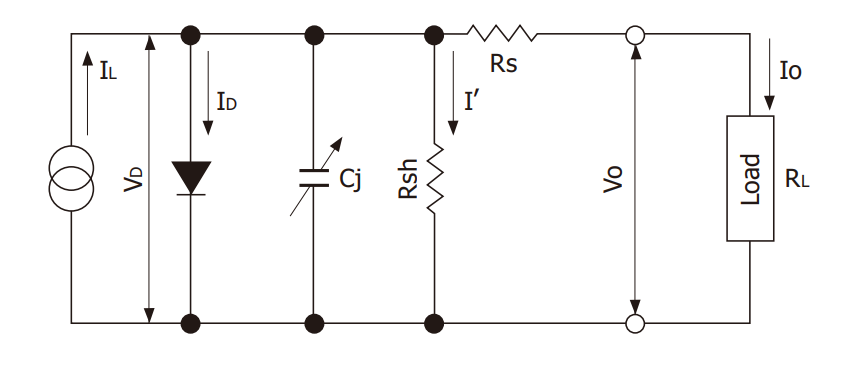
\includegraphics[width=0.7\textwidth]{figuras/3_circuitoequivalente.png}
  \caption{Circuito equivalente del fotodiodo con fuente de corriente. (Fuente: Hamamatsu \cite{hamamatsu2025}).}
  \label{fig:modelo_fotodiodo}
\end{figure}

\subsection{Respuesta temporal y detección del pico}
\label{subsec:respuesta_temporal}

Dado que en el sistema HSRL de Pilar el láser host emite pulsos de muy corta duración (entre 4~ns y 6~ns, propios del láser Surelite~II utilizado \cite{sureliteii}), la señal de cada disparo es un transitorio rápido cuyo tratamiento exige atender a la velocidad de respuesta del fotodiodo. Ésta se cuantifica mediante el tiempo de subida $t_r$ (intervalo en que la salida pasa del 10\% al 90\% de su valor de pico), determinado por tres factores: la constante de tiempo $t_1$ asociada a la capacidad de terminal $C_t$ y la resistencia de carga $R_L$, el tiempo de difusión $t_2$ de los portadores generados fuera de la zona de deplexión, y el tiempo de tránsito $t_3$ de los portadores dentro de ella \cite{hamamatsu2025}:

\begin{equation}
  t_1 = 2{,}2\,C_t\,R_L, \qquad
  t_3 \approx \frac{d^2}{\mu\,V_R}, \qquad
  t_r = \sqrt{t_1^{2} + t_2^{2} + t_3^{2}},
  \label{eq:tiempo_subida}
\end{equation}

\noindent con $d$ el ancho de la zona de deplexión, $\mu$ la movilidad de los portadores y $V_R$ la tensión inversa aplicada. El ancho de banda efectivo del detector se relaciona con el tiempo de subida mediante

\begin{equation}
  f_c = \frac{0{,}35}{t_r}.
  \label{eq:ancho_banda}
\end{equation}

Estas expresiones indican que, para seguir fielmente un pulso de pocos nanosegundos, el conjunto fotodiodo--TIA debe presentar un tiempo de subida menor que la duración del pulso, esto es, un ancho de banda del orden de decenas a cientos de MHz. Aun cumpliendo esa condición, dada la brevedad del pulso, la información relevante de cada disparo no es la forma completa de la señal sino su valor de pico, correspondiente al instante de máxima iluminación del fotodiodo. Cuando la fuente de luz se apaga ($I_L = 0$), la corriente de salida decae exponencialmente hacia la corriente oscura. Este comportamiento se observa en la Figura~\ref{fig:senal_pico}, que muestra la respuesta de los cuatro fotodiodos del circuito de sintonización al pulso de luz de corta duración.

\begin{figure}[h]
  \centering
  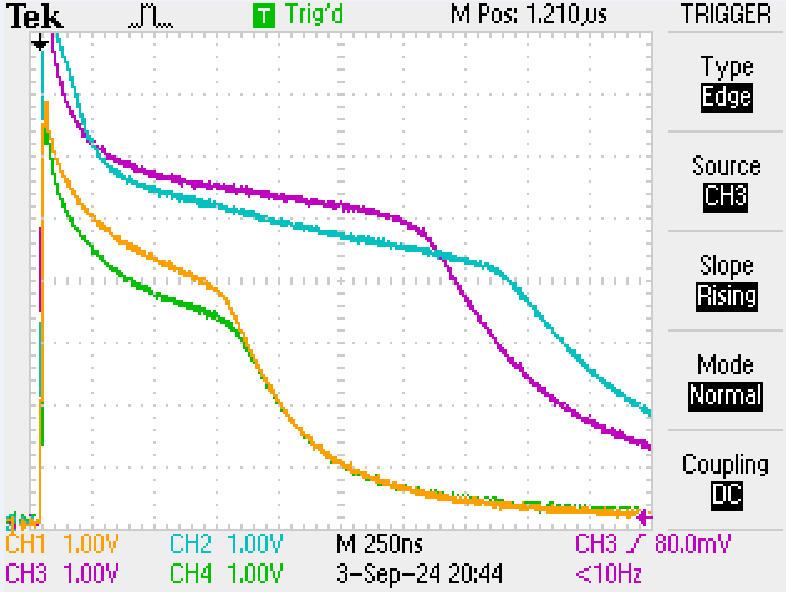
\includegraphics[width=0.7\textwidth]{figuras/3_señalesfotodiodos.png}
  \caption{Señal de salida de los cuatro fotodiodos del circuito de sintonización. (Fuente: elaboración propia).}
  \label{fig:senal_pico}
\end{figure}

Por lo tanto, la información relevante de la señal de salida de cada fotodiodo es su valor de pico, magnitud que debe ser detectada y digitalizada para permitir el control de sintonización.


\part{Marco Metodológico}
% =============================================================
% Capítulo 4 - Diseño del circuito de detección de picos
% =============================================================
\chapter{Diseño del circuito de detección de picos}
\label{cap:diseno_deteccion_picos}

Para determinar el valor máximo de la señal de salida del fotodiodo correspondiente al lazo de sintonización se plantearon dos alternativas tecnológicas:

\begin{itemize}
  \item Digitalizar la señal completa mediante un conversor analógico-digital (ADC) de alta velocidad y procesarla posteriormente por software para localizar el valor máximo.
  \item Retener el valor máximo de la señal analógica mediante un circuito detector de picos y digitalizar dicho valor con un ADC de menor velocidad.
\end{itemize}

Por razones de costo e implementación, se adoptó la segunda alternativa, ya que permite emplear un ADC de menor velocidad de muestreo y costo reducido, disminuyendo simultáneamente el volumen de datos a procesar por el microcontrolador.

\section{Modelado del circuito de detección}
\label{sec:modelado_simulacion}

El circuito detector de picos diseñado consta de dos amplificadores realimentados por corriente (CFA), conectados en configuración no inversora, y un transistor bipolar que opera como elemento detector y buffer de carga. 

En la Figura \ref{fig:detector} se ilustra el esquema eléctrico del detector propuesto para el canal $P_+$. El amplificador $\text{U1A}$ está configurado como no inversor con una ganancia $G = +2$, donde la resistencia $R_1$ adapta la impedancia proveniente del amplificador de transimpedancia del fotodetector. El transistor $Q_1$ se emplea como diodo detector mediante su unión base-emisor y se encarga de cargar el circuito $RC$ conformado por $R_3$ y $C_1$. El amplificador $\text{U1B}$ actúa como separador (\emph{buffer}) de salida con ganancia unitaria, evitando que la impedancia de entrada del ADC descargue el capacitor de retención antes de completar la conversión. El empleo de integrados CFA, en lugar de los amplificadores realimentados por tensión (VFA) convencionales, permite alcanzar un elevado \emph{slew rate}, condición determinante para seguir la rápida variación temporal de la señal proveniente del fotodiodo.

\begin{figure}[h]
  \centering
  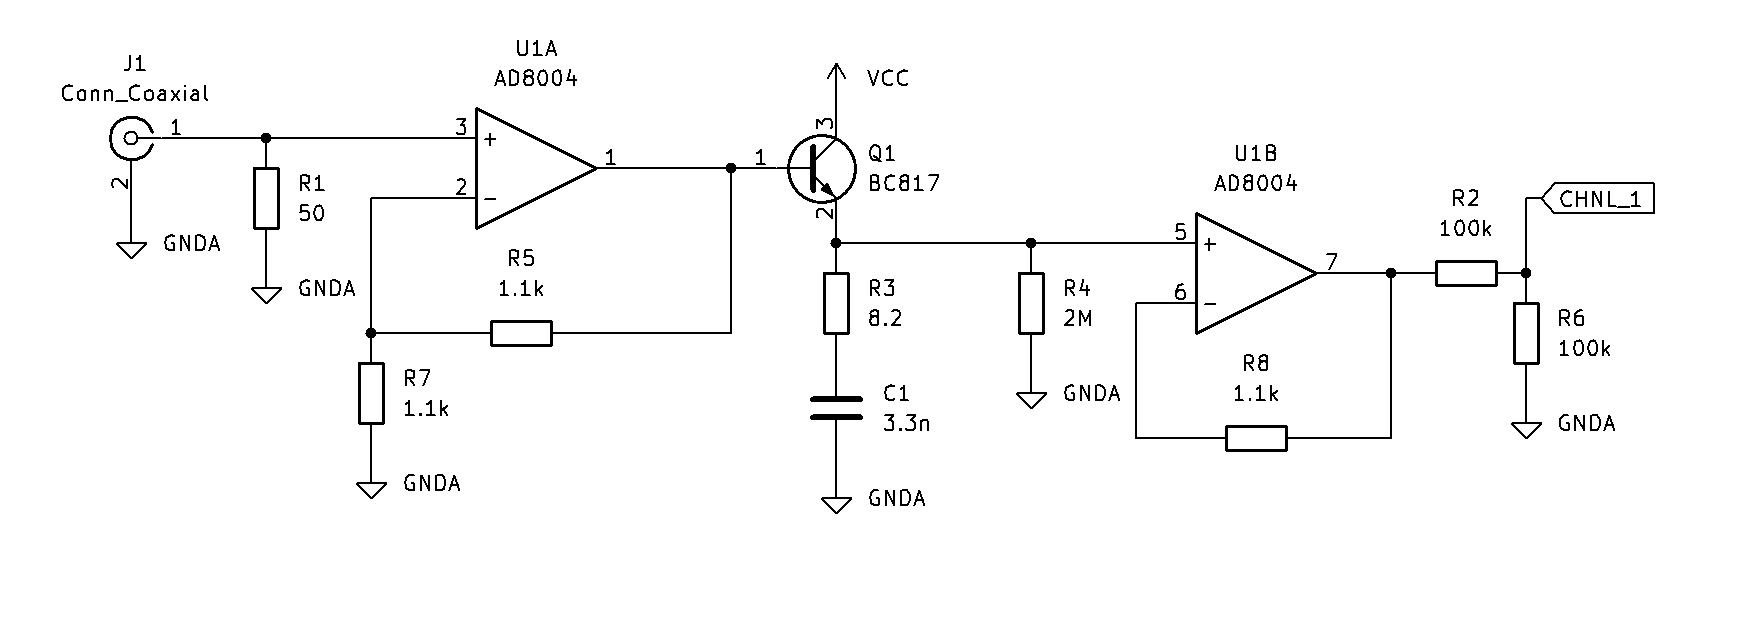
\includegraphics[width=0.8\textwidth]{figuras/4_detectordepicos.png}
  \caption{Circuito detector de picos para el canal $P_+$ (Fuente: elaboración propia).}
  \label{fig:detector}
\end{figure}

El amplificador $\text{U1A}$ se configuró con una ganancia de 2 para extender el rango dinámico del circuito. Ante niveles bajos de señal a la entrada del detector (derivados de una atenuación severa del haz láser), se presentan dos limitaciones principales: la no linealidad intrínseca de la unión base-emisor del transistor a bajas corrientes y la excursión máxima de salida (\emph{Output Voltage Swing}) del amplificador operacional. De esta forma, se logra un compromiso adecuado entre la linealidad del circuito para niveles altos de excitación y la sensibilidad a señales débiles.

Partiendo de la ecuación diferencial de carga de un circuito $RC$,

\begin{equation}
  V_C(t) = V_O \left(1 - e^{-\frac{t}{R_3 C_1}}\right)
  \label{eq:carga_rc}
\end{equation}

\noindent y considerando que para tiempos $t / (R_3 C_1) \ll 1$ la exponencial puede aproximarse mediante su serie de Taylor de primer orden como:

\begin{equation}
  V_C(t) \approx V_O \, \frac{t}{R_3 C_1},
  \label{eq:carga_rc_lineal}
\end{equation}

\noindent se obtiene una relación lineal entre la tensión retenida y la tensión de pico de entrada sin necesidad de cargar completamente el capacitor $C_1$. Esto permite seleccionar valores de capacidad que otorguen tiempos de descarga suficientemente prolongados para digitalizar el valor de pico $V_O$ empleando un conversor de velocidad moderada.

\section{Selección de componentes activos}

El amplificador realimentado por corriente AD8004 fue seleccionado debido a su elevado \emph{slew rate} (resumido en la Tabla \ref{tab:caracteristicas_ad8004}) y su bajo costo. La integración de cuatro amplificadores operacionales en un mismo encapsulado permite reducir la superficie de la placa y garantizaría, por lo menos en teoría, que ambos canales experimenten la misma deriva térmica.

\begin{table}[h]
  \centering
  \begin{tabular}{lll}
    \toprule
    \textbf{Parámetro} & \textbf{Valor} & \textbf{Condiciones} \\
    \midrule
    \multicolumn{3}{l}{\textit{Desempeño dinámico}} \\
    Ancho de banda ($-3$~dB)            & 250~MHz             & $G = +1$          \\
    Ancho de banda (planitud 0,1~dB)    & 30~MHz              & $G = +2$          \\
    Slew rate                           & 3000~V/\textmu s   & $V_S = \pm5$~V    \\
    Slew rate                           & 1100~V/\textmu s   & $V_S = +5$~V      \\
    Tiempo de establecimiento (0,1\,\%) & 21~ns               &                   \\
    Tiempo de subida (escalón de 2~V)   & 1,8~ns              &                   \\
    \midrule
    \multicolumn{3}{l}{\textit{Desempeño DC y características de entrada}} \\
    Tensión de \emph{offset} de entrada     & 1,0~mV (típ.); 3,5~mV (máx.) &                \\
    Corriente de polarización de entrada    & $\pm40$~\textmu A (típ.)      &                \\
    Transresistencia en lazo abierto        & 290~k$\Omega$                & $V_O = \pm2.5$~V \\
    Resistencia de entrada (no inversora)   & 2~M$\Omega$                  &                \\
    Rango de tensión de entrada (modo común)& 3,2~V                        &                \\
    \midrule
    \multicolumn{3}{l}{\textit{Salida y alimentación}} \\
    Corriente de salida                     & 50~mA               &                        \\
    Corriente de alimentación por amplif.   & 3,5~mA (35~mW)      &                        \\
    Rango de alimentación (simple)          & +4 a +12~V          &                        \\
    Rango de alimentación (dual)            & $\pm2$ a $\pm6$~V   &                        \\
    Tensión de alimentación máxima          & 12,6~V              & Valor máximo absoluto  \\
    Rango de temperatura de operación       & $-40$ a $+85$~$^{\circ}$C & Grado A          \\
    Encapsulado                             & SOIC de 14 pines    &                        \\
    \bottomrule
  \end{tabular}
  \caption{Características principales del amplificador realimentado por corriente AD8004 (Fuente: adaptado de \cite{ad8004_ds}).}
  \label{tab:caracteristicas_ad8004}
\end{table}

Como elemento detector se empleó un transistor bipolar NPN BC817, cuya alta capacidad de corriente de colector ($I_C = 500\,\text{mA}$, véase la Tabla \ref{tab:caracteristicas_bc817}) resulta indispensable para cargar rápidamente el capacitor acoplado a su emisor.

\begin{table}[h]
  \centering
  \begin{tabular}{lll}
    \toprule
    \textbf{Parámetro} & \textbf{Valor} & \textbf{Condiciones} \\
    \midrule
    \multicolumn{3}{l}{\textit{Valores máximos absolutos}} \\
    Tensión colector-base ($V_{CBO}$)   & 50~V             & $I_E = 0$        \\
    Tensión colector-emisor ($V_{CEO}$) & 45~V             & $I_B = 0$        \\
    Tensión emisor-base ($V_{EBO}$)     & 5~V              & $I_C = 0$        \\
    Corriente de colector ($I_C$)       & 500~mA           & Continua         \\
    Potencia de disipación ($P_D$)      & 300~mW           & $T_A = 25$~$^{\circ}$C \\
    Temperatura de unión ($T_J$)        & 150~$^{\circ}$C  & Máxima           \\
    \midrule
    \multicolumn{3}{l}{\textit{Características eléctricas}} \\
    Ganancia de corriente DC ($h_{FE}$)      & 160 a 400            & $V_{CE}=1$~V, $I_C=100$~mA \\
    Tensión de saturación C-E ($V_{CE(\text{sat})}$)& 0,7~V (máx.)         & $I_C=500$~mA, $I_B=50$~mA  \\
    Tensión de saturación B-E ($V_{BE(\text{sat})}$)& 1,2~V (máx.)         & $I_C=500$~mA, $I_B=50$~mA  \\
    Frecuencia de transición ($f_T$)         & 100~MHz (mín.)       & $V_{CE}=5$~V, $I_C=10$~mA  \\
    \midrule
    \multicolumn{3}{l}{\textit{Datos generales}} \\
    Tipo        & NPN de silicio, propósito general & \\
    Encapsulado & SOT-23                            & \\
    \bottomrule
  \end{tabular}
  \caption{Características principales del transistor bipolar NPN BC817 (Fuente: adaptado de \cite{bc817_ds}).}
  \label{tab:caracteristicas_bc817}
\end{table}

\section{Selección de componentes pasivos}

Para el dimensionamiento de los componentes pasivos del circuito se consideraron los siguientes criterios de diseño:
\begin{itemize}
  \item La resistencia de polarización de emisor $R_4$ debe ser suficientemente alta para no descargar el capacitor $C_1$ antes de la conversión analógico-digital, pero adecuada para establecer un punto de operación estable en reposo.
  \item La constante de tiempo $\tau = R_3 C_1$ debe garantizar la aproximación lineal descrita en la Ecuación \ref{eq:carga_rc_lineal} durante el pulso de entrada. Este criterio es el que fija el valor de $R_3$.
  \item La corriente de pico que impone $R_3$ sobre el transistor $Q_1$ debe resultar admisible para el régimen impulsivo de trabajo, lo que se verifica en términos de energía por pulso y potencia media disipada.
  \item Las redes de realimentación para $\text{U1A}$ y $\text{U1B}$ se ajustaron según las recomendaciones del fabricante del AD8004 para optimizar la respuesta en frecuencia y asegurar la estabilidad en lazo cerrado.
\end{itemize}

\subsection{Cálculo de la constante de tiempo del circuito RC}

A partir de las caracterizaciones experimentales de la señal entregada por los fotodetectores se determinó que el pulso útil tiene una duración aproximada de $2\,\text{ns}$, seguido de un decaimiento exponencial que ya no contribuye a la carga del capacitor de retención. Para que dicha carga permanezca en la zona lineal descrita por la Ecuación \ref{eq:carga_rc_lineal} debe cumplirse $t \ll \tau = R_3 C_1$, condición que fija un valor objetivo de constante de tiempo del orden de las decenas de nanosegundos.

Adoptando un valor comercial E24 estándar de $R_3 = 8{,}2\,\Omega$ junto con un capacitor $C_1 = 3{,}3\,\text{nF}$, se obtiene una constante de tiempo efectiva de:

\begin{equation}
  \tau = R_3 C_1 = 8{,}2\,\Omega \times 3{,}3\,\text{nF} = 27{,}06\,\text{ns}
  \label{eq:tau_final}
\end{equation}

Fijado $R_3$ por el criterio anterior, queda verificar que la corriente que atraviesa el transistor $Q_1$ sea admisible. El valor adoptado impone una corriente de pico inicial:

\begin{equation}
  I_0 = \frac{V_{O,\text{U1A}} - V_{BE}}{R_3} = \frac{12\,\text{V} - 1{,}2\,\text{V}}{8{,}2\,\Omega} = 1{,}32\,\text{A}
  \label{eq:valor_r3_calc}
\end{equation}

\noindent valor superior a la corriente máxima de pico $I_{CM} = 1\,\text{A}$ que declara la hoja de datos del BC817 \cite{bc817_ds}. Dicho límite, sin embargo, está especificado para pulsos de $20\,\text{ms}$, un régimen en el que el calor generado alcanza a difundir hacia el encapsulado y la restricción es de naturaleza térmica. En la aplicación presente el pulso dura $2\,\text{ns}$, seis órdenes de magnitud menos, por lo que corresponde verificar la disipación efectiva en lugar de aplicar el límite de forma directa.

Con una caída colector-emisor $V_{CE} \approx 1{,}2\,\text{V}$ y una corriente media de $1{,}27\,\text{A}$ durante el pulso, la potencia instantánea alcanza $1{,}58\,\text{W}$ y la energía depositada en la juntura por cada disparo resulta:

\begin{equation}
  E_{pulso} = V_{CE}\, \bar{I}_C\, t = 1{,}2\,\text{V} \times 1{,}27\,\text{A} \times 2\,\text{ns} = 3{,}05\,\text{nJ}
  \label{eq:energia_pulso_q1}
\end{equation}

A la frecuencia de repetición del láser de $20\,\text{Hz}$, el ciclo de trabajo es de $4\times10^{-8}$ y la potencia media disipada por $Q_1$ asciende a $61\,\text{nW}$, seis órdenes de magnitud por debajo de los $250\,\text{mW}$.

 El transistor opera por lo tanto muy lejos de su límite térmico, y el valor de $I_{CM}$ de la hoja de datos debe interpretarse como una cota de régimen continuo y no como una restricción activa del diseño.


\subsection{Cálculo de la red de polarización del transistor}

El transistor $Q_1$ opera en configuración seguidor de emisor (colector común), actuando como buffer de tensión que permite al amplificador $\text{U1A}$ cargar el nodo capacitivo con valores pico superiores a la capacidad de salida del propio OPAMP.

Dado que la etapa no cuenta con excursión \emph{rail-to-rail}, en ausencia de señal de entrada la tensión de salida continua en reposo del $\text{U1A}$ es de aproximadamente $1\,\text{V}$. Para evitar la descarga prematura del capacitor de retención a través de $R_4$, se impuso la condición $R_4 \gg R_3$, seleccionándose $R_4 = 82\,\text{k}\Omega$.

La corriente de reposo de emisor resulta:

\begin{equation}
  I_E = \frac{V_{O,\text{U1A}} - V_{BE}}{R_4} = \frac{1\,\text{V} - 0{,}58\,\text{V}}{82\,\text{k}\Omega} = 5{,}12\,\mu\text{A}
  \label{eq:transistor_ie}
\end{equation}

Cabe señalar que la tensión base-emisor empleada en la Ecuación \ref{eq:transistor_ie} difiere de la utilizada en la Ecuación \ref{eq:valor_r3_calc}. Ello responde a que $V_{BE}$ depende de la corriente de colector: el valor de $1{,}2\,\text{V}$ corresponde al régimen impulsivo de amperes durante el pico, mientras que los $0{,}58\,\text{V}$ corresponden al régimen de reposo, de algunos microamperes.

Esta pequeña corriente de polarización mantiene al transistor en el límite de la zona activa sin comprometer la retención de carga en $C_1$. En la Tabla \ref{tab:componentes_pasivos} se resumen los valores y características de los componentes pasivos adoptados.

\begin{table}[h]
  \centering
  \begin{tabular}{c c c c l}
    \toprule
    \textbf{Componente} & \textbf{Valor} & \textbf{Tolerancia} & \textbf{Encapsulado} & \textbf{Función técnica} \\
    \midrule
    $R_1$ & $50\,\Omega$ & $\pm 1\%$ & SMD 0603 & Adaptación de impedancia de entrada \\
    $R_2$ & $1\,\text{k}\Omega$ & $\pm 1\%$ & SMD 0603 & Red de realimentación U1A ($G=+2$) \\
    $R_3$ & $8{,}2\,\Omega$ & $\pm 1\%$ & SMD 0603 & Limitador de corriente de carga del capacitor \\
    $R_4$ & $82\,\text{k}\Omega$ & $\pm 1\%$ & SMD 0603 & Polarización de reposo de emisor ($Q_1$) \\
    $R_f$ & $1\,\text{k}\Omega$ & $\pm 1\%$ & SMD 0603 & Resistencia de lazo CFA (estabilidad U1A/U1B) \\
    $C_1$ & $3{,}3\,\text{nF}$ & $\pm 5\%$ & SMD 0603 (NP0/C0G) & Capacitor de retención de tensión de pico \\
    \bottomrule
  \end{tabular}
  \caption{Componentes pasivos seleccionados para el circuito detector de picos (Fuente: elaboración propia).}
  \label{tab:componentes_pasivos}
\end{table}

\section{Simulación del circuito detector de picos}
\label{sec:simulacion_circuito_detector}

La simulación del circuito se ejecutó tomando como señal de excitación una captura osciloscópica real de la salida del fotodiodo (Figura \ref{fig:pulso}). Como entorno de simulación se utilizó el motor NGSPICE v46 integrado con la interfaz gráfica QUCS-S (Figura \ref{fig:sim}).

\begin{figure}[htbp]
  \centering
  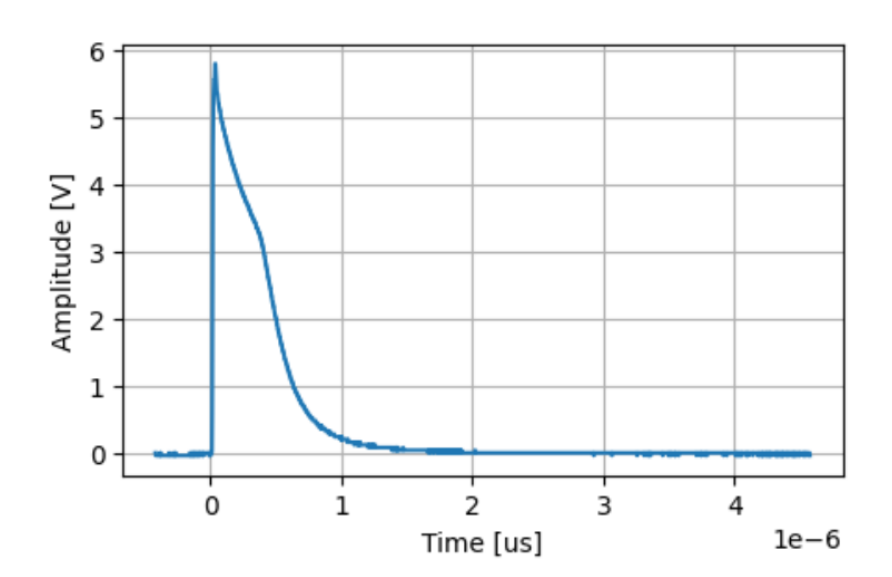
\includegraphics[width=0.6\textwidth]{figuras/4_señalpulso.png}
  \caption{Señal pulsada $P_+$ capturada mediante osciloscopio Tektronix (Fuente: elaboración propia).}
  \label{fig:pulso}
\end{figure}

\begin{figure}[htbp]
  \centering
  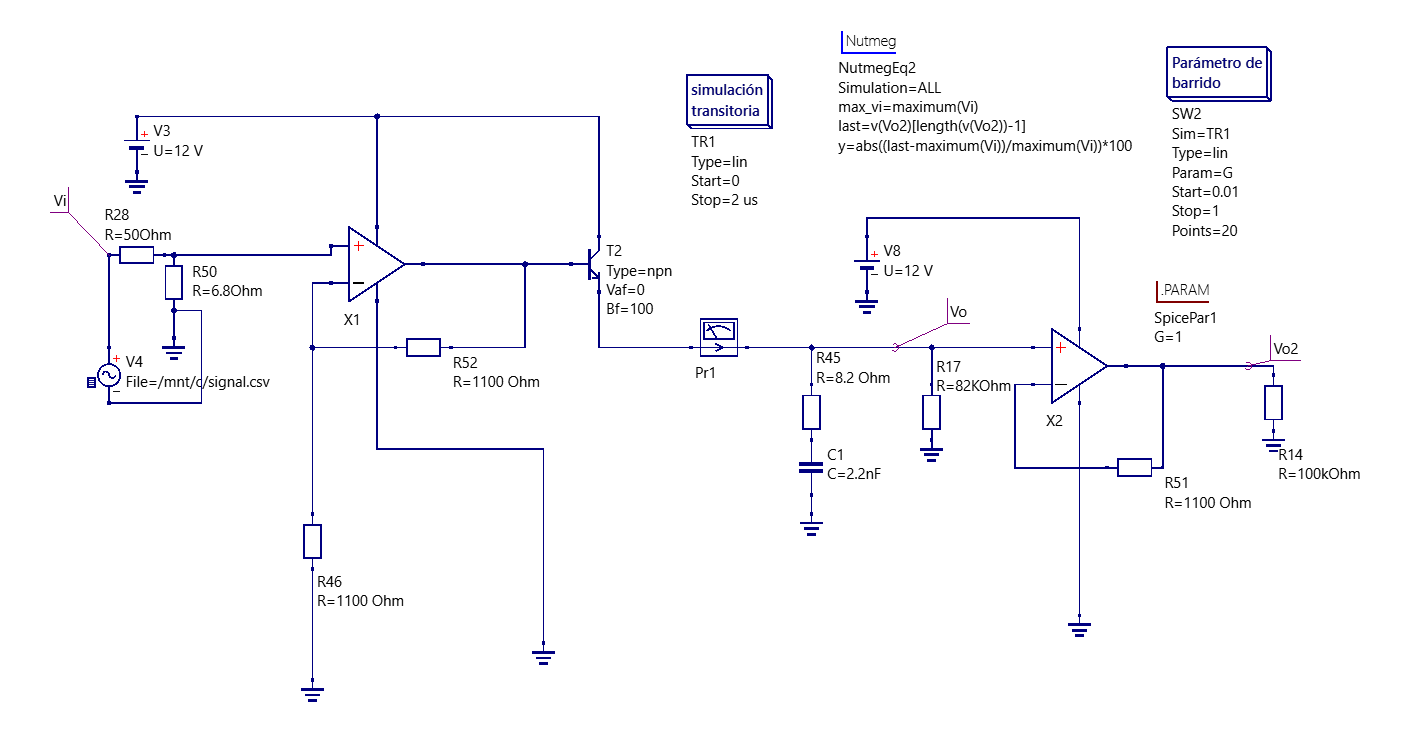
\includegraphics[width=1\textwidth]{figuras/4_simulacion.png}
  \caption{Esquema del circuito detector implementado en QUCS-S (Fuente: elaboración propia).}
  \label{fig:sim}
\end{figure}

Se ejecutó un análisis de barrido paramétrico (\emph{DC/Transient sweep}) de 25 valores de tensión de entrada $V_{\text{in}}$ (Figura \ref{fig:barrido}). Los resultados confirman una respuesta lineal para tensiones de entrada $V_{\text{in}} \ge 0{,}8\,\text{V}$ (Figura \ref{fig:linealidad}), límite impuesto por el piso de tensión del amplificador operando bajo fuente simple de $+12\,\text{V}$.

\begin{figure}[htbp]
  \centering
  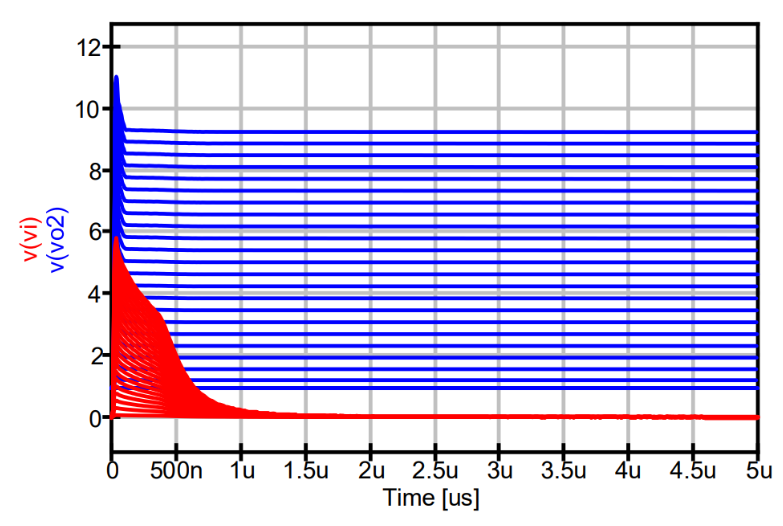
\includegraphics[width=0.7\textwidth]{figuras/4_simbarrido.png}
  \caption{Barridos temporales de la tensión de salida para distintos niveles de $V_{\text{in}}$ (Fuente: elaboración propia).}
  \label{fig:barrido}
\end{figure}

La tensión retenida por el detector fue evaluada a los $5\,\mu\text{s}$ posteriores al pico de entrada. Este intervalo responde al tiempo necesario para que un ADC comercial de costo moderado (con tasa de muestreo de $500\,\text{ksps}$) realice el ciclo de muestreo y retención (\emph{Sample \& Hold}) sin introducir errores temporales.

\begin{figure}[htbp]
  \centering
  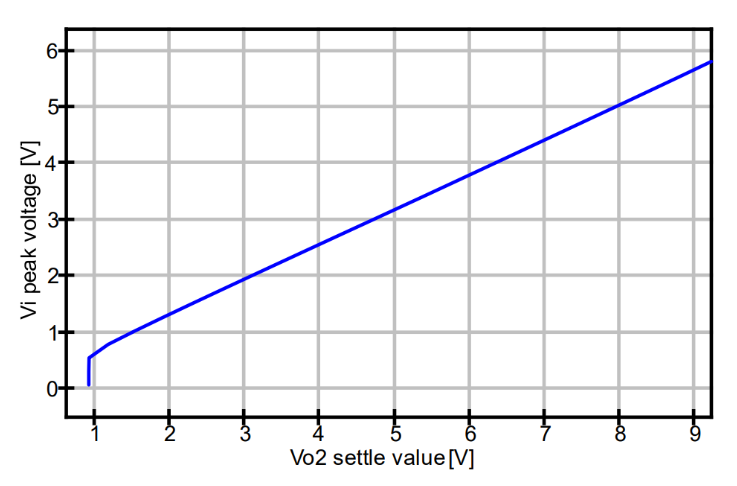
\includegraphics[width=0.7\textwidth]{figuras/4_simlinealidad.png}
  \caption{Tensión de salida $V_O$ medida a $t = 5\,\mu\text{s}$ en función de la tensión de pico de entrada $V_{\text{in}}$ (Fuente: elaboración propia).}
  \label{fig:linealidad}
\end{figure}

Este rango de operación se considera correcto como se verá en el Capítulo \ref{cap:modelo_experimental}, puesto que los valores de tensión que realmente importan para controlar el HSRL son definidos a criterio del operador, en torno a los mínimos de $P_+$ y $P_-$. Además, poseemos dos grados de libertad para mantenernos en la zona lineal del detector, relacionados con la intensidad de los haces de referencia:

\begin{itemize}
  \item Densidad óptica del filtro neutro, mostrado en la figura \ref{fig:diagrama_hsrl}.
  \item Absorción óptica de la celda de iodo de referencia, explicado en el Capítulo \ref{cap:lidar_hsrl}.
\end{itemize}

\section{Prototipado y validación experimental}
\label{sec:prototipado_validacion}

Se fabricó un primer prototipo en laboratorio mediante la técnica de transferencia térmica y grabado químico con cloruro férrico. Se montaron componentes de tecnología de montaje superficial (SMD) para minimizar el impacto de las componentes parásitas.

Al someter el circuito a un pulso de prueba de $100\,\text{ns}$ de ancho a una frecuencia de repetición de $20\,\text{Hz}$, la respuesta temporal presentó oscilaciones severas en el nodo de salida (véase la Figura \ref{fig:oscilaciones}). Este comportamiento inestable fue provocado por capacidades parásitas acopladas a los nodos de alta impedancia de los amplificadores CFA, degradando fuertemente la linealidad del detector.

\begin{figure}[htbp]
  \centering
  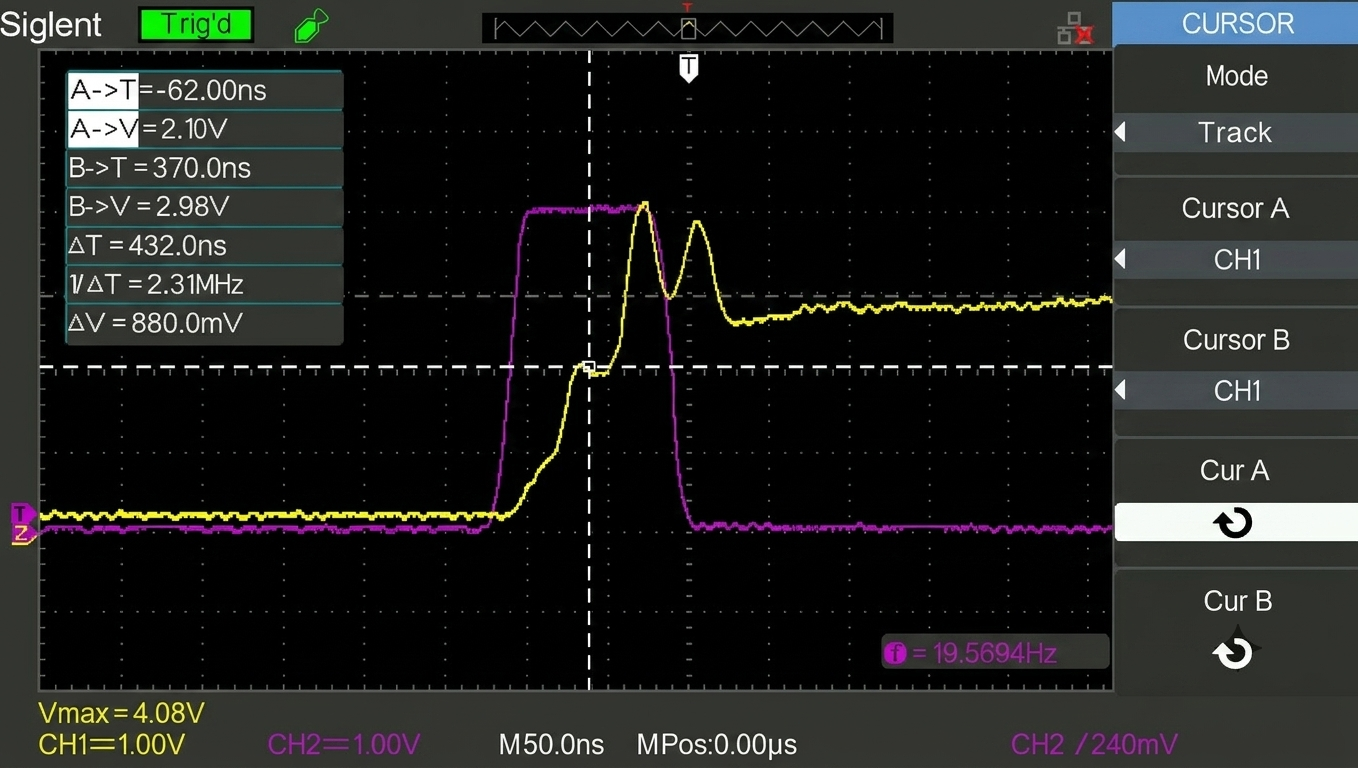
\includegraphics[width=0.8\textwidth]{figuras/4_oscilacion.png}
  \caption{Respuesta del prototipo ante un pulso de $100\,\text{ns}$ ($20\,\text{Hz}$), evidenciando oscilaciones de alta frecuencia derivadas de parásitos del trazado (Fuente: elaboración propia; imagen procesada con inteligencia artificial \cite{nanobananapro}).}
  \label{fig:oscilaciones}
\end{figure}

Ante esta problemática, previo a continuar con los ensayos en laboratorio, se decidió diseñar un nuevo circuito impreso (PCB) multicapa optimizado para aplicaciones de alta frecuencia. En esta fase integradora se incorporaron también el microcontrolador de control del sistema (desarrollado en la Sección \ref{sec:rp2350}) y los transceptores para la interfaz de comunicación serie con el sistema \emph{seeder} (Sección \ref{sec:rs232_uart}).

El análisis detallado sobre el diseño de la placa final y validación del circuito analógico se desarrolla en mayor detalle en el Capítulo \ref{cap:placacontrol}.


% =============================================================
% Capitulo 5 - Seleccion del microcontrolador y arquitectura general
% =============================================================

\chapter{Selección del microcontrolador y arquitectura general de periféricos}
\label{cap:micro}
\section{Requisitos de diseño}

Como base para el software de control, se partió del programa previamente desarrollado por el NIES, descrito en el Anexo \ref{anexo:hsrlnies}. Este software, pese a tener problemas de estabilidad y de compatibilidad con los sistemas operativos actuales, sirvió como referencia para definir la potencia de cómputo necesaria que debería tener el microcontrolador a seleccionar. 

Además, se tomaron los siguientes requisitos de periféricos para el microcontrolador a usar:

\begin{itemize}
    \item \textbf{Comunicación con PC:} realizada mediante un puerto USB.
    \item \textbf{Comunicación con seeder:} mediante puerto serie, usando RS-232.
    \item \textbf{Digitalización de señal del detector de picos:} utilizando un ADC. Idealmente el mismo del microcontrolador para reducir cantidad de componentes y costo.
    \item \textbf{Detección de flanco de sincronía del láser}: con GPIO de uso general.
\end{itemize}

\section{Microcontroladores de la familia RP2350}
\label{sec:rp2350}

Se seleccionó un RP2350 (presente en la placa de desarrollo Raspberry Pi Pico~2) como microcontrolador del sistema debido a su bajo costo y a su documentación técnica completa y accesible. Además, al contar con dos interfaces UART, USB nativo y 26 pines GPIO, no sólo permite la comunicación con el \emph{seeder} y la PC, sino que además habilita la expansión del sistema en caso de ser necesario. Para el prototipo de la placa de control se utilizó el módulo comercial Raspberry Pi Pico 2 como referencia de diseño.

Sus dos núcleos permiten correr en paralelo lecturas y escrituras de puerto serie y la digitalización de la señal, sin necesidad de utilizar sistemas de división de tareas o interrupciones específicas mediante timers. Las características más importantes del microcontrolador se resumen en la Tabla \ref{tab:rp2350} \cite{rp2350_datasheet}. El agregado de protocolo I2C también permite ampliar al sistema con un diverso rango de sensores compatibles con este protocolo. El diagrama de pinouts del mismo se representa en la Figura \ref{fig:pinout}.

\begin{figure}
    \centering
    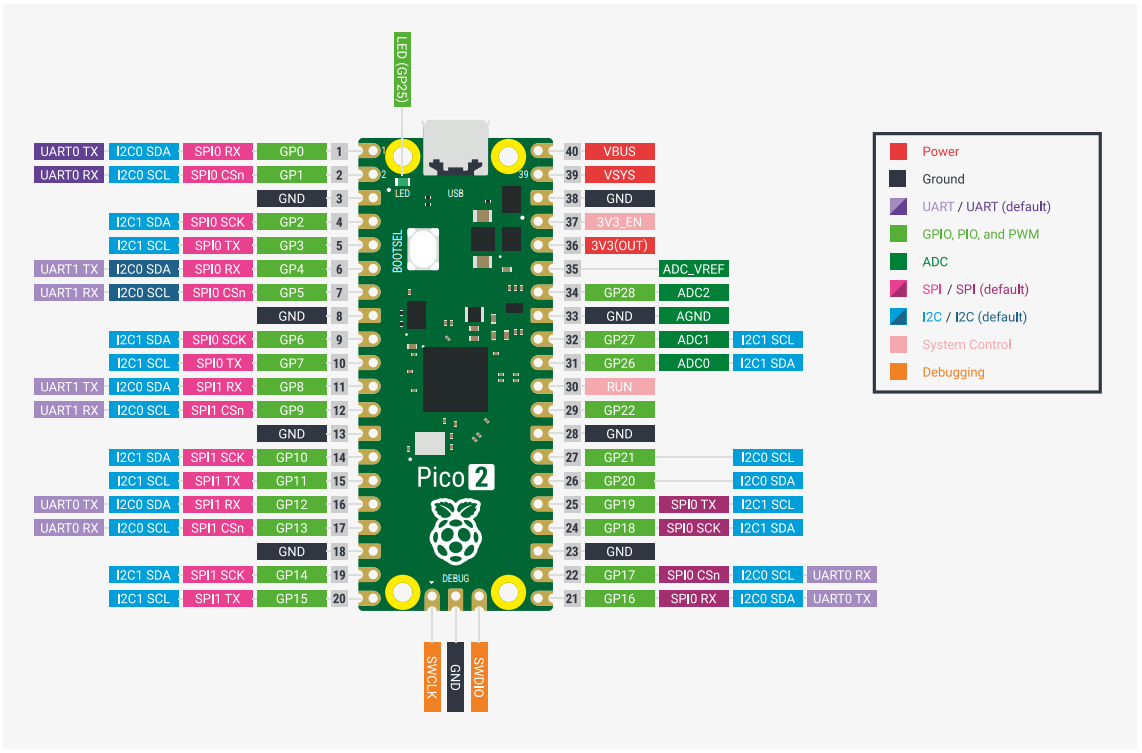
\includegraphics[width=0.8\textwidth]{figuras/5_pinout.png}
    \caption{Pinout de la placa de desarrollo Raspberry Pi Pico 2 (Fuente: adaptado de \cite{rp2350_datasheet}).}
    \label{fig:pinout}
\end{figure}

\begin{table}[h]
\centering
\renewcommand{\arraystretch}{1.3}
\begin{tabularx}{0.9\textwidth}{>{\bfseries}l X}
\toprule
Característica & \textbf{Especificación (Microcontrolador RP2350)} \\
\midrule
Arquitectura & Doble núcleo ARM Cortex-M33 / Doble núcleo Hazard3 RISC-V \\
Frecuencia de reloj & 150 MHz \\
Memoria SRAM & 520 KB integrada \\
Pines GPIO (RP2350A) & 30 en total (26 expuestos en la placa Pico 2) \\
Periféricos estándar & 2 $\times$ UART, 2 $\times$ SPI, 2 $\times$ I2C \\
Canales PWM & 24 canales \\
Convertidor A/D (ADC) & 4 canales de 12 bits \\
E/S Programable (PIO) & 3 bloques PIO (12 máquinas de estado en total) \\
Seguridad & ARM TrustZone, Secure Boot, SRAM con Anti-tamper, 8 KB OTP \\
\bottomrule
\end{tabularx}
\vspace{0.2cm}
\caption{Especificaciones destacadas del RP2350, utilizado en la Raspberry Pi Pico 2 (Fuente: adaptado de \cite{rp2350_datasheet}).}
\label{tab:rp2350}
\end{table}

Durante la selección del microcontrolador se evaluaron otras alternativas disponibles comercialmente, tales como el STM32F103C8T6 o el ESP32-WROOM-32. Como se resume en la Tabla \ref{tab:comparacion_micro}, ninguna de las tres opciones presenta limitaciones de cómputo frente a los requisitos planteados, por lo que la decisión se apoyó en
criterios de periféricos, documentación, costo, disponibilidad y familiaridad previa.
El ESP32-WROOM-32 fue descartado por carecer de interfaz USB nativa (obligando a incorporar un puente USB-serie adicional en la placa). El STM32F103C8T6, si bien es la opción de menor costo y con mejor ADC, posee documentación más diluida lo que podría aumentar los tiempos de desarrollo.

\begin{table}[h]
\centering
\renewcommand{\arraystretch}{1.3}
\begin{tabularx}{\textwidth}{>{\bfseries}l X X X}
\toprule
Criterio & \textbf{RP2350 (Pico 2)} & \textbf{STM32F103C8T6} & \textbf{ESP32-WROOM-32} \\
\midrule
Núcleos / frecuencia & 2 $\times$ Cortex-M33 @ 150 MHz & 1 $\times$ Cortex-M3 @ 72 MHz & 2 $\times$ Xtensa LX6 @ 240 MHz \\
SRAM & 520 KB & 20 KB & 520 KB \\
Memoria de programa & 4 MB QSPI externa & 64 KB Flash & 4 MB QSPI externa \\
ADC integrado & SAR 12 bits, 4 canales, 500 kS/s & SAR 12 bits, 10 canales, 1 MS/s & SAR 12 bits, 18 canales, con no linealidad y ruido documentados \\
UART & 2 & 3 & 3 \\
USB nativo & USB 1.1 device/host & USB 2.0 FS (solo device) & No posee; requiere puente USB-serie externo \\
GPIO expuestos & 26 & 32 & 34 (varios de solo entrada) \\
Documentación & Datasheet unificado y SDK en C con ejemplos oficiales & Reference manual extenso, aprendizaje pronunciado & Documentación repartida entre ESP-IDF y datasheet \\
Costo aproximado (placa) & USD 5--7 & USD 3--5 & USD 5--7 \\
Disponibilidad en distribuidores locales & Alta & Alta, aunque predominan clones no oficiales & Alta \\
Familiaridad previa & Sí & No & Parcial \\
\bottomrule
\end{tabularx}
\vspace{0.2cm}
\caption{Comparación de las alternativas de microcontrolador evaluadas (Fuente: elaboración propia a partir de \cite{rp2350_datasheet, stm32f103_datasheet, esp32_datasheet}).}
\label{tab:comparacion_micro}
\end{table}

\section{Selección del conversor analógico digital}

El microcontrolador RP2350 cuenta con un conversor analógico de cuatro canales de muestreo. Si bien durante el desarrollo del presente trabajo se trabajó únicamente con los canales $P_+$ y $P_-$, la lectura de los dos haces centrales $P_0$ puede constituir un dato de interés para el control del sistema. La disponibilidad de canales analógicos adicionales deja abierta esa posibilidad sin necesidad de modificar el hardware.

El microcontrolador RP2350 incorpora un convertidor analógico-digital de aproximaciones sucesivas (SAR) de 12 bits, cuya frecuencia de reloj de conversión \texttt{clk\_adc} opera nominalmente a $48\,\mathrm{MHz}$. Cada conversión completa (incluyendo la etapa de muestreo y retención y la posterior aproximación sucesiva) demanda 96 ciclos de dicho reloj, de donde se obtiene el tiempo de conversión mínimo:

\begin{equation}
    t_{\mathrm{conv}} = \frac{96\ \mathrm{ciclos}}{48 \times 10^{6}\,\mathrm{Hz}} = 2\,\mu\mathrm{s}
    \label{eq:tconv_rp2350}
\end{equation}

Este valor establece una frecuencia máxima de muestreo de $500\,\mathrm{kS/s}$. Tiempo suficiente para realizar el muestreo de la señal obtenida del detector de picos. La configuración del ADC en software, para máxima velocidad de conversión se encuentra detallada en la Tabla \ref{tab:config_adc}.


\begin{table}[h]
\centering
\begin{tabular}{lll}
\hline
\textbf{Parámetro} & \textbf{Valor} & \textbf{Constante} \\
\hline
Resolución & 12 bits & --- \\
Reloj del ADC & $48\,\mathrm{MHz}$ & --- \\
Divisor de reloj & 0 (máxima velocidad) & \texttt{ADC\_CLOCK\_DIV} \\
Ciclos por conversión & 96 & --- \\
Tiempo de conversión & $2\,\mu\mathrm{s}$ & --- \\
Frecuencia de muestreo total & $500\,\mathrm{kS/s}$ & --- \\
Canales activos & 2 (round-robin) & \texttt{ADC\_CHAN\_0/1} \\
Entradas analógicas & GPIO26, GPIO27 & \texttt{ADC\_GPIO\_0/1} \\
Frecuencia por canal & $250\,\mathrm{kS/s}$ & --- \\
Muestras por captura & 1024 (512 por canal) & \texttt{NUM\_SAMPLES} \\
Duración de la captura & $2{,}048\,\mathrm{ms}$ & --- \\
Disparo & Flanco ascendente, GPIO2 & \texttt{TRIGGER\_PIN} \\
Transferencia & DMA sincronizado por \texttt{DREQ\_ADC} & --- \\
\hline
\end{tabular}
\caption{Configuración del ADC del RP2350 en el sistema de adquisición (Fuente: elaboración propia).}
\label{tab:config_adc}
\end{table}


\section{Comunicación serie RS-232/UART}
\label{sec:rs232_uart}

La comunicación entre la placa de control y el láser \emph{seeder} se realiza mediante puerto serie estándar RS-232 especificado por el fabricante del equipo \cite{npphotonics_flm005}. Dado que los niveles de tensión RS-232
no son compatibles con los niveles de tensión lógicos del microcontrolador, es necesario un circuito integrado transceptor que adapte ambos.

\begin{figure}[htpb]
    \centering
    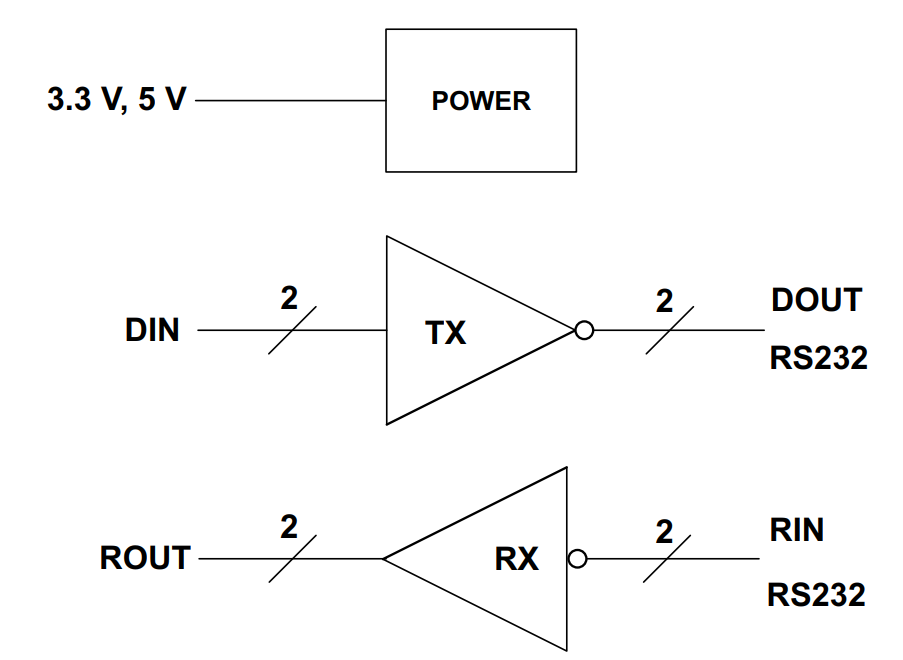
\includegraphics[width=0.6\textwidth]{figuras/5_max3232.png}
    \caption{Esquemático simplificado del transceptor MAX3232 (Fuente: adaptado de \cite{ti_max3232}).}
    \label{fig:max3232}
\end{figure}

Para la tarea de adaptar niveles de tensión se seleccionó el circuito integrado MAX3232 por su simplicidad de implementación, alta disponibilidad y baja cantidad de componentes requeridos. Además, gracias a la posibilidad de alimentarlo con 3,3~V \cite{ti_max3232}, es posible utilizar la salida del regulador de la misma placa de desarrollo Raspberry Pi Pico 2. Su diagrama simplificado se representa en la Figura \ref{fig:max3232}.


\section{Detección de la señal de sincronismo}

El láser \emph{host} provee una señal de sincronismo SYNC para detectar cuándo ocurre el disparo del mismo. Para la correcta digitalización, es necesario comenzar la conversión en el momento que el láser dispara para digitalizar el valor del detector de picos antes de que el mismo se descargue por completo.

Esta señal se adaptó de niveles TTL a niveles CMOS mediante el uso de un simple divisor resistivo, ilustrado en la Figura \ref{fig:divisor}.

Para la selección de resistencias

\begin{equation}
  3{,}3\,\text{V} = 5\,\text{V} \, \frac{R_{18}}{R_{17} + R_{18}}   
  \label{eq:div1}
\end{equation}

\noindent con $R_{17} = 1{,}8\,\text{k}\Omega$, se tiene

\begin{equation}
  R_{18} = \frac{1188}{0{,}34} \approx 3494{,}12\,\Omega \approx 3{,}494\,\text{k}\Omega  
  \label{eq:div2}
\end{equation}

\noindent por lo tanto según valores estándar E24 $R_{18} = 3{,}6\,\text{k}\Omega$

\begin{figure}[h]
    \centering
    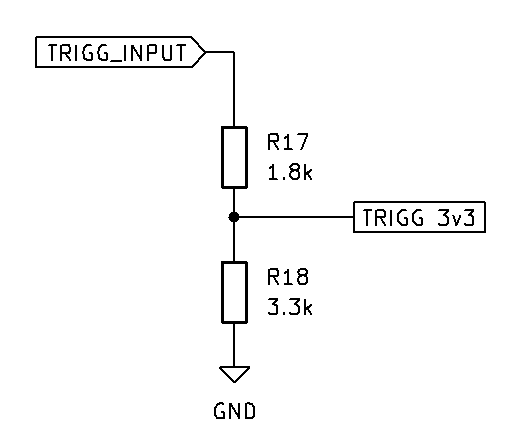
\includegraphics[width=0.5\textwidth]{figuras/5_divisor.png}
    \caption{Divisor resistivo para la señal de sincronismo del láser host (Fuente: elaboración propia).}
    \label{fig:divisor}
\end{figure}
\chapter{Diseño y validación de PCB}
\label{cap:placacontrol}

El diseño del PCB fue necesario para llegar terminar de validar el detección de picos y comunicación con el seeder, puesto que la mayoría de los componentes utilizados son circuitos integrados de montaje superficial. Para el diseño del mismo, siguiendo la línea del presente PI de utilizar software libre, KiCad V9.0.

\section{Circuito esquemático}
\label{sec:esquematico}

El circuito esquemático final integra los circuitos discutidos en el Capítulo \ref{cap:diseno_deteccion_picos} y \ref{cap:micro}. El esquemático desarrollado se divide en dos partes, el circuito analógico de detección y el circuito digital de comunicación y detección de trigger. Se omitió incluir en la placa elementos como reguladores de tensión, indicadores LED o pulsadores, debido a que para un primer prototipo se buscaba la simplificación y la validación de la sección analógica y de comunciación con el seeder. Una versión completa del circuito esquemático se encuentra en el Anexo \ref{anexo:esquematico}.

\section{Criterios de Diseño del PCB}

La placa se desarrolló tomando en cuenta buenas prácticas de ruteo y diseño electrónico, tales como


\begin{itemize}
  \item Mantenimiento de planos de masa con recortes (\emph{cutouts}) debajo de los pines de entrada y de la red de realimentación.
  \item Ubicación de los componentes de la red de realimentación lo más cerca posible del amplificador, las resistencias de realimentación $R_f$ conectadas directamente entre el pin de salida y el pin $-IN$ sin vías intermedias.
  \item Colocación de capacitores de desacople en los pines de alimentación, con vía directa al plano de masa. Particularmente capacitores de tantalio, según hoja de datos \cite{ad8004_ds}
  \item Separación de las pistas de entrada respecto de líneas de alta frecuencia o señales ruidosas adyacentes.
  \item Reducción del encapsulado de las resistencias SMD de 1206 a 0603, disminuyendo además su tolerancia de 5\,\% a 1\,\%.
  \item Interconexión de plano de masa de capa superior e inferior mediante vias, para evitar caminos de retorno largos.
\end{itemize}



Ante esta problemática, previo a continuar con los ensayos en laboratorio, se decidió diseñar un nuevo circuito impreso (PCB) multicapa optimizado para aplicaciones de alta frecuencia. En esta fase integradora se incorporaron también el microcontrolador de control del sistema (desarrollado en la Sección \ref{sec:rp2350}) y los transceptores para la interfaz de comunicación serie con el sistema \emph{seeder} (Sección \ref{sec:rs232_uart}).

\subsection{Mitigación de efectos parásitos}
\label{sec:mitigacion_parasitos}

Para erradicar la inestabilidad observada, el rediseño de la placa de circuito impreso incorporó buenas prácticas de ruteo de señales de alta velocidad:




% =====================================================================
%  Capítulo: Firmware de control embebido sobre Raspberry Pi Pico 2
%  Fragmento para insertar con \input{} en el documento principal.
%  Paquetes requeridos en el preambulo de la tesis: graphicx, booktabs,
%  listings, xcolor, amsmath, float, caption.
%  Ademas, en el preambulo:  % =====================================================================
%  Estilos compartidos por los diagramas TikZ de los capitulos.
%  Va en el PREAMBULO del documento principal:
%      % =====================================================================
%  Estilos compartidos por los diagramas TikZ de los capitulos.
%  Va en el PREAMBULO del documento principal:
%      \input{diagramas/estilos-diagramas}
% =====================================================================

\usepackage{tikz}
\usepackage{amsmath}
\usepackage{amssymb}
\usetikzlibrary{arrows.meta,positioning,shapes.geometric,shapes.misc,calc,fit,backgrounds,decorations.pathreplacing}

\definecolor{cbloque}{HTML}{E8EEF4}
\definecolor{cborde}{HTML}{4A6D8C}
\definecolor{cacento}{HTML}{D9E6D5}
\definecolor{cacentob}{HTML}{5A7A4A}
\definecolor{cgris}{HTML}{EDEDED}
\definecolor{cgrisb}{HTML}{888888}
\definecolor{calarma}{HTML}{F6DEDE}
\definecolor{calarmab}{HTML}{A03030}

\tikzset{
  bloque/.style={draw=cborde,fill=cbloque,rounded corners=2pt,align=center,
                 inner sep=5pt,font=\footnotesize,minimum height=9mm},
  bloqueg/.style={bloque,draw=cgrisb,fill=cgris},
  bloquea/.style={bloque,draw=cacentob,fill=cacento},
  bloquer/.style={bloque,draw=calarmab,fill=calarma},
  proceso/.style={bloque,minimum width=52mm},
  decision/.style={draw=cborde,fill=cbloque,align=center,font=\scriptsize,
                   diamond,aspect=2.2,inner sep=1pt},
  flecha/.style={-{Stealth[length=2mm]},draw=cborde!80!black,thick},
  flechag/.style={flecha,draw=cgrisb},
  et/.style={font=\scriptsize,inner sep=1.5pt,fill=white,align=center},
  etl/.style={et,midway},
  grupo/.style={draw=cgrisb,dashed,rounded corners=3pt,inner sep=4mm},
  tit/.style={font=\scriptsize\bfseries,text=cgrisb!60!black},
}

% --- utilidades para diagramas de secuencia ---
\tikzset{
  vida/.style={draw=cgrisb,dash pattern=on 2pt off 2pt},
  cab/.style={bloque,minimum width=26mm,font=\scriptsize\bfseries},
  nota/.style={draw=cacentob,fill=cacento,font=\scriptsize,align=center,
               rounded corners=1pt,inner sep=3pt},
}
\newcommand{\msg}[4]{\draw[flecha] (#1,#3) -- (#2,#3) node[et,midway,above=0pt]{#4};}
\newcommand{\msgr}[4]{\draw[flecha,dashed] (#1,#3) -- (#2,#3) node[et,midway,above=0pt]{#4};}
\newcommand{\auto}[3]{%
  \draw[flecha] (#1,#2) -- ++(0.55,0) -- ++(0,-0.42) -- (#1,{#2-0.42});
  \node[et,anchor=west] at ({#1+0.7},{#2-0.21}) {#3};}


% =====================================================================

\usepackage{tikz}
\usepackage{amsmath}
\usepackage{amssymb}
\usetikzlibrary{arrows.meta,positioning,shapes.geometric,shapes.misc,calc,fit,backgrounds,decorations.pathreplacing}

\definecolor{cbloque}{HTML}{E8EEF4}
\definecolor{cborde}{HTML}{4A6D8C}
\definecolor{cacento}{HTML}{D9E6D5}
\definecolor{cacentob}{HTML}{5A7A4A}
\definecolor{cgris}{HTML}{EDEDED}
\definecolor{cgrisb}{HTML}{888888}
\definecolor{calarma}{HTML}{F6DEDE}
\definecolor{calarmab}{HTML}{A03030}

\tikzset{
  bloque/.style={draw=cborde,fill=cbloque,rounded corners=2pt,align=center,
                 inner sep=5pt,font=\footnotesize,minimum height=9mm},
  bloqueg/.style={bloque,draw=cgrisb,fill=cgris},
  bloquea/.style={bloque,draw=cacentob,fill=cacento},
  bloquer/.style={bloque,draw=calarmab,fill=calarma},
  proceso/.style={bloque,minimum width=52mm},
  decision/.style={draw=cborde,fill=cbloque,align=center,font=\scriptsize,
                   diamond,aspect=2.2,inner sep=1pt},
  flecha/.style={-{Stealth[length=2mm]},draw=cborde!80!black,thick},
  flechag/.style={flecha,draw=cgrisb},
  et/.style={font=\scriptsize,inner sep=1.5pt,fill=white,align=center},
  etl/.style={et,midway},
  grupo/.style={draw=cgrisb,dashed,rounded corners=3pt,inner sep=4mm},
  tit/.style={font=\scriptsize\bfseries,text=cgrisb!60!black},
}

% --- utilidades para diagramas de secuencia ---
\tikzset{
  vida/.style={draw=cgrisb,dash pattern=on 2pt off 2pt},
  cab/.style={bloque,minimum width=26mm,font=\scriptsize\bfseries},
  nota/.style={draw=cacentob,fill=cacento,font=\scriptsize,align=center,
               rounded corners=1pt,inner sep=3pt},
}
\newcommand{\msg}[4]{\draw[flecha] (#1,#3) -- (#2,#3) node[et,midway,above=0pt]{#4};}
\newcommand{\msgr}[4]{\draw[flecha,dashed] (#1,#3) -- (#2,#3) node[et,midway,above=0pt]{#4};}
\newcommand{\auto}[3]{%
  \draw[flecha] (#1,#2) -- ++(0.55,0) -- ++(0,-0.42) -- (#1,{#2-0.42});
  \node[et,anchor=west] at ({#1+0.7},{#2-0.21}) {#3};}


%  (carga tikz y los estilos que usan las figuras de este capitulo).
%  Las figuras se incluyen con \input{diagramas/<nombre>}.
% =====================================================================

\chapter{Firmware de control embebido}
\label{cap:firmware}

Tal como se explico en el Capítulo \ref{cap:introduccion}, el sistema de control de longitud de onda del \emph{seeder} del lidar HSRL fue originalmente implementado como un programa de PC, \texttt{wvcnt\_lec.cpp}, que adquiría las señales del detector a través de un osciloscopio Tektronix vinculado por USB-VISA y comandaba el seeder por un puerto serie.

El firmware documentado en este capítulo, traslada la totalidad del lazo a un microcontrolador Raspberry Pi Pico 2 (RP2350). 

\section{Alcance de la funcionalidad del Firmware}
\label{sec:fw-alcance}

El microcontrolador digitaliza las señales $P_+$ y $P_-$ directamente con su conversor analógico-digital interno, sincronizado por hardware con la señal de sincronismo del laser host, y escribe el punto de consigna de temperatura del \emph{heater} del seeder Continuum por una terminal serie asincrónica. La consola de operación se expone sobre USB en modo CDC, de forma que la interfaz gráfica descripta en el capítulo~\ref{cap:software_hmi} sea un observador y no parte del lazo de control. Así si la interfaz se cierra, el firmware continúa controlando el proceso.

\section{Principio de funcionamiento del control}
\label{sec:fw-principio}

El detector entrega dos señales, $P_+$ y $P_-$, tomadas a ambos lados de la línea de absorción. La variable controlada no es ninguna de ellas por separado sino su cociente

\begin{equation}
  \mathit{prt} \;=\; \frac{p^{+}}{p^{-}},
  \label{eq:prt}
\end{equation}

\noindent que resulta monótono con la longitud de onda en el entorno del punto de trabajo. El uso del cociente en lugar de una amplitud absoluta cancela, en primer orden, las variaciones comunes a ambos canales: fluctuaciones de la energía por pulso del láser, deriva de ganancia del detector y cambios de transmisión del camino óptico. El lazo corrige entonces el punto de consigna de temperatura para mantener este cociente dentro de una banda determinada, utilizando un control por histéresis con banda muerta.

El barrido inicial aprovecha que cada canal absorbe a una longitud de onda distinta: al barrer la temperatura,$P_+$ y $P_-$ atraviesan sus respectivos mínimos a temperaturas diferentes, y el punto de operación buscado es la temperatura media entre ambos. 

\section{Arquitectura del sistema}
\label{sec:fw-arquitectura}

La Figura~\ref{fig:fw-arquitectura} muestra la disposición del hardware y los enlaces de señal. El generador de ondas que dispara el láser entrega también el trigger que sincroniza la digitalización. Las salidas del detector se acondicionan al rango de entrada del conversor del RP2350 y se conectan a dos canales analógicos. La comunicación con el seeder es RS-232 y requiere un conversor de niveles respecto de la lógica TTL del microcontrolador. La consola de operación viaja sobre USB en modo CDC.

\begin{figure}[h]
\centering
\resizebox{\textwidth}{!}{% Figura: fw-arquitectura -- requiere % =====================================================================
%  Estilos compartidos por los diagramas TikZ de los capitulos.
%  Va en el PREAMBULO del documento principal:
%      \input{diagramas/estilos-diagramas}
% =====================================================================

\usepackage{tikz}
\usepackage{amsmath}
\usepackage{amssymb}
\usetikzlibrary{arrows.meta,positioning,shapes.geometric,shapes.misc,calc,fit,backgrounds,decorations.pathreplacing}

\definecolor{cbloque}{HTML}{E8EEF4}
\definecolor{cborde}{HTML}{4A6D8C}
\definecolor{cacento}{HTML}{D9E6D5}
\definecolor{cacentob}{HTML}{5A7A4A}
\definecolor{cgris}{HTML}{EDEDED}
\definecolor{cgrisb}{HTML}{888888}
\definecolor{calarma}{HTML}{F6DEDE}
\definecolor{calarmab}{HTML}{A03030}

\tikzset{
  bloque/.style={draw=cborde,fill=cbloque,rounded corners=2pt,align=center,
                 inner sep=5pt,font=\footnotesize,minimum height=9mm},
  bloqueg/.style={bloque,draw=cgrisb,fill=cgris},
  bloquea/.style={bloque,draw=cacentob,fill=cacento},
  bloquer/.style={bloque,draw=calarmab,fill=calarma},
  proceso/.style={bloque,minimum width=52mm},
  decision/.style={draw=cborde,fill=cbloque,align=center,font=\scriptsize,
                   diamond,aspect=2.2,inner sep=1pt},
  flecha/.style={-{Stealth[length=2mm]},draw=cborde!80!black,thick},
  flechag/.style={flecha,draw=cgrisb},
  et/.style={font=\scriptsize,inner sep=1.5pt,fill=white,align=center},
  etl/.style={et,midway},
  grupo/.style={draw=cgrisb,dashed,rounded corners=3pt,inner sep=4mm},
  tit/.style={font=\scriptsize\bfseries,text=cgrisb!60!black},
}

% --- utilidades para diagramas de secuencia ---
\tikzset{
  vida/.style={draw=cgrisb,dash pattern=on 2pt off 2pt},
  cab/.style={bloque,minimum width=26mm,font=\scriptsize\bfseries},
  nota/.style={draw=cacentob,fill=cacento,font=\scriptsize,align=center,
               rounded corners=1pt,inner sep=3pt},
}
\newcommand{\msg}[4]{\draw[flecha] (#1,#3) -- (#2,#3) node[et,midway,above=0pt]{#4};}
\newcommand{\msgr}[4]{\draw[flecha,dashed] (#1,#3) -- (#2,#3) node[et,midway,above=0pt]{#4};}
\newcommand{\auto}[3]{%
  \draw[flecha] (#1,#2) -- ++(0.55,0) -- ++(0,-0.42) -- (#1,{#2-0.42});
  \node[et,anchor=west] at ({#1+0.7},{#2-0.21}) {#3};}

 en el preambulo
\begin{tikzpicture}[x=1cm,y=1cm]

\node[bloqueg,text width=25mm] (gen) at (0,3.2) {Generador\\de ondas};
\node[bloqueg,text width=25mm] (det) at (0,1.0) {Detector HSRL\\canales $p^{+}$ / $p^{-}$};
\node[bloqueg,text width=25mm] (aco) at (0,-0.6) {Acondicionamiento\\$0$--$3{,}3$\,V};

\node[bloque,text width=28mm] (c0) at (5.6,2.7) {\textbf{core0}\\lazo de medición\\y control};
\node[bloque,text width=28mm] (c1) at (5.6,0.3) {\textbf{core1}\\consola de comandos};

\begin{scope}[on background layer]
\node[grupo,fit=(c0)(c1),label={[tit]above:Raspberry Pi Pico 2 (RP2350)}] (pico) {};
\end{scope}

\node[bloquea,text width=26mm] (pc)   at (11.0,3.9) {PC del operador\\HMI};
\node[bloquea,text width=26mm] (seed) at (11.0,2.0) {Seeder Continuum\\heater + piezo};
\node[bloqueg,text width=26mm] (lvl)  at (11.0,0.3) {Conversor\\TTL\,/\,RS-232};

% trigger
\draw[flecha] (gen.east) -- ++(0.7,0) |- (c0.163)
      node[et,pos=0.28,above]{\texttt{GPIO13}\\trigger};
% cadena de deteccion
\draw[flecha] (det) -- (aco);
\draw[flecha] (aco.east) -- ++(1.5,0) |- (c0.197)
      node[et,pos=0.30,above]{\texttt{GPIO26/27}\\ADC0 / ADC1};
% uart hacia el seeder
\draw[flecha] (c1.east) -- (lvl.west)
      node[et,midway,above=1pt]{UART0 \texttt{GPIO0/1}\\$57\,600$ 8N1};
\draw[flecha] (lvl) -- (seed) node[et,midway,right]{RS-232\\SCPI};
% consola usb
\draw[flecha] (c0.east) -- ++(0.8,0) |- (pc.west)
      node[et,pos=0.72,above]{USB-CDC};
% realimentacion fisica: bordea el diagrama por la derecha y por abajo,
% fuera de todos los rectangulos
\draw[flechag] (seed.east) -- (13.6,2.0) -- (13.6,-2.4)
      -- node[et,midway,above]{temperatura de la cavidad $\Rightarrow$ $\lambda$ del láser}
         (-2.6,-2.4) -- (-2.6,1.0) -- (det.west);

\end{tikzpicture}}
\caption[Arquitectura de hardware del sistema de control]%
{Arquitectura de hardware (Fuente: elaboración propia).}
\label{fig:fw-arquitectura}
\end{figure}

El conexionado concreto se resume en la tabla~\ref{tab:fw-pines}. Todas las asignaciones de pines están centralizadas en \texttt{config.h}, de modo que una modificación del cableado no obliga a recorrer el resto del código.

\begin{table}[htbp]
\centering
  \begin{tabular}{@{}llp{0.20\textwidth}p{0.34\textwidth}@{}}
  \toprule
  \textbf{Señal} & \textbf{GPIO} & \textbf{Periférico} & \textbf{Observaciones} \\
  \midrule
  Trigger       & 13 & GPIO entrada & \textit{pull-down} interno habilitado \\
  $P_+$       & 26 & ADC canal 0  & rango $0$--$3{,}3$\,V \\
  $P_-$       & 27 & ADC canal 1  & rango $0$--$3{,}3$\,V \\
  Seeder TX     & 0  & UART0 TX     & $57\,600$ baud, 8N1 \\
  Seeder RX     & 1  & UART0 RX     & sin control de flujo \\
  LED de estado & --- & GPIO salida (\texttt{PICO\_DEFAULT\_} \texttt{LED\_PIN}) & señalización durante el arranque \\
  \bottomrule
  \end{tabular}
  \caption{Asignación de pines del RP2350 para la aplicación en HSRL.}
 \label{tab:fw-pines}
\end{table}


\subsection{Descomposición en módulos}

El firmware se organiza en cuatro unidades de compilación más un encabezado de configuración, según se ilustra en la figura~\ref{fig:fw-modulos}. El criterio de partición es funcional puesto cada módulo encapsula una función determinada. El módulo \texttt{control} en particular no conoce ni el conversor ni el puerto serie: recibe dos valores en punto flotante y devuelve incrementos, lo que lo hace verificable de forma aislada.

\begin{figure}[htbp]
\centering
\resizebox{0.92\textwidth}{!}{% Figura: fw-modulos -- requiere % =====================================================================
%  Estilos compartidos por los diagramas TikZ de los capitulos.
%  Va en el PREAMBULO del documento principal:
%      \input{diagramas/estilos-diagramas}
% =====================================================================

\usepackage{tikz}
\usepackage{amsmath}
\usepackage{amssymb}
\usetikzlibrary{arrows.meta,positioning,shapes.geometric,shapes.misc,calc,fit,backgrounds,decorations.pathreplacing}

\definecolor{cbloque}{HTML}{E8EEF4}
\definecolor{cborde}{HTML}{4A6D8C}
\definecolor{cacento}{HTML}{D9E6D5}
\definecolor{cacentob}{HTML}{5A7A4A}
\definecolor{cgris}{HTML}{EDEDED}
\definecolor{cgrisb}{HTML}{888888}
\definecolor{calarma}{HTML}{F6DEDE}
\definecolor{calarmab}{HTML}{A03030}

\tikzset{
  bloque/.style={draw=cborde,fill=cbloque,rounded corners=2pt,align=center,
                 inner sep=5pt,font=\footnotesize,minimum height=9mm},
  bloqueg/.style={bloque,draw=cgrisb,fill=cgris},
  bloquea/.style={bloque,draw=cacentob,fill=cacento},
  bloquer/.style={bloque,draw=calarmab,fill=calarma},
  proceso/.style={bloque,minimum width=52mm},
  decision/.style={draw=cborde,fill=cbloque,align=center,font=\scriptsize,
                   diamond,aspect=2.2,inner sep=1pt},
  flecha/.style={-{Stealth[length=2mm]},draw=cborde!80!black,thick},
  flechag/.style={flecha,draw=cgrisb},
  et/.style={font=\scriptsize,inner sep=1.5pt,fill=white,align=center},
  etl/.style={et,midway},
  grupo/.style={draw=cgrisb,dashed,rounded corners=3pt,inner sep=4mm},
  tit/.style={font=\scriptsize\bfseries,text=cgrisb!60!black},
}

% --- utilidades para diagramas de secuencia ---
\tikzset{
  vida/.style={draw=cgrisb,dash pattern=on 2pt off 2pt},
  cab/.style={bloque,minimum width=26mm,font=\scriptsize\bfseries},
  nota/.style={draw=cacentob,fill=cacento,font=\scriptsize,align=center,
               rounded corners=1pt,inner sep=3pt},
}
\newcommand{\msg}[4]{\draw[flecha] (#1,#3) -- (#2,#3) node[et,midway,above=0pt]{#4};}
\newcommand{\msgr}[4]{\draw[flecha,dashed] (#1,#3) -- (#2,#3) node[et,midway,above=0pt]{#4};}
\newcommand{\auto}[3]{%
  \draw[flecha] (#1,#2) -- ++(0.55,0) -- ++(0,-0.42) -- (#1,{#2-0.42});
  \node[et,anchor=west] at ({#1+0.7},{#2-0.21}) {#3};}

 en el preambulo
\begin{tikzpicture}[x=1cm,y=1cm]

\node[bloque,text width=52mm] (main) at (0,3.2)
  {\texttt{hsrl-control.c}\\[1pt]\scriptsize \texttt{main()}, lazo de ciclo, parser de
   comandos en \texttt{core1}, línea \texttt{[log]}};

\node[bloque,text width=32mm] (adc)  at (-4.2,1.0) {\texttt{adc\_capture.c/.h}\\[1pt]\scriptsize captura de picos\\sincronizada al trigger};
\node[bloque,text width=32mm] (ctrl) at (0,1.0)    {\texttt{control.c/.h}\\[1pt]\scriptsize máquina de estados\\y cálculo de deltas};
\node[bloque,text width=32mm] (seed) at (4.2,1.0)  {\texttt{seeder\_comm.c/.h}\\[1pt]\scriptsize protocolo SCPI\\sobre UART};

\node[bloquea,text width=44mm] (cfg) at (-2.4,-1.2)
  {\texttt{config.h}\\[1pt]\scriptsize pines, parámetros por defecto y límites};
\node[bloqueg,text width=44mm] (sdk) at (3.2,-1.2)
  {\textbf{Pico SDK 2.3.0}\\[1pt]\scriptsize \texttt{hardware\_adc}, \texttt{hardware\_uart},\\
   \texttt{hardware\_sync}, \texttt{pico\_multicore}};

\draw[flecha] (main) -- (adc);
\draw[flecha] (main) -- (ctrl);
\draw[flecha] (main) -- (seed);
\draw[flechag] (adc)  -- (cfg);
\draw[flechag] (ctrl) -- (cfg);
\draw[flechag] (seed.south) -- (sdk.north);
\draw[flechag] (adc.south) -- ++(0,-0.55) -| (sdk.150);
% rodea el diagrama por la izquierda: pasaba por dentro de adc y de config.h
\draw[flechag] (main.west) -- (-6.9,3.2) -- (-6.9,-1.2) -- (cfg.west);


\end{tikzpicture}}
\caption{Descomposición en módulos del firmware y sus dependencias (Fuente: elaboración propia).}
\label{fig:fw-modulos}
\end{figure}

\begin{table}[h]
\centering
  \begin{tabular}{@{}p{0.28\textwidth}p{0.64\textwidth}@{}}
  \toprule
  \textbf{Archivo} & \textbf{Responsabilidad} \\
  \midrule
  \texttt{hsrl-control.c} & \texttt{main()}, lazo de medición sobre \texttt{core0}, intérprete de comandos sobre \texttt{core1} y emisión de la línea \texttt{[log]} de guardado de datos. \\
  \texttt{adc\_capture.c/.h} & Captura del valor de pico de cada canal, sincronizada al trigger, y promediado de $n$ cantidad de capturas. \\
  \texttt{control.c/.h} & Máquina de estados de los modos de operación y cálculo de los incrementos del punto de consigna o set point. \\
  \texttt{seeder\_comm.c/.h} & Protocolo de comandos de texto tipo SCPI sobre UART. \\
  \texttt{config.h} & Pines, parámetros por defecto y límites de seguridad. Único punto de configuración operativa del sistema. \\
  \bottomrule
  \end{tabular}
  \caption{Responsabilidad de cada módulo.}
\label{tab:fw-modulos}
\end{table}

\section{Conversión de las señales del detector}
\label{sec:fw-adquisicion}

\subsection{Sincronismo y detección de pico}

La señal que entrega el detector es un pulso cuya amplitud de pico es la magnitud de interés. Como se describio anteriormente en el Capítulo \ref{cap:micro}, la estrategia de captura consiste en muestrear a la máxima velocidad posible durante la ventana en que el trigger permanece en nivel alto y conservar el máximo de las muestras obtenidas. El código~\ref{lst:fw-adc} reproduce el núcleo de la rutina.

\begin{lstlisting}[language=C,caption={Captura de pico sincronizada al trigger
  (\texttt{adc\_capture.c}).},label={lst:fw-adc},basicstyle=\ttfamily\footnotesize,
  columns=fullflexible,breaklines=true,frame=single,rulecolor=\color{black!30}]
uint16_t adc_capturar_pico(uint canal) {
    uint16_t maximo = 0;
    adc_select_input(canal);

    while (!gpio_get(PIN_TRIGGER)) {   // esperar el flanco de subida
        tight_loop_contents();
    }
    sleep_us(2);                       // retardo de establecimiento

    adc_fifo_setup(true, false, 1, false, false);
    adc_run(true);                     // free-running con FIFO

    while (gpio_get(PIN_TRIGGER)) {    // mientras dure el pulso
        if (!adc_fifo_is_empty()) {
            uint16_t val = adc_fifo_get();
            if (val > maximo) maximo = val;
        }
    }
    adc_run(false);

    while (!adc_fifo_is_empty()) {     // vaciar lo que quedo en el FIFO
        uint16_t val = adc_fifo_get();
        if (val > maximo) maximo = val;
    }
    adc_fifo_drain();
    return maximo;
}
\end{lstlisting}

En primer lugar, el conversor se configura sin divisor de reloj (\texttt{adc\_set\_clkdiv(0)}), lo que produce una tasa de conversión cercana a $500$\,kmuestras/s; con anchos de pulso del orden de la decena de microsegundos esto asegura varias muestras dentro de la ventana. En segundo lugar, la habilitación del FIFO desacopla la conversión de la lectura, de modo que una demora del lazo de software no pierde la muestra en curso. En tercer lugar, el retardo de $2$\,\textmu s posterior al flanco descarta el transitorio de establecimiento del multiplexor de entrada y el tiempo de encendido de laser, que de otro modo se computaría como una muestra incorrecta.

La resolución del conversor es de 12 bits sobre una referencia de $3{,}3$\,V, lo que da un escalón de cuantificación de $3{,}3/4095 \approx 0{,}806$\,mV.

\subsection{Muestreo intercalado y promediado}

Los dos canales se muestrean de forma intercalada: un pulso de trigger para $P_+$ y el siguiente para $P_-$. Como el cociente de la ecuación~\ref{eq:prt} se construye con mediciones tomadas en disparos consecutivos, el intercalado minimiza el intervalo entre ambas y, con él, la contribución de la deriva de temperatura al error. 

El sistema permite fijar en caliente el número $n$ de picos a promediar por canal, entre 1 y \texttt{N\_PROM\_MAX} $=100$. Los acumuladores son de 32 bits, holgadamente suficientes para $100$ muestras de 12 bits.

\subsection{Espera de estabilización}

El calefactor de cavidad presenta una constante de tiempo térmica no despreciable frente al período del ciclo. El punto de consigna se escribe al final de un ciclo, pero la temperatura efectiva de la cavidad tarda en alcanzarlo. Medir inmediatamente después de la escritura equivaldría a muestrear sobre un transitorio, con el resultado de que el lazo reaccionaría a su propia dinámica de actuación en lugar de a la del proceso.

Por ese motivo el ciclo comienza con una pausa configurable, \texttt{espera\_ms} (comando \texttt{E}), de valor por defecto $10$\,s y tope $600$\,s. Durante la pausa el segundo núcleo continúa atendiendo comandos, de modo que el propio parámetro puede modificarse sin esperar a que el ciclo concluya.

\section{Lazo de control}
\label{sec:fw-control}

\subsection{Modos de operación}

El controlador implementa cinco modos, que la figura~\ref{fig:fw-estados} presenta como una máquina de estados. Los modos \textsc{forward} y \textsc{backward} realizan un barrido en lazo abierto aplicando un incremento de paso grueso en cada ciclo, y son los que se utilizan durante la búsqueda de los mínimos. El modo \textsc{lock} es el único que cierra el lazo de control.

\begin{figure}[h]
\centering
\resizebox{\textwidth}{!}{% Figura: fw-estados -- requiere % =====================================================================
%  Estilos compartidos por los diagramas TikZ de los capitulos.
%  Va en el PREAMBULO del documento principal:
%      \input{diagramas/estilos-diagramas}
% =====================================================================

\usepackage{tikz}
\usepackage{amsmath}
\usepackage{amssymb}
\usetikzlibrary{arrows.meta,positioning,shapes.geometric,shapes.misc,calc,fit,backgrounds,decorations.pathreplacing}

\definecolor{cbloque}{HTML}{E8EEF4}
\definecolor{cborde}{HTML}{4A6D8C}
\definecolor{cacento}{HTML}{D9E6D5}
\definecolor{cacentob}{HTML}{5A7A4A}
\definecolor{cgris}{HTML}{EDEDED}
\definecolor{cgrisb}{HTML}{888888}
\definecolor{calarma}{HTML}{F6DEDE}
\definecolor{calarmab}{HTML}{A03030}

\tikzset{
  bloque/.style={draw=cborde,fill=cbloque,rounded corners=2pt,align=center,
                 inner sep=5pt,font=\footnotesize,minimum height=9mm},
  bloqueg/.style={bloque,draw=cgrisb,fill=cgris},
  bloquea/.style={bloque,draw=cacentob,fill=cacento},
  bloquer/.style={bloque,draw=calarmab,fill=calarma},
  proceso/.style={bloque,minimum width=52mm},
  decision/.style={draw=cborde,fill=cbloque,align=center,font=\scriptsize,
                   diamond,aspect=2.2,inner sep=1pt},
  flecha/.style={-{Stealth[length=2mm]},draw=cborde!80!black,thick},
  flechag/.style={flecha,draw=cgrisb},
  et/.style={font=\scriptsize,inner sep=1.5pt,fill=white,align=center},
  etl/.style={et,midway},
  grupo/.style={draw=cgrisb,dashed,rounded corners=3pt,inner sep=4mm},
  tit/.style={font=\scriptsize\bfseries,text=cgrisb!60!black},
}

% --- utilidades para diagramas de secuencia ---
\tikzset{
  vida/.style={draw=cgrisb,dash pattern=on 2pt off 2pt},
  cab/.style={bloque,minimum width=26mm,font=\scriptsize\bfseries},
  nota/.style={draw=cacentob,fill=cacento,font=\scriptsize,align=center,
               rounded corners=1pt,inner sep=3pt},
}
\newcommand{\msg}[4]{\draw[flecha] (#1,#3) -- (#2,#3) node[et,midway,above=0pt]{#4};}
\newcommand{\msgr}[4]{\draw[flecha,dashed] (#1,#3) -- (#2,#3) node[et,midway,above=0pt]{#4};}
\newcommand{\auto}[3]{%
  \draw[flecha] (#1,#2) -- ++(0.55,0) -- ++(0,-0.42) -- (#1,{#2-0.42});
  \node[et,anchor=west] at ({#1+0.7},{#2-0.21}) {#3};}

 en el preambulo
\begin{tikzpicture}[x=1cm,y=1cm,
  doble/.style={{Stealth[length=2mm]}-{Stealth[length=2mm]},draw=cborde!80!black,thick}]

\node[bloquea,text width=30mm] (stop) at (0,0)     {\textbf{STOP} \texttt{(s)}\\[1pt]\scriptsize detenido, $\Delta_{h}=0$};
\node[bloque,text width=34mm]  (fwd)  at (5.4,2.3)  {\textbf{FORWARD} \texttt{(f)}\\[1pt]\scriptsize $\Delta_{h}=+$\,paso grueso};
\node[bloque,text width=34mm]  (bwd)  at (5.4,-2.3) {\textbf{BACKWARD} \texttt{(b)}\\[1pt]\scriptsize $\Delta_{h}=-$\,paso grueso};
\node[bloque,text width=34mm]  (lock) at (11.0,0)   {\textbf{LOCK} \texttt{(g)}\\[1pt]\scriptsize banda muerta sobre $\mathit{prt}$};
\node[bloquer,text width=26mm] (end)  at (0,-3.6)   {\textbf{END} \texttt{(e)}};

\fill (-2.6,0) circle (2pt);
\draw[flecha] (-2.6,0) -- (stop);

\draw[doble] (stop.55)  -- node[et,pos=0.20]{\texttt{f}} node[et,pos=0.80]{\texttt{s}} (fwd.west);
\draw[doble] (stop.-55) -- node[et,pos=0.20]{\texttt{b}} node[et,pos=0.80]{\texttt{s}} (bwd.west);
\draw[doble] (fwd.south) -- node[et,pos=0.22]{\texttt{b}} node[et,pos=0.78]{\texttt{f}} (bwd.north);
\draw[doble] (fwd.east) -- node[et,pos=0.22]{\texttt{g}} node[et,pos=0.80]{\texttt{f}} (lock.100);
\draw[doble] (bwd.east) -- node[et,pos=0.22]{\texttt{g}} node[et,pos=0.80]{\texttt{b}} (lock.-100);
\draw[doble] (stop.north) to[out=90,in=90,looseness=0.9]
      node[et,pos=0.18]{\texttt{g}} node[et,pos=0.84]{\texttt{s}} (lock.north);
\draw[flecha] (stop) -- node[et,pos=0.5]{\texttt{e}} (end);

\draw[flechag,dashed] (lock.150) to[out=150,in=-20,looseness=0.8]
   node[et,pos=0.5]{$sp<h_{\min}$} (fwd.-20);
\draw[flechag,dashed] (lock.-150) to[out=-150,in=20,looseness=0.8]
   node[et,pos=0.5]{$sp>h_{\max}$} (bwd.20);

\end{tikzpicture}
}
\caption[Máquina de estados de los modos de operación]%
{Máquina de estados de los modos de operación. Las transiciones punteadas no provienen de un comando sino de la protección de rango de temperatura máxima (Fuente: elaboración propia).}
\label{fig:fw-estados}
\end{figure}

\subsection{Ley de control del sistema}

Al ingresar en el modo \textsc{lock} el controlador captura como referencia $\mathit{prt}_{\mathrm{ref}}$ el valor del cociente correspondiente a \emph{dos ciclos atrás}. El criterio tiene una justificación clara ya que el ciclo inmediatamente anterior pudo haberse medido mientras la temperatura todavía convergía hacia el último punto de consigna del barrido, mientras que el ciclo previo a ése corresponde a una condición ya estabilizada. Tomar la referencia del historial evita, además, introducir un ciclo adicional de espera al momento de la sintonización.

La ley de control es de tipo \emph{bang-bang} con zona muerta multiplicativa:

\begin{equation}
  \Delta_{\text{heater}} =
  \begin{cases}
    -\,\delta_{f} & \text{si } \mathit{prt} > \mathit{prt}_{\mathrm{ref}}\cdot\mathrm{coe},\\[4pt]
    +\,\delta_{f} & \text{si } \mathit{prt} < \mathit{prt}_{\mathrm{ref}}/\mathrm{coe},\\[4pt]
    0             & \text{en otro caso},
  \end{cases}
  \label{eq:lock}
\end{equation}

donde $\delta_{f}$ es el paso fino y $\mathrm{coe}=1{,}23$ el coeficiente de banda muerta. La figura~\ref{fig:fw-banda} representa gráficamente la ecuación~\ref{eq:lock}.

\begin{figure}[htbp]
\centering
\resizebox{0.95\textwidth}{!}{% Figura: fw-banda -- requiere % =====================================================================
%  Estilos compartidos por los diagramas TikZ de los capitulos.
%  Va en el PREAMBULO del documento principal:
%      \input{diagramas/estilos-diagramas}
% =====================================================================

\usepackage{tikz}
\usepackage{amsmath}
\usepackage{amssymb}
\usetikzlibrary{arrows.meta,positioning,shapes.geometric,shapes.misc,calc,fit,backgrounds,decorations.pathreplacing}

\definecolor{cbloque}{HTML}{E8EEF4}
\definecolor{cborde}{HTML}{4A6D8C}
\definecolor{cacento}{HTML}{D9E6D5}
\definecolor{cacentob}{HTML}{5A7A4A}
\definecolor{cgris}{HTML}{EDEDED}
\definecolor{cgrisb}{HTML}{888888}
\definecolor{calarma}{HTML}{F6DEDE}
\definecolor{calarmab}{HTML}{A03030}

\tikzset{
  bloque/.style={draw=cborde,fill=cbloque,rounded corners=2pt,align=center,
                 inner sep=5pt,font=\footnotesize,minimum height=9mm},
  bloqueg/.style={bloque,draw=cgrisb,fill=cgris},
  bloquea/.style={bloque,draw=cacentob,fill=cacento},
  bloquer/.style={bloque,draw=calarmab,fill=calarma},
  proceso/.style={bloque,minimum width=52mm},
  decision/.style={draw=cborde,fill=cbloque,align=center,font=\scriptsize,
                   diamond,aspect=2.2,inner sep=1pt},
  flecha/.style={-{Stealth[length=2mm]},draw=cborde!80!black,thick},
  flechag/.style={flecha,draw=cgrisb},
  et/.style={font=\scriptsize,inner sep=1.5pt,fill=white,align=center},
  etl/.style={et,midway},
  grupo/.style={draw=cgrisb,dashed,rounded corners=3pt,inner sep=4mm},
  tit/.style={font=\scriptsize\bfseries,text=cgrisb!60!black},
}

% --- utilidades para diagramas de secuencia ---
\tikzset{
  vida/.style={draw=cgrisb,dash pattern=on 2pt off 2pt},
  cab/.style={bloque,minimum width=26mm,font=\scriptsize\bfseries},
  nota/.style={draw=cacentob,fill=cacento,font=\scriptsize,align=center,
               rounded corners=1pt,inner sep=3pt},
}
\newcommand{\msg}[4]{\draw[flecha] (#1,#3) -- (#2,#3) node[et,midway,above=0pt]{#4};}
\newcommand{\msgr}[4]{\draw[flecha,dashed] (#1,#3) -- (#2,#3) node[et,midway,above=0pt]{#4};}
\newcommand{\auto}[3]{%
  \draw[flecha] (#1,#2) -- ++(0.55,0) -- ++(0,-0.42) -- (#1,{#2-0.42});
  \node[et,anchor=west] at ({#1+0.7},{#2-0.21}) {#3};}

 en el preambulo
\begin{tikzpicture}[x=1cm,y=1cm]

\fill[cacento] (-1.9,-0.28) rectangle (1.9,0.28);
\draw[cacentob] (-1.9,-0.28) rectangle (1.9,0.28);

\draw[-{Stealth[length=2.4mm]},thick] (-6.4,0) -- (6.6,0) node[right,font=\footnotesize]{$\mathit{prt}$};

\foreach \x/\l in {-1.9/{$\mathit{prt}_{\mathrm{ref}}/\mathrm{coe}$}, 0/{$\mathit{prt}_{\mathrm{ref}}$}, 1.9/{$\mathit{prt}_{\mathrm{ref}}\cdot\mathrm{coe}$}}{
  \draw[thick] (\x,-0.32) -- (\x,0.32);
  \node[font=\scriptsize,below=4pt] at (\x,-0.32) {\l};
}

\node[bloque,text width=34mm] (izq) at (-4.2,1.5)
  {$\Delta_{\text{heater}}=+\,\text{paso fino}$\\[1pt]\scriptsize Subir la temperatura};
\node[bloquea,text width=34mm] (cen) at (0,1.9)
  {$\Delta_{\text{heater}}=0$\\[1pt]\scriptsize banda muerta};
\node[bloque,text width=34mm] (der) at (4.2,1.5)
  {$\Delta_{\text{heater}}=-\,\text{paso fino}$\\[1pt]\scriptsize Bajar la temperatura};

\draw[flecha] (izq) -- (-4.2,0.15);
\draw[flecha] (cen) -- (0,0.35);
\draw[flecha] (der) -- (4.2,0.15);

\node[font=\scriptsize,anchor=north] at (0,-1.15)
  {$\mathrm{coe}=1{,}23$ \; (\texttt{LOCK\_COE}), \quad Paso fino $=0{,}0044375\,^{\circ}$C \; (\texttt{HEATER\_PASO\_FINO})};

\end{tikzpicture}
}
\caption[Banda muerta multiplicativa del modo de enganche]%
{Banda muerta multiplicativa del modo de enganche. El ancho relativo de la banda es constante y no depende del valor absoluto de la referencia.}
\label{fig:fw-banda}
\end{figure}

La elección de una banda \emph{multiplicativa} es debido a que el cociente $\mathit{prt}$ carece de unidades y su valor absoluto puede variar entre sesiones según el punto de trabajo. La banda cumple la función habitual de la zona muerta en un control \textit{bang-bang}: impedir que el actuador corrija permanentemente sobre el ruido de medición, a costa de un error de régimen acotado y de un ciclo límite de amplitud igual, a lo sumo, a un paso fino.

\subsection{Protección de rango}

Antes de calcular el incremento, cada ciclo verifica que el punto de consigna permanezca dentro del intervalo $[h_{\min}, h_{\max}]$ declarado en \texttt{config.h} (por defecto $62{,}5$--$63{,}1$\,\textdegree C). Si lo excede, el controlador fuerza el modo de barrido opuesto y anula la bandera \texttt{lock\_activo}.

\subsection{Estructura del ciclo}

La Figura \ref{fig:fw-ciclo} sintetiza el ciclo completo que ejecuta \texttt{core0}. Primero el sistema copia \texttt{n\_prom} y \texttt{espera\_ms} en sección critica, debido a que estas variables son escritas por el \texttt{core0} pero accedidas por el \texttt{core1}. El uso de una sección critica \cite{rpisdk} permite evitar los problemas típicos de recurrencia al acceder simultaneamente a la variable, como condicion de carrera o \textit{race\ condition}. Luego el ciclo espera el tiempo de estabilización (de ser necesario), captura los pulsos de SYNC, los normaliza y escala para posteriormente aplicar la ley de control y enviar los setpoints al seeder.

Finalmente, el microcontrolador confirma los valores escritos en el seeder y al terminar el ciclo escribe todas las variables consultadas anteriormente en la terminal, con la etiqueta \texttt{log}.

\begin{figure}[htpb]
\centering
\resizebox{!}{0.85\textheight}{% Figura: fw-ciclo -- requiere % =====================================================================
%  Estilos compartidos por los diagramas TikZ de los capitulos.
%  Va en el PREAMBULO del documento principal:
%      \input{diagramas/estilos-diagramas}
% =====================================================================

\usepackage{tikz}
\usepackage{amsmath}
\usepackage{amssymb}
\usetikzlibrary{arrows.meta,positioning,shapes.geometric,shapes.misc,calc,fit,backgrounds,decorations.pathreplacing}

\definecolor{cbloque}{HTML}{E8EEF4}
\definecolor{cborde}{HTML}{4A6D8C}
\definecolor{cacento}{HTML}{D9E6D5}
\definecolor{cacentob}{HTML}{5A7A4A}
\definecolor{cgris}{HTML}{EDEDED}
\definecolor{cgrisb}{HTML}{888888}
\definecolor{calarma}{HTML}{F6DEDE}
\definecolor{calarmab}{HTML}{A03030}

\tikzset{
  bloque/.style={draw=cborde,fill=cbloque,rounded corners=2pt,align=center,
                 inner sep=5pt,font=\footnotesize,minimum height=9mm},
  bloqueg/.style={bloque,draw=cgrisb,fill=cgris},
  bloquea/.style={bloque,draw=cacentob,fill=cacento},
  bloquer/.style={bloque,draw=calarmab,fill=calarma},
  proceso/.style={bloque,minimum width=52mm},
  decision/.style={draw=cborde,fill=cbloque,align=center,font=\scriptsize,
                   diamond,aspect=2.2,inner sep=1pt},
  flecha/.style={-{Stealth[length=2mm]},draw=cborde!80!black,thick},
  flechag/.style={flecha,draw=cgrisb},
  et/.style={font=\scriptsize,inner sep=1.5pt,fill=white,align=center},
  etl/.style={et,midway},
  grupo/.style={draw=cgrisb,dashed,rounded corners=3pt,inner sep=4mm},
  tit/.style={font=\scriptsize\bfseries,text=cgrisb!60!black},
}

% --- utilidades para diagramas de secuencia ---
\tikzset{
  vida/.style={draw=cgrisb,dash pattern=on 2pt off 2pt},
  cab/.style={bloque,minimum width=26mm,font=\scriptsize\bfseries},
  nota/.style={draw=cacentob,fill=cacento,font=\scriptsize,align=center,
               rounded corners=1pt,inner sep=3pt},
}
\newcommand{\msg}[4]{\draw[flecha] (#1,#3) -- (#2,#3) node[et,midway,above=0pt]{#4};}
\newcommand{\msgr}[4]{\draw[flecha,dashed] (#1,#3) -- (#2,#3) node[et,midway,above=0pt]{#4};}
\newcommand{\auto}[3]{%
  \draw[flecha] (#1,#2) -- ++(0.55,0) -- ++(0,-0.42) -- (#1,{#2-0.42});
  \node[et,anchor=west] at ({#1+0.7},{#2-0.21}) {#3};}

 en el preambulo
\begin{tikzpicture}[x=1cm,y=1cm,node distance=4mm]

\node[bloquea,text width=46mm] (ini) at (0,0) {\textbf{Inicio del ciclo $n$}};
\node[proceso,text width=52mm,below=5mm of ini] (cp)
  {Copiar \texttt{n\_prom} y \texttt{espera\_ms}\\bajo sección crítica};
\node[decision,below=5mm of cp,text width=22mm] (dec) {\texttt{espera\_ms}\\$>0$?};
\node[proceso,text width=52mm,below=5mm of dec] (esp)
  {Pausa de estabilización térmica};
\node[proceso,text width=52mm,below=5mm of esp] (cap)
  {Capturar $2n$ pulsos de trigger\\alternando $P_+$ y $P_-$};
\node[proceso,text width=52mm,below=4mm of cap] (prom)
  {Promediar picos y convertir a volts};
\node[proceso,text width=52mm,below=4mm of prom] (ctl)
  {\texttt{control\_actualizar()}: rotar historial,\\
   $\mathit{prt}=P_+/P_-$, protección de rango,\\calcular $\Delta_{\text{heater}}$};
\node[proceso,text width=52mm,below=4mm of ctl] (wr)
  {Escribir setpoints al seeder\\\texttt{:syst:pdr:volt} \quad \texttt{:syst:tcon2:spo}};
\node[proceso,text width=52mm,below=4mm of wr] (rd)
  {Leer valores reales\\\texttt{:syst:pdr:volt?} \quad \texttt{:syst:tmon2:temp?}};
\node[proceso,text width=52mm,below=4mm of rd] (sm)
  {Consultar \emph{second mode}\\\texttt{:syst:smod:flag?}};
\node[bloquea,text width=52mm,below=4mm of sm] (log)
  {Emitir la línea \texttt{[log]}\\\scriptsize CSV con el estado del ultimo ciclo};
\node[decision,below=5mm of log,text width=20mm] (fin) {modo\\$=$ \texttt{e}?};
\node[bloquer,text width=30mm,below=5mm of fin] (end) {Fin del programa};

\draw[flecha] (ini) -- (cp);
\draw[flecha] (cp) -- (dec);
\draw[flecha] (dec) -- node[et,left]{sí} (esp);
\draw[flecha] (esp) -- (cap);
\draw[flecha] (dec.east) -- ++(2.6,0) |- node[et,pos=0.25,above]{no} (cap.east);
\draw[flecha] (cap) -- (prom);
\draw[flecha] (prom) -- (ctl);
\draw[flecha] (ctl) -- (wr);
\draw[flecha] (wr) -- (rd);
\draw[flecha] (rd) -- (sm);
\draw[flecha] (sm) -- (log);
\draw[flecha] (log) -- (fin);
\draw[flecha] (fin) -- node[et,left]{sí} (end);
\draw[flecha] (fin.west) -- ++(-3.4,0) |- node[et,pos=0.08,above]{no} (ini.west);

\end{tikzpicture}
}
\caption{Ciclo de medición y control ejecutado por \texttt{core0} (Fuente: elaboración propia).}
\label{fig:fw-ciclo}
\end{figure}

\section{Comunicación con el seeder}
\label{sec:fw-seeder}

\subsection{Protocolo}

El seeder Continuum expone un conjunto de comandos de texto de sintaxis similar a SCPI, terminados en \texttt{\textbackslash r\textbackslash n}, sobre una línea RS-232 configurada a $57\,600$ baudios, 8N1, sin control de flujo. La Tabla~\ref{tab:fw-scpi} enumera los comandos utilizados por el firmware.

\begin{table}[htbp]
\centering
  \begin{tabular}{@{}p{0.34\textwidth}p{0.58\textwidth}@{}}
  \toprule
  \textbf{Comando} & \textbf{Función} \\
  \midrule
  \texttt{:syst:pass:cen "NP"}    & Habilitar los comandos protegidos. \\
  \texttt{:syst:pass:cdis "NP"}   & Volver a protegerlos. \\
  \texttt{:syst:pass:cen:stat?}   & Estado de la protección. \\
  \texttt{:syst:tcon2:spo} \textbar\ \texttt{?} & Escribir o leer el punto de consigna del calefactor. \\
  \texttt{:syst:tmon2:temp?}      & Leer la temperatura medida. \\
  \texttt{:syst:pdr:volt} \textbar\ \texttt{?}  & Escribir o leer la tensión del piezoeléctrico. \\
  \texttt{:syst:smod:flag?}       & Banderas de \emph{second mode}. \\
  \texttt{:syst:err?}             & Cola de errores (FIFO, hasta 10 entradas). \\
  \texttt{*CLS}                   & Limpiar la cola de errores. \\
  \bottomrule
  \end{tabular}
  \caption{Comandos del seeder empleados por el firmware.}
\label{tab:fw-scpi}
\end{table}

\subsection{Habilitación de los comandos protegidos}

El seeder inicia siempre con los comandos de configuración protegidos. Esto quiere decir que sin habilitación previa, las escrituras de temperatura y de tensión del piezoeléctrico se descartan. El firmware envía la contraseña durante la inicialización, incluso antes de esperar a que se establezca la consola USB, y reintenta hasta \texttt{UNLOCK\_MAX\_INTENTOS} $=5$ veces con \texttt{UNLOCK\_REINTENTO\_MS} $=2000$\,ms de separación, porque el seeder puede encontrarse todavía en su propia secuencia de arranque cuando el microcontrolador ya está operativo.

Durante esta etapa no hay consola disponible, de modo que los mensajes de diagnóstico se perderían. Como única señal de vida se utiliza el LED de la placa, encendido de forma continua mientras se cursa un intento y parpadeando durante la espera entre intentos, lo que permite distinguir a simple vista un sistema trabajando de uno detenido. El resultado se almacena y se informa por consola una vez que ésta se establece.

Un detalle de implementación merece mención por lo difícil que resultó de diagnosticar. La secuencia de habilitación comienza enviando \texttt{*CLS}, comando cuyo efecto útil es evitar que el seeder detecte como byte de datos algún flanco ocurrido al configurar el UART. Sin este comando, la habilitación de los comandos protegidos no fue posible.

\subsection{Verificación de escrituras y diagnóstico}

Dado que el protocolo no acusa recibo de las escrituras, el firmware implementa una verificación explícita mediante el comando \texttt{w}: lee el punto de consigna antes de escribir, escribe, y vuelve a leer. La comparación permite distinguir tres situaciones: aceptación, rechazo (el valor no se movió) y una condición anómala en la que el seeder adoptó un valor distinto del solicitado. Se lee el \emph{punto de consigna} (\texttt{:syst:tcon2:spo?}) y no la temperatura medida (\texttt{:syst:tmon2:temp?}) \cite{npphotonics_flm005} precisamente porque el primero cambia en cuanto el comando es aceptado, sin esperar a que el calefactor alcance físicamente el valor.

El comando \texttt{d} complementa lo anterior consultando el estado de la protección y vaciando la cola de errores del seeder. Los códigos posibles son $-203$ (comando protegido), $-102$ (error de sintaxis), $-121$ (carácter inválido en un número) y $-222$ (dato fuera de rango). Su implementación se realizó con ayuda del manual de referencia \cite{npphotonics_flm005}.


\subsection{Detección de segundo modo}

Al cierre de cada ciclo el firmware consulta \texttt{:syst:smod:flag?}. El bit 0 en 1 indica que el seeder abandonó la operación en modo único o \textit{single mode}, condición bajo la cual la medición de ese ciclo no es representativa.

El firmware informa la condición pero no actúa sobre ella: no descarta la medición ni suspende el lazo. Esta decisión es deliberada, debido a que podría enmascarar un problema con el dispositivo. Por este motivo es posible cambiar la tensión del piezoeléctrico del seeder. Al cambiar la tensión del piezoeléctrico podemos mover el laser de segundo modo a modo único.

\section{Concurrencia: aprovechamiento de los dos núcleos}
\label{sec:fw-concurrencia}

El ciclo de medición es intrínsecamente bloqueante: la espera del trigger, la pausa de estabilización y las transacciones con el seeder inmovilizan el hilo de ejecución por intervalos que pueden alcanzar varios segundos. Atender la consola desde ese mismo hilo obligaría a realizar un \textit{polling} del puerto entre operaciones o utilizar interrupciones.

Puesto que el RP2350 dispone de dos núcleos, se dispone de una solución directa: \texttt{core0} ejecuta el lazo de medición y control, y \texttt{core1} atiende la consola en modo bloqueante. El diagrama de secuencias de la Figura \ref{fig:fw-secuencia} ilustra la interacción entre los dos nucleos y los recursos compartidos.

\begin{figure}[htbp]
\centering
\resizebox{\textwidth}{!}{% Figura: fw-secuencia -- requiere % =====================================================================
%  Estilos compartidos por los diagramas TikZ de los capitulos.
%  Va en el PREAMBULO del documento principal:
%      \input{diagramas/estilos-diagramas}
% =====================================================================

\usepackage{tikz}
\usepackage{amsmath}
\usepackage{amssymb}
\usetikzlibrary{arrows.meta,positioning,shapes.geometric,shapes.misc,calc,fit,backgrounds,decorations.pathreplacing}

\definecolor{cbloque}{HTML}{E8EEF4}
\definecolor{cborde}{HTML}{4A6D8C}
\definecolor{cacento}{HTML}{D9E6D5}
\definecolor{cacentob}{HTML}{5A7A4A}
\definecolor{cgris}{HTML}{EDEDED}
\definecolor{cgrisb}{HTML}{888888}
\definecolor{calarma}{HTML}{F6DEDE}
\definecolor{calarmab}{HTML}{A03030}

\tikzset{
  bloque/.style={draw=cborde,fill=cbloque,rounded corners=2pt,align=center,
                 inner sep=5pt,font=\footnotesize,minimum height=9mm},
  bloqueg/.style={bloque,draw=cgrisb,fill=cgris},
  bloquea/.style={bloque,draw=cacentob,fill=cacento},
  bloquer/.style={bloque,draw=calarmab,fill=calarma},
  proceso/.style={bloque,minimum width=52mm},
  decision/.style={draw=cborde,fill=cbloque,align=center,font=\scriptsize,
                   diamond,aspect=2.2,inner sep=1pt},
  flecha/.style={-{Stealth[length=2mm]},draw=cborde!80!black,thick},
  flechag/.style={flecha,draw=cgrisb},
  et/.style={font=\scriptsize,inner sep=1.5pt,fill=white,align=center},
  etl/.style={et,midway},
  grupo/.style={draw=cgrisb,dashed,rounded corners=3pt,inner sep=4mm},
  tit/.style={font=\scriptsize\bfseries,text=cgrisb!60!black},
}

% --- utilidades para diagramas de secuencia ---
\tikzset{
  vida/.style={draw=cgrisb,dash pattern=on 2pt off 2pt},
  cab/.style={bloque,minimum width=26mm,font=\scriptsize\bfseries},
  nota/.style={draw=cacentob,fill=cacento,font=\scriptsize,align=center,
               rounded corners=1pt,inner sep=3pt},
}
\newcommand{\msg}[4]{\draw[flecha] (#1,#3) -- (#2,#3) node[et,midway,above=0pt]{#4};}
\newcommand{\msgr}[4]{\draw[flecha,dashed] (#1,#3) -- (#2,#3) node[et,midway,above=0pt]{#4};}
\newcommand{\auto}[3]{%
  \draw[flecha] (#1,#2) -- ++(0.55,0) -- ++(0,-0.42) -- (#1,{#2-0.42});
  \node[et,anchor=west] at ({#1+0.7},{#2-0.21}) {#3};}

 en el preambulo
\begin{tikzpicture}[x=1cm,y=1cm]

\def\yb{-9.2}
\node[cab] (op) at (0,0)    {Operador\\\scriptsize(USB-CDC)};
\node[cab] (c1) at (4.0,0)  {\texttt{core1}\\\scriptsize consola};
\node[cab] (c0) at (8.4,0)  {\texttt{core0}\\\scriptsize lazo de control};
\node[cab] (sd) at (12.8,0) {Seeder\\\scriptsize (UART0)};

\foreach \x in {0,4.0,8.4,12.8}{\draw[vida] (\x,-0.55) -- (\x,\yb);}

\auto{8.4}{-1.1}{\texttt{core0} en pausa de estabilización}
\msg{0}{4.0}{-2.1}{\texttt{"A5\textbackslash n"}}
\auto{4.0}{-2.6}{\texttt{\texttt{n\_prom = 5} }}
\msg{4.0}{0}{-3.5}{\texttt{[ok] muestras a promediar = 5}}
\auto{8.4}{-4.1}{\texttt{enter(g\_cs)} $\to$ lee \texttt{n\_prom}, \texttt{espera\_ms} $\to$ \texttt{exit(g\_cs)}}
\auto{8.4}{-4.9}{captura de $2n$ pulsos de trigger (bloqueante)}
\msg{0}{4.0}{-5.8}{\texttt{"!"}}
\msg{4.0}{12.8}{-6.4}{\texttt{:syst:tmon2:temp?} \; \emph{(toma \texttt{g\_uart\_mtx})}}
\msgr{12.8}{4.0}{-7.0}{respuesta \; \emph{(libera \texttt{g\_uart\_mtx})}}
\msg{8.4}{12.8}{-7.7}{\texttt{:syst:tcon2:spo} \; \emph{(espera \texttt{g\_uart\_mtx})}}
\msg{8.4}{0}{-8.5}{\texttt{[log] 27,f,62.8500,\dots}}


\end{tikzpicture}
}
\caption[Concurrencia entre núcleos y arbitraje de recursos compartidos]%
{Concurrencia entre núcleos y arbitraje de los dos recursos compartidos.}
\label{fig:fw-secuencia}
\end{figure}

Existen dos recursos compartidos, y cada uno recibe el mecanismo de exclusión que le corresponde:

\begin{itemize}
\item \textbf{Las estructuras de parámetros y estado} (\texttt{g\_params}, \texttt{g\_estado}) se protegen con una sección crítica (\texttt{critical\_section\_t}), que inhibe las interrupciones. Las regiones protegidas son deliberadamente breves (una asignación y una copia de la estructura) de modo que \texttt{core0} nunca queda esperando por una operación de salida.

\item \textbf{El puerto UART hacia el seeder} se protege con un \emph{mutex} (\texttt{mutex\_t}). Aquí la elección es distinta porque una transacción completa ---envío del comando y lectura de la respuesta--- puede demorar cientos de milisegundos, y mantener las interrupciones inhibidas durante ese intervalo degradaría el resto del sistema. El envío y la lectura deben ejecutarse bajo el mismo bloqueo puesto que si se separaran, el otro núcleo podría enviar un comando diferente y leerían respuestas cruzadas en el puerto UART.
\end{itemize}

Adicionalmente, el valor de $n$ y el tiempo de espera se copian a variables locales al comienzo de cada ciclo, bajo la sección crítica. La copia rige para todo el ciclo, de modo que un cambio ordenado por el operador a mitad del promediado no altera el número de muestras que se están acumulando. Esto implica que el nuevo valor entra en vigor a partir del ciclo siguiente.

\section{Interfaz de operación}
\label{sec:fw-consola}

\subsection{Consola de comandos}

La consola distingue dos familias de comandos. Los de modo y consulta constan de un único carácter y se ejecutan de inmediato, sin requerir confirmación con retorno, lo que resulta apropiado para acciones que el operador puede necesitar con urgencia ---señaladamente, \texttt{s} para detener el control. Los comandos de parámetro constan de una letra seguida de un valor y se acumulan en un buffer hasta recibir el fin de línea. Los comandos posibles se encuentran detallados en la Tabla \ref{tab:fw-params}

\begin{table}[htbp]
\centering
  \begin{tabular}{@{}cllr@{}}
  \toprule
  \textbf{Cmd} & \textbf{Parámetro} & \textbf{Ejemplo} & \textbf{Defecto} \\
  \midrule
  \texttt{P} & Tensión del piezoeléctrico        & \texttt{P2.500}    & $2{,}0$ \\
  \texttt{V} & Paso del piezoeléctrico           & \texttt{V0.010}    & $0{,}0$ \\
  \texttt{T} & Punto de consigna del calefactor  & \texttt{T62.140}   & $62{,}14$ \\
  \texttt{N} & Límite inferior del calefactor    & \texttt{N62.500}   & $62{,}5$ \\
  \texttt{X} & Límite superior del calefactor    & \texttt{X63.100}   & $63{,}1$ \\
  \texttt{R} & Paso grueso                       & \texttt{R0.069923} & $0{,}069923$ \\
  \texttt{M} & Paso medio                        & \texttt{M0.017750} & $0{,}01775$ \\
  \texttt{I} & Paso fino                         & \texttt{I0.004438} & $0{,}0044375$ \\
  \texttt{A} & Picos a promediar por canal       & \texttt{A5}        & $1$ (máx. $100$) \\
  \texttt{E} & Espera de estabilización, s       & \texttt{E10}       & $10$ (máx. $600$) \\
  \bottomrule
  \end{tabular}
  \caption{Comandos de parámetro y sus valores por defecto.}
\label{tab:fw-params}
\end{table}

Los comandos \texttt{A} y \texttt{E} son los únicos que aplican saturación sobre el valor recibido; el resto se acepta tal cual, delegando la validación de rango en el seeder, que responde con el código $-222$ ante un dato fuera de rango. Nótese que la tensión del piezoeléctrico se escribe pero su paso permanece en cero: en esta versión la totalidad de la sintonización se realiza por temperatura.

\subsection{Registro de variables del sistema}
\label{sec:fw-log}

La salida por consola cumple dos propósitos dificilmente compatibles entre sí. Durante la puesta a punto a un operador o al mismo desarrollador le interesa una traza legible, con una línea por operación y suficiente contexto para entender qué está haciendo el sistema. Para un HMI, en cambio, esa misma traza obliga al programa corriendo en la PC a reconstruir el estado del equipo juntando fragmentos dispersos en varias líneas de la terminal con diversos contextos.

La solución adoptada consiste en mantener la traza legible y agregar, al cierre de cada ciclo de medición, una única línea autocontenida en formato CSV:

\begin{lstlisting}[basicstyle=\ttfamily\scriptsize,columns=fullflexible,
  breaklines=true,frame=single,rulecolor=\color{black!30}]
[log] 27,f,62.8500,62.8471,2.0000,2.0013,0.312345,0.253012,1.234567,
      +0.069923,0,,,,1,10,0,0
\end{lstlisting}

Los nombres de las columnas no se codifican dentro de la línea de datos sino que se transmiten por separado, al arrancar y como respuesta al comando \texttt{?}:

\begin{lstlisting}[basicstyle=\ttfamily\scriptsize,columns=fullflexible,
  breaklines=true,frame=single,rulecolor=\color{black!30}]
[logcols] ciclo,modo,heater_sp,heater_real,piezo_sp,piezo_real,pp,pm,prt,
          d_heater,lock_activo,lock_ref,lock_lo,lock_hi,n_prom,espera_s,
          smod,segundo_modo
\end{lstlisting}

Esto permite que el software que recibe la información por puerto serie pueda construir el encabezado de su archivo de salida a partir de lo que el firmware declara, en lugar de mantener una copia de la lista. Si en el futuro se agregan columnas, el mismo software de PC las incorpora sin modificaciones. 

El csv generado además posee tres reglas de interpretación:

\begin{enumerate}
\item El separador es la coma y el separador decimal es el punto según formato de archivos csv tradicional.
\item Un campo vacío significa que el dato no existe en ese ciclo, y no que valga cero.
\end{enumerate}

Esta ultima distinción permite diferenciar una situación de no respuesta del seeder (que sería causal de alarma para la interfaz), de un cero verdadero.

\section{Configuración y compilación}
\label{sec:fw-build}

Toda la parametrización del sistema reside en \texttt{config.h}: pines, velocidades de comunicación, parámetros de reintento, valores por defecto del control y límites de seguridad. La regla de diseño es que ninguna constante significativa aparezca dispersa en el código.

La compilación se realiza con CMake y Ninja sobre el SDK oficial de Raspberry Pi Pico en su versión 2.3.0, con la cadena de herramientas ARM 15\_2\_Rel1. La placa objetivo se declara como \texttt{PICO\_BOARD=pico2}. La salida estándar se dirige a USB y no a UART, ya que este último está dedicado por completo a la comunicación con el seeder:

\begin{lstlisting}[basicstyle=\ttfamily\footnotesize,columns=fullflexible,
  frame=single,rulecolor=\color{black!30}]
pico_enable_stdio_uart(hsrl-control 0)
pico_enable_stdio_usb(hsrl-control 1)

target_link_libraries(hsrl-control
        pico_stdlib
        hardware_adc  hardware_gpio  hardware_uart
        hardware_sync pico_multicore)
\end{lstlisting}


% =============================================================
% Capítulo 9 - Desarrollo del software de interfaz (HMI)
% =============================================================
\chapter{Desarrollo del software de interfaz (HMI)}
\label{cap:software_hmi}
% El capítulo del firmware referencia a éste como \ref{cap:hmi}. Si preferís una
% sola etiqueta, borrá la línea siguiente y cambiá esa referencia allá.
\label{cap:hmi}

El software de interfaz hombre-máquina (HMI, por sus siglas en inglés \emph{Human-Machine Interface}) constituye la capa de supervisión y control del sistema automatizado de sintonización en longitud de onda para el HSRL. Este desarrollo reemplaza el esquema previo basado scripts en Visual C++ por una solución integrada, robusta y amigable para el operador.


El software HMI debe permitir la interacción entre el usuario y el microcontrolador de la placa de control, incluyendo la visualización del estado de sintonización del sistema, la lectura de parámetros del lazo de control y la modificación de funciones y \emph{setpoints} de operación.

\section{Requisitos funcionales y de diseño}
\label{sec:reqhmi}

Para garantizar la operabilidad, confiabilidad y seguridad del sistema, se establecieron los siguientes requisitos funcionales y de diseño específicos:

\begin{itemize}
    \item \textbf{Monitoreo en tiempo real:} Visualización continua del estado operativo de sintonización (sintonizando, bloqueado en longitud de onda, fuera de rango o error), así como el despliegue gráfico de las señales adquiridas por los detectores de pico ($P_+$ y $P_-$), el valor de error del lazo $e(k)$ y el valor de salida del actuador de temperatura $T(k)$.
    \item \textbf{Control y configuración de parámetros:} Permitir al usuario modificar dinámicamente los parámetros del lazo de control de banda muerta, enviar valores consigna (\emph{setpoints}), seleccionar modos de operación (Manual / Automático) y enviar comandos de control a la placa de control.
    \item \textbf{Gestión de alarmas e incidencias:} Notificación inmediata y clara ante desvíos de los parámetros de sintonización, pérdidas de señal pulsada, fallas de comunicación o sobrepasos de umbrales en los fotodetectores.
    \item \textbf{Registro de datos (Data Logging):} Almacenamiento periódico de la telemetría del sistema y eventos en archivos de registro (\emph{log files}) para su posterior análisis meteorológico y diagnóstico técnico.
\end{itemize}

Si bien no es requisito utilizar una norma puntual, se considera como una buena práctica seguir estándares probados, por lo tanto el diseño toma como base los lineamientos de la norma ISA-101 introducidos en la Sección~\ref{sec:isa101} y el principio de alarmas de la ISA 18.2, introducido en la Sección~\ref{sec:alarmas}.

\section{Principios de la norma ISA-101}
\label{sec:isa101}

La norma ANSI/ISA-101.01-2015 (\emph{Human Machine Interfaces for Process Automation Systems}) establece directrices de diseño orientadas a maximizar la conciencia situacional (\emph{situation awareness}) del operador, reducir el tiempo de respuesta ante eventos anómalos y minimizar la fatiga visual. Para la implementación del HMI del sistema HSRL se adoptaron los siguientes principios fundamentales de la norma \cite{isa101}

\begin{enumerate}
    \item \textbf{Filosofía de color simplificada y funcional:} se emplean fondos neutros en tonos de gris claro para los paneles y ventanas principales, evitando contrastes elevados que generen cansancio visual durante jornadas prolongadas de medición. El uso de colores vivos se reserva exclusivamente para la representación de estados de alarma o advertencias (rojo para fallas críticas, amarillo/ámbar para advertencias y verde o gris neutro para estados normales de operación).
    \item \textbf{Jerarquía estructurada de pantallas:} se define una distribución organizada del contenido funcional dividida en áreas bien delimitadas:
    \begin{itemize}
        \item \emph{Barra de estado superior (Header):} muestra el estado global de conexión serie, modo de operación actual (Manual/Automático) y el indicador sintético de sintonización (\emph{LOCKED/UNLOCKED}).
        \item \emph{Panel de proceso y gráficos en tiempo real:} despliega tendencias temporales de las señales $P^+$, $P^-$ y la señal de error $e(k)$, permitiendo evaluar la estabilidad del lazo de control de un solo vistazo.
        \item \emph{Panel de comandos y ajustes:} agrupa los controles interactivos para ingresar consignas, modificar el punto de operación y modo.
    \end{itemize}
\end{enumerate}

\section{Alarmas del sistema}
\label{sec:alarmas}

La gestión de alarmas se diseñó siguiendo los principios de la norma ANSI/ISA-18.2 (\emph{Management of Alarm Systems for the Process Industries}). El objetivo es garantizar que cada alarma presentada al operador responda a una condición anómala real que requiera una acción o toma de decisión consciente, evitando el fenómeno de desensibilización por saturación de alarmas (\emph{alarm flooding}). \cite{isa182}

Las alarmas del HMI se categorizan en dos niveles de prioridad:

\begin{itemize}
    \item \textbf{Prioridad Alta:} condición que compromete el funcionamiento del sistema o la integridad de la medición (por ejemplo, pérdida total de pulsos en los fotodetectores, error de comunicación serie prolongado o desenganche crítico del lazo). Requiere atención inmediata del operador. Representación en rojo.
    \item \textbf{Prioridad Media:} desviaciones temporales de la señal de error $e(k)$ por encima de los umbrales de tolerancia preestablecidos, o variaciones térmicas drásticas en el actuador $T(k)$. Representación en amarillo/ámbar.
\end{itemize}

\section{Modelo de HMI}

A partir de los criterios establecidos en la Sección \ref{sec:reqhmi} y las normas discutidas en las Secciones \ref{sec:isa101} y \ref{sec:alarmas} se creó el borrador de HMI presentado en la Figura \ref{fig:inks}, con los botones y comandos necesarios para la operación de sistema, utilizando el software Inkscape.

\begin{figure}
    \centering
    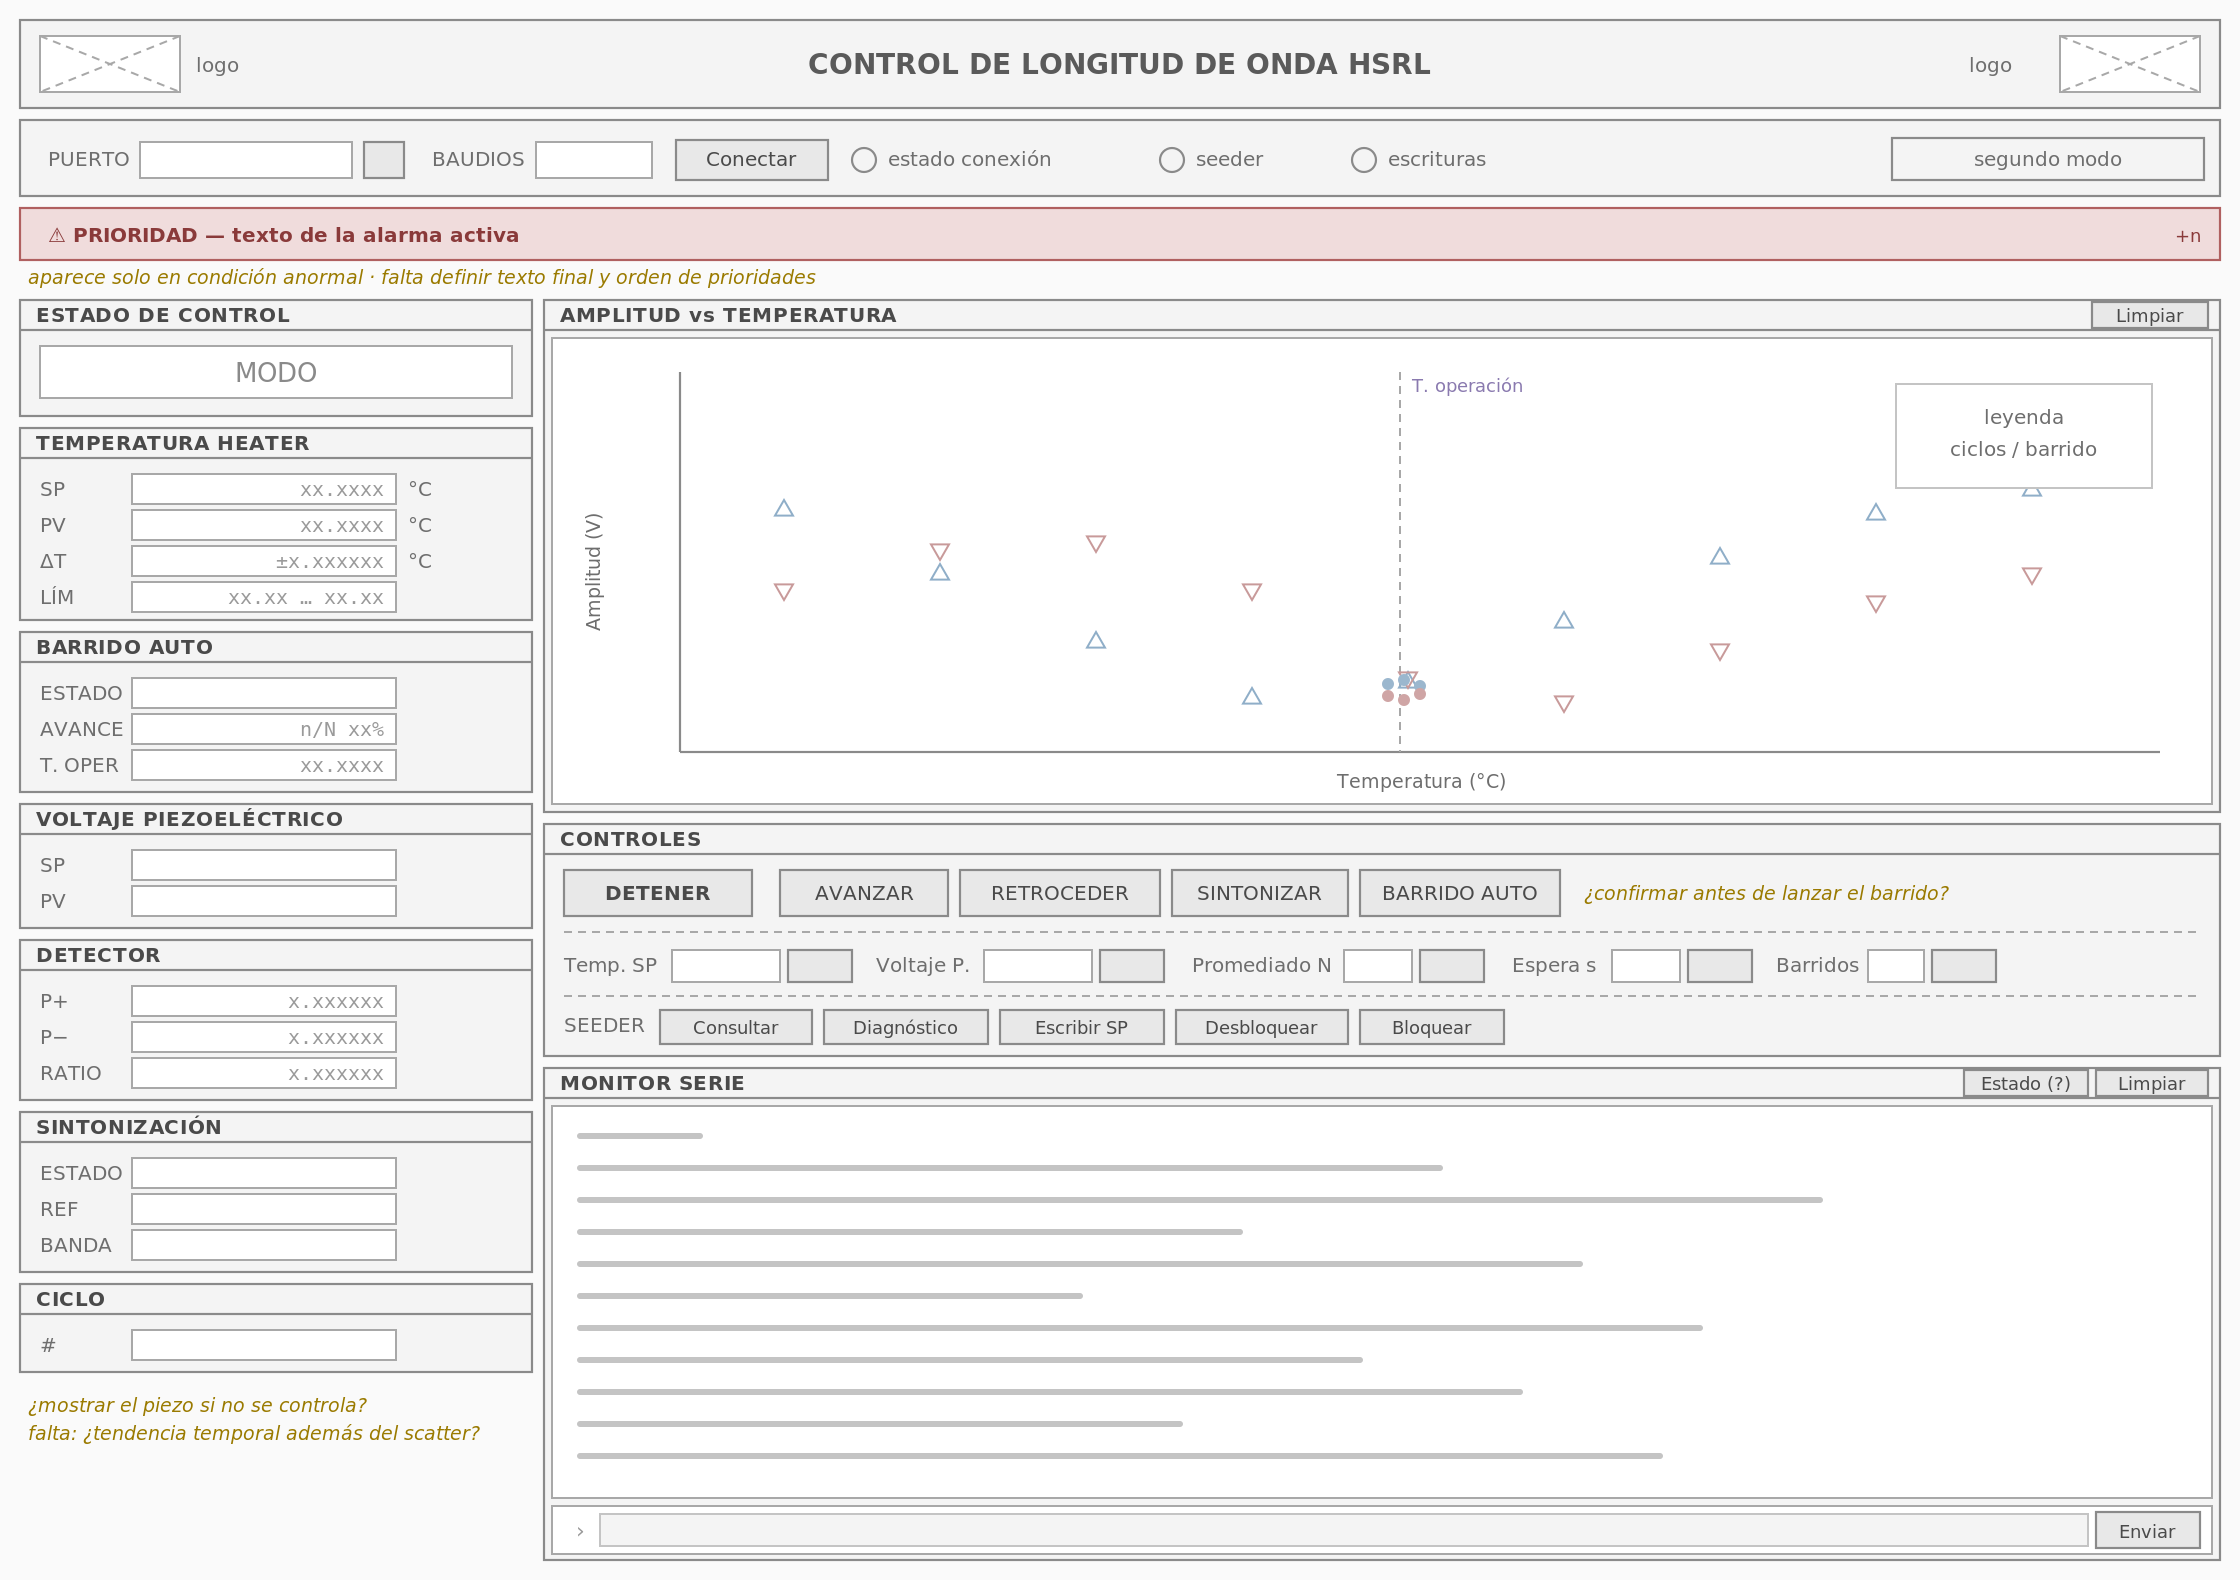
\includegraphics[width=0.8\textwidth]{figuras/8_borradorhmi.png}
    \caption{Borrador del HMI creado en Inkscape (Fuente: elaboración propia).}
    \label{fig:inks}
\end{figure}

\section{Arquitectura del software en Python}
\label{sec:arquitectura_python}
\label{sec:hmi-arquitectura}

Se implementó el HMI en Python, con Tkinter para la interfaz gráfica. El código fuente se documenta y versiona en el repositorio del proyecto. La aplicación tiene exactamente dos dependencias externas fundamentales: \texttt{pyserial} para la comunicación por puerto USB con la placa de control y \texttt{matplotlib} para la representación gráfica; Tkinter forma parte de la biblioteca estándar. Se organiza en siete módulos, según muestra la Figura~\ref{fig:hmi-modulos}.


\begin{figure}[htbp]
    \centering
    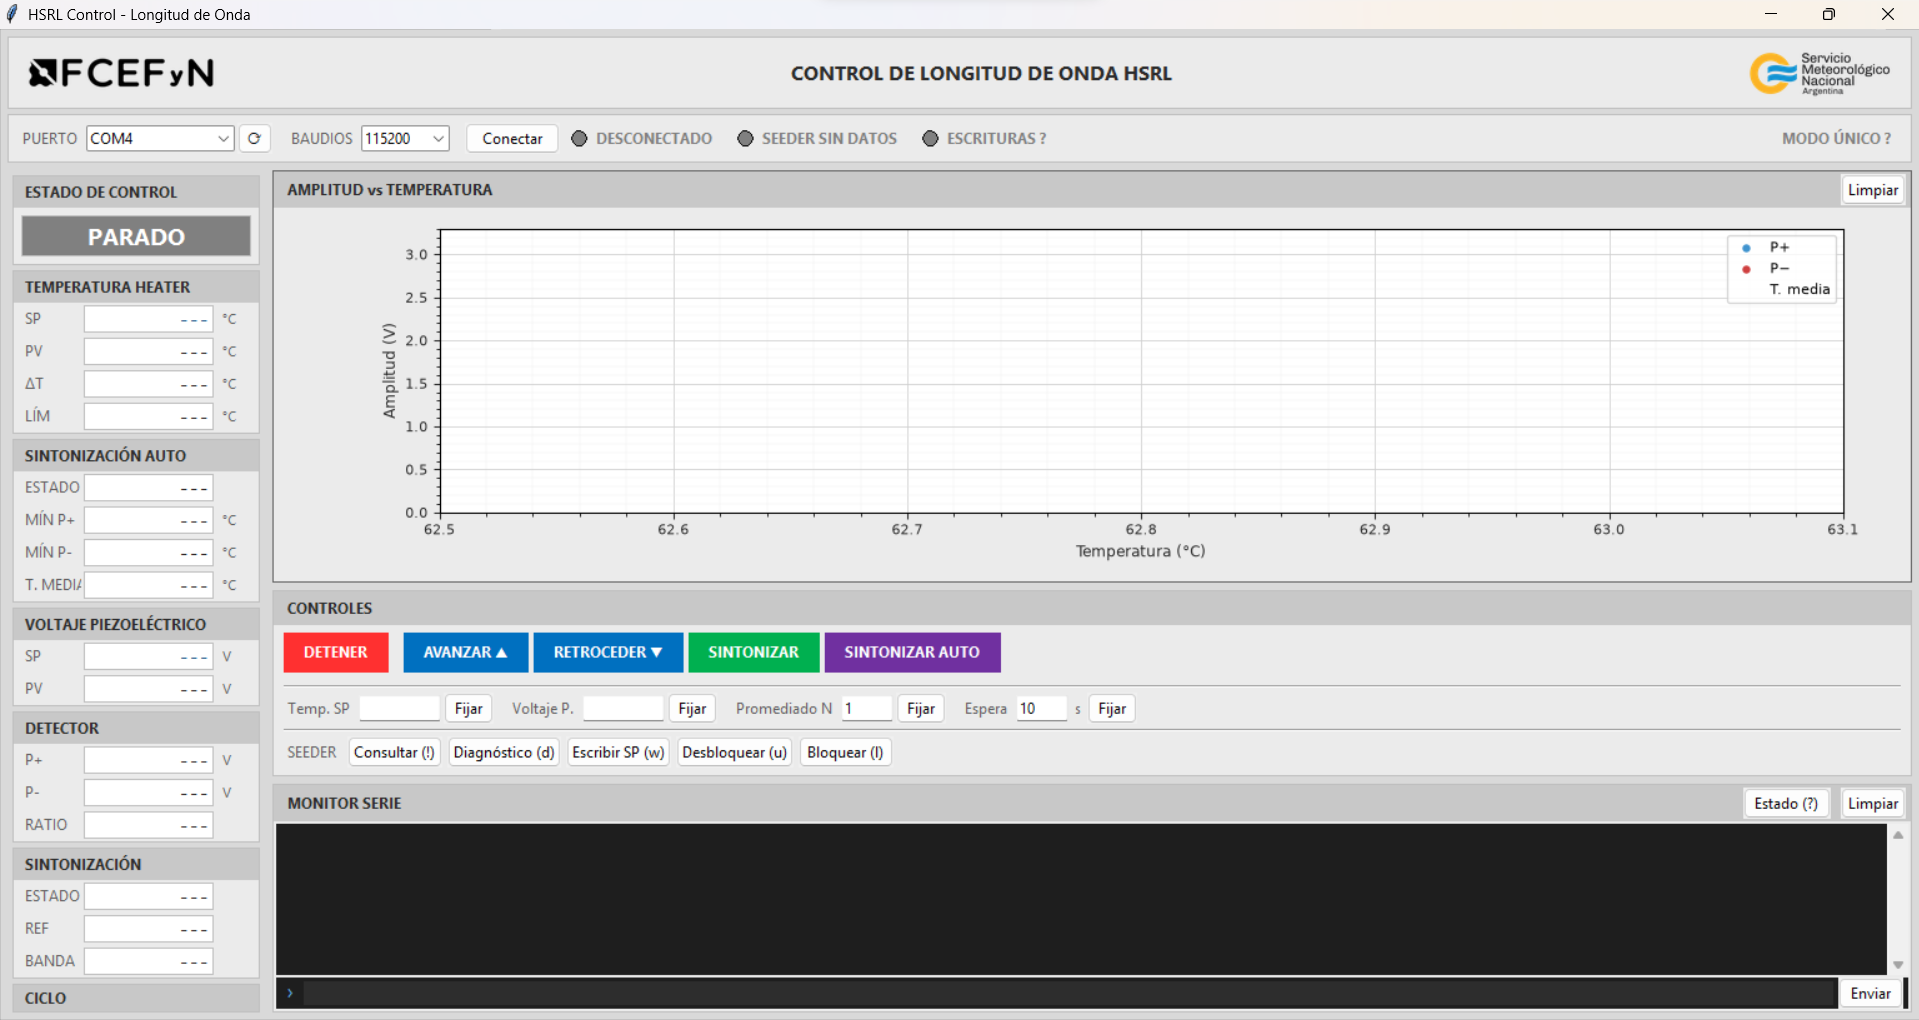
\includegraphics[width=0.8\textwidth]{figuras/8_hmilayout.png}
    \caption{HMI generado por hmi.py, a partir de la referencia proporcionada a Opus 4.7 (Fuente: elaboración propia).}
    \label{fig:hmiopus}
\end{figure}

La base de los módulos \texttt{hmi.py} y \texttt{serie.py} fueron creados a partir del uso del modelo de IA Opus 4.7, con el prompt \"crear HMI a partir de la imagen de borrador proporcionado. Cada comando de la recepción mediante pySerial debe interactuar con el firmware proporcionado con sus respectivos botones y campos de E/S\". Luego fueron modificados y adaptados según la necesidad del proyecto. Los archivos proporcionados de referencia para el modelo fueron el borrador de la Figura \ref{fig:inks} y los archivos \emph{hsrl-control.c} y \emph{config.h}.

\begin{figure}[htbp]
\centering
\resizebox{\textwidth}{!}{% Figura: hmi-modulos -- requiere % =====================================================================
%  Estilos compartidos por los diagramas TikZ de los capitulos.
%  Va en el PREAMBULO del documento principal:
%      \input{diagramas/estilos-diagramas}
% =====================================================================

\usepackage{tikz}
\usepackage{amsmath}
\usepackage{amssymb}
\usetikzlibrary{arrows.meta,positioning,shapes.geometric,shapes.misc,calc,fit,backgrounds,decorations.pathreplacing}

\definecolor{cbloque}{HTML}{E8EEF4}
\definecolor{cborde}{HTML}{4A6D8C}
\definecolor{cacento}{HTML}{D9E6D5}
\definecolor{cacentob}{HTML}{5A7A4A}
\definecolor{cgris}{HTML}{EDEDED}
\definecolor{cgrisb}{HTML}{888888}
\definecolor{calarma}{HTML}{F6DEDE}
\definecolor{calarmab}{HTML}{A03030}

\tikzset{
  bloque/.style={draw=cborde,fill=cbloque,rounded corners=2pt,align=center,
                 inner sep=5pt,font=\footnotesize,minimum height=9mm},
  bloqueg/.style={bloque,draw=cgrisb,fill=cgris},
  bloquea/.style={bloque,draw=cacentob,fill=cacento},
  bloquer/.style={bloque,draw=calarmab,fill=calarma},
  proceso/.style={bloque,minimum width=52mm},
  decision/.style={draw=cborde,fill=cbloque,align=center,font=\scriptsize,
                   diamond,aspect=2.2,inner sep=1pt},
  flecha/.style={-{Stealth[length=2mm]},draw=cborde!80!black,thick},
  flechag/.style={flecha,draw=cgrisb},
  et/.style={font=\scriptsize,inner sep=1.5pt,fill=white,align=center},
  etl/.style={et,midway},
  grupo/.style={draw=cgrisb,dashed,rounded corners=3pt,inner sep=4mm},
  tit/.style={font=\scriptsize\bfseries,text=cgrisb!60!black},
}

% --- utilidades para diagramas de secuencia ---
\tikzset{
  vida/.style={draw=cgrisb,dash pattern=on 2pt off 2pt},
  cab/.style={bloque,minimum width=26mm,font=\scriptsize\bfseries},
  nota/.style={draw=cacentob,fill=cacento,font=\scriptsize,align=center,
               rounded corners=1pt,inner sep=3pt},
}
\newcommand{\msg}[4]{\draw[flecha] (#1,#3) -- (#2,#3) node[et,midway,above=0pt]{#4};}
\newcommand{\msgr}[4]{\draw[flecha,dashed] (#1,#3) -- (#2,#3) node[et,midway,above=0pt]{#4};}
\newcommand{\auto}[3]{%
  \draw[flecha] (#1,#2) -- ++(0.55,0) -- ++(0,-0.42) -- (#1,{#2-0.42});
  \node[et,anchor=west] at ({#1+0.7},{#2-0.21}) {#3};}

 en el preambulo
\begin{tikzpicture}[x=1cm,y=1cm]

\node[bloque,text width=62mm] (hmi) at (2.0,3.2)
  {\texttt{hmi.py}\\[1pt]\scriptsize \texttt{HmiApplication}: construcción de la pantalla,
   \texttt{\_poll\_serial()} cada 100\,ms, secuencia de sintonización automática};

\node[bloque,text width=34mm] (ser) at (-5.4,0.5)
  {\texttt{serie.py}\\[1pt]\scriptsize \texttt{SerialLink}: hilo lector,\\cola de líneas, \texttt{SerialLinkError}};
\node[bloque,text width=36mm] (tel) at (-0.4,0.5)
  {\texttt{telemetria.py}\\[1pt]\scriptsize \texttt{ProcessData} + \texttt{parse\_line()}\\(no importa Tkinter)};
\node[bloque,text width=32mm] (reg) at (4.4,0.5)
  {\texttt{registro.py}\\[1pt]\scriptsize \texttt{session\_log()} y\\\texttt{CycleCsvWriter}};
\node[bloque,text width=36mm] (wid) at (9.4,0.5)
  {\texttt{widgets.py}\\[1pt]\scriptsize \texttt{StatusIndicator}, \texttt{StatusLabel},\\\texttt{group\_box()}, \texttt{value\_row()}};

\node[bloqueg,text width=32mm] (py)  at (-5.4,-2.2) {\texttt{pyserial}\\[1pt]\scriptsize puerto USB-CDC};
\node[bloquea,text width=42mm] (fw)  at (1.4,-2.2)
  {\texttt{firmware.py}\\[1pt]\scriptsize constantes espejo de \texttt{config.h} y \texttt{LOG\_COLUMNS}};
\node[bloquea,text width=36mm] (est) at (7.8,-2.2)
  {\texttt{estilo.py}\\[1pt]\scriptsize paleta ISA-101 y tipografía};

\draw[flecha] (hmi) -- (ser);
\draw[flecha] (hmi) -- (tel);
\draw[flecha] (hmi) -- (reg);
\draw[flecha] (hmi) -- (wid);
\draw[flechag] (tel) -- (fw);
\draw[flechag] (reg.south) -- ++(0,-0.9) -| (fw.30);
\draw[flechag] (wid) -- (est);
\draw[flechag] (ser) -- (py);

\node[et,anchor=north west,align=left] at (-7.4,-3.4)
  {\scriptsize $\longrightarrow$ dependencia de importación};

\end{tikzpicture}
}
\caption{Arquitectura de módulos de la interfaz de operación.}
\label{fig:hmi-modulos}
\end{figure}

\begin{table}[htbp]
\centering
\caption{Responsabilidad de cada módulo de la interfaz.}
\label{tab:hmi-modulos}
  \begin{tabular}{@{}p{0.24\textwidth}p{0.68\textwidth}@{}}
  \toprule
  \textbf{Módulo} & \textbf{Responsabilidad} \\
  \midrule
  \texttt{hmi.py} & Clase \texttt{HmiApplication}: construcción de la pantalla, ciclo de sondeo, envío de comandos y secuencia de sintonización automática. Punto de entrada. \\
  \texttt{serie.py} & Clase \texttt{SerialLink}: apertura, cierre, hilo de lectura y cola de líneas. Traduce toda falla del puerto a \texttt{SerialLinkError}. \\
  \texttt{telemetria.py} & Modelo del proceso (\texttt{ProcessData}) y análisis de las líneas de texto del firmware. \\
  \texttt{registro.py} & \texttt{session\_log()} para la traza de la sesión y \texttt{CycleCsvWriter} para el archivo CSV de ciclos. \\
  \texttt{widgets.py} & Componentes reutilizables (\texttt{StatusIndicator}, \texttt{StatusLabel}, \texttt{group\_box()}, \texttt{value\_row()}) con el estilo ya aplicado. \\
  \texttt{estilo.py} & Paleta y tipografía conforme a ISA-101. \\
  \texttt{firmware.py} & Constantes que deben coincidir con las del firmware. \\
  \bottomrule
  \end{tabular}
\end{table}

Para centralizar los datos del proceso se utiliza la clase \texttt{ProcessData}. Esta clase posee todos sus atributos declarados en el constructor, con la unidad y el significado al lado, lo que hace que el modelo del proceso se lea como una especificación de qué sabe la interfaz sobre el instrumento. La ventaja de esta aproximación es que permite probar separado el módulo \texttt{telemetria.py} del resto de la interfaz, para validar respuestas del microcontrolador sin necesidad de pasar por la interfaz HMI.

\section{Puerto serie y concurrencia}
\label{sec:hmi-concurrencia}

Tkinter impone que todo acceso a los componentes gráficos deben ocurrir desde el hilo que ejecuta el bucle de eventos (invocado por \texttt{hmi.py}). Al mismo tiempo, la lectura del puerto serie debe ser continua para no perder datos ni consumir un núcleo completo en espera activa. La estructura adoptada, ilustrada en la Figura~\ref{fig:hmi-datos}, resuelve ambas restricciones.

\begin{figure}[htbp]
\centering
\resizebox{0.7\textwidth}{!}{% Figura: hmi-datos -- requiere % =====================================================================
%  Estilos compartidos por los diagramas TikZ de los capitulos.
%  Va en el PREAMBULO del documento principal:
%      \input{diagramas/estilos-diagramas}
% =====================================================================

\usepackage{tikz}
\usepackage{amsmath}
\usepackage{amssymb}
\usetikzlibrary{arrows.meta,positioning,shapes.geometric,shapes.misc,calc,fit,backgrounds,decorations.pathreplacing}

\definecolor{cbloque}{HTML}{E8EEF4}
\definecolor{cborde}{HTML}{4A6D8C}
\definecolor{cacento}{HTML}{D9E6D5}
\definecolor{cacentob}{HTML}{5A7A4A}
\definecolor{cgris}{HTML}{EDEDED}
\definecolor{cgrisb}{HTML}{888888}
\definecolor{calarma}{HTML}{F6DEDE}
\definecolor{calarmab}{HTML}{A03030}

\tikzset{
  bloque/.style={draw=cborde,fill=cbloque,rounded corners=2pt,align=center,
                 inner sep=5pt,font=\footnotesize,minimum height=9mm},
  bloqueg/.style={bloque,draw=cgrisb,fill=cgris},
  bloquea/.style={bloque,draw=cacentob,fill=cacento},
  bloquer/.style={bloque,draw=calarmab,fill=calarma},
  proceso/.style={bloque,minimum width=52mm},
  decision/.style={draw=cborde,fill=cbloque,align=center,font=\scriptsize,
                   diamond,aspect=2.2,inner sep=1pt},
  flecha/.style={-{Stealth[length=2mm]},draw=cborde!80!black,thick},
  flechag/.style={flecha,draw=cgrisb},
  et/.style={font=\scriptsize,inner sep=1.5pt,fill=white,align=center},
  etl/.style={et,midway},
  grupo/.style={draw=cgrisb,dashed,rounded corners=3pt,inner sep=4mm},
  tit/.style={font=\scriptsize\bfseries,text=cgrisb!60!black},
}

% --- utilidades para diagramas de secuencia ---
\tikzset{
  vida/.style={draw=cgrisb,dash pattern=on 2pt off 2pt},
  cab/.style={bloque,minimum width=26mm,font=\scriptsize\bfseries},
  nota/.style={draw=cacentob,fill=cacento,font=\scriptsize,align=center,
               rounded corners=1pt,inner sep=3pt},
}
\newcommand{\msg}[4]{\draw[flecha] (#1,#3) -- (#2,#3) node[et,midway,above=0pt]{#4};}
\newcommand{\msgr}[4]{\draw[flecha,dashed] (#1,#3) -- (#2,#3) node[et,midway,above=0pt]{#4};}
\newcommand{\auto}[3]{%
  \draw[flecha] (#1,#2) -- ++(0.55,0) -- ++(0,-0.42) -- (#1,{#2-0.42});
  \node[et,anchor=west] at ({#1+0.7},{#2-0.21}) {#3};}

 en el preambulo
\begin{tikzpicture}[x=1cm,y=1cm,
  paso/.style={bloque,text width=54mm},
  dec/.style={decision,text width=30mm},
  canal/.style={draw=cborde!80!black,thick},
  banda/.style={draw=cgrisb,dashed,rounded corners=3pt,fill=cgris!45}]

% ---------------- bandas ----------------
\begin{scope}[on background layer]
  \fill[banda] (-9.6,-9.4) rectangle (11.0,2.9);
  \fill[banda] (-9.6,-35.2) rectangle (11.0,-12.4);
\end{scope}
\node[tit,anchor=north west] at (-9.5,2.8)   {hilo lector \textemdash\ \texttt{serie.py}, continuo};
\node[tit,anchor=north west] at (-9.5,-12.5) {hilo principal de Tk \textemdash\ \texttt{hmi.py}};

% ---------------- hilo lector ----------------
\node[dec]  (a1) at (0,0)    {¿hay bytes\\en el puerto?};
\node[paso] (a2) at (0,-2.4) {Leer, decodificar y acumular en el buffer};
\node[dec]  (a3) at (0,-4.8) {¿el buffer tiene\\una línea completa?};
\node[paso] (a4) at (0,-7.4) {Cortar la línea y ponerla en la cola};

\node[bloqueg,text width=30mm] (aw) at (6.4,0)  {Esperar 5\,ms};
\node[bloquer,text width=34mm] (ae) at (-6.6,-2.4)
  {Falla del puerto:\\[1pt]\scriptsize levantar \texttt{connection\_lost} y terminar el hilo};

\draw[flecha] (a1) -- node[et,right]{sí} (a2);
\draw[flecha] (a2) -- (a3);
\draw[flecha] (a3) -- node[et,right]{sí} (a4);
\draw[flecha] (a1.east) -- node[et,above]{no} (aw.west);
\draw[canal] (aw.north) -- (6.4,1.6) -- (0,1.6);
\draw[canal] (a3.west) -- node[et,above,pos=0.25]{no} (-9.1,-4.8) -- (-9.1,1.6) -- (0,1.6);
\draw[flecha] (0,1.6) -- (a1.north);
\draw[flecha] (a4.east) -- (9.6,-7.4) -- (9.6,-4.8) -- (a3.east);
\draw[flechag] (a2.west) -- node[et,above]{excepción} (ae.east);

% ---------------- la cola ----------------
\node[bloquea,text width=58mm,draw=cacentob,dashed] (q) at (0,-10.9)
  {\texttt{queue.Queue}\\[1pt]\scriptsize frontera entre los dos hilos};
\draw[flecha] (a4.south) -- (q.north);
\draw[flecha] (q.south) -- (0,-13.05);

% ---------------- hilo principal de Tk ----------------
\node[bloquea,text width=54mm] (b0) at (0,-13.8)
  {\texttt{\_poll\_serial()}\\[1pt]\scriptsize \texttt{root.after} cada 100\,ms};
\node[paso] (b1) at (0,-16.2) {Tomar de la cola hasta 50 líneas};
\node[dec]  (b2) at (0,-18.6) {¿queda alguna\\línea del lote?};
\node[paso] (b3) at (0,-21.2) {Eco en el monitor y \texttt{parse\_line()}\\[1pt]\scriptsize actualiza \texttt{ProcessData}};
\node[dec]  (b4) at (0,-23.8) {¿la línea\\cerró un ciclo?};
\node[paso,text width=58mm] (b5) at (0,-26.4)
  {\texttt{track\_minima()}, punto al gráfico, fila al CSV y paso de la sintonización automática};
\node[dec]  (b6) at (0,-29.0) {¿\texttt{connection}\\\texttt{\_lost}?};
\node[dec]  (b7) at (0,-32.2) {¿hubo\\novedades?};

\node[bloquer,text width=34mm] (bd) at (6.6,-29.0) {Avisar y cerrar el puerto};
\node[bloque,text width=34mm]  (br) at (6.6,-32.2) {\texttt{\_refresh\_display()}};

\draw[flecha] (b0) -- (b1);
\draw[flecha] (b1) -- (b2);
\draw[flecha] (b2) -- node[et,right]{sí} (b3);
\draw[flecha] (b3) -- (b4);
\draw[flecha] (b4) -- node[et,right]{sí} (b5);
\draw[canal] (b4.east) -- node[et,above,pos=0.35]{no} (9.6,-23.8);
\draw[canal] (b5.east) -- (9.6,-26.4);
\draw[canal] (9.6,-26.4) -- (9.6,-18.6);
\draw[flecha] (9.6,-18.6) -- (b2.east);
\draw[flecha] (b2.west) -- node[et,above,pos=0.22]{no} (-9.1,-18.6) -- (-9.1,-29.0) -- (b6.west);
\draw[flecha] (b6) -- node[et,left]{no} (b7);
\draw[flecha] (b6.east) -- node[et,above]{sí} (bd.west);
\draw[flecha] (b7.east) -- node[et,above]{sí} (br.west);
\draw[flechag] (bd.south) -- (6.6,-30.6) -- (0,-30.6);
\draw[flechag] (br.south) -- (6.6,-34.2) -- (0,-34.2);
\draw[flecha] (b7.south) -- node[et,left,pos=0.45]{no} (0,-34.2) -- (10.3,-34.2)
      -- node[et,pos=0.55,right,rotate=90]{\texttt{root.after(100\,ms)}} (10.3,-13.8) -- (b0.east);

\end{tikzpicture}}
\caption[Diagrama de flujo de un ciclo de \textit{log} (Fuente: elaboración propia.)]%
{Recorrido de un ciclo de telemetría desde el puerto hasta la pantalla.}
\label{fig:hmi-datos}
\end{figure}

\begin{itemize}
\item Un \textbf{hilo secundario} creado en la clase SerialLink lee del puerto, acumula los bytes en un buffer, separa las líneas completas y las deposita en una \texttt{queue.Queue}.
\item El \textbf{hilo principal} corre \texttt{\_poll\_serial()} cada $100$\,ms, con \texttt{root.after()}. Este hilo lee la cola de lineas completas, la vacía y actualiza la interfaz gráfica.
\end{itemize}

Para la implementación, se debió tener en cuenta ciertos detalles que se volvieron críticos al funcionamiento de la misma.

La función \texttt{pending\_lines()} devuelve como máximo 50 líneas por llamada. Sin ese límite, un firmware que emita más rápido de lo que la pantalla puede dibujar mantiene al hilo principal vaciando la cola de forma indefinida. En consecuencia la interfaz deja de responder.

Cuando no hay bytes disponibles, el hilo secundario duerme $5$\,ms y cuando directamente no hay puerto abierto, la pausa sube a $50$\,ms. Esta implementación es para evitar consumir recursos innecesariamente cuando no existan datos por leer.

Si el enlace por puerto serie se corta por sí solo debido a un cable desconectado o microcontrolador reiniciado el hilo lector levanta una bandera, \texttt{connection\_lost}, que el hilo principal consulta después de vaciar la cola. El hilo distingue además el cierre solicitado del inesperado, esto es, si el cierre fue pedido por el operador o no, y genera una excepción acorde.

Finalmente, todas las fallas de \texttt{pyserial} se traducen dentro de \texttt{serie.py} a una excepción propia, \texttt{SerialLinkError} 

\section{Lectura de datos del proceso}
\label{sec:hmi-telemetria}

Como se estableció en la Sección~\ref{sec:fw-log}, el firmware envía al finalizar un ciclo de medición una línea \texttt{[log]} autocontenida, y anuncia los nombres de sus columnas por separado en \texttt{[logcols]}. La interfaz se apoya íntegramente en estos dos mecanismos y por lo tanto el estado del proceso se reconstruye a partir de esa única línea.

El análisis ocurre en dos etapas. La primera asocia por posición los nombres anunciados en \texttt{[logcols]} con los valores de la línea \texttt{[log]}, y construye un diccionario de nombre a texto; la segunda lee de ese diccionario los campos que la interfaz necesita:

\begin{lstlisting}[language=Python,basicstyle=\ttfamily\footnotesize,
  columns=fullflexible,breaklines=true,frame=single,rulecolor=\color{black!30}]
fields = {}
values = data.log_row_raw.split(",")
for i in range(len(data.log_columns)):
    if i < len(values):
        fields[data.log_columns[i]] = values[i].strip()

data.cycle_number    = _to_int(fields.get("ciclo", ""), data.cycle_number)
data.heater_setpoint = _to_float(fields.get("heater_sp", ""), data.heater_setpoint)
data.heater_measured = _to_float(fields.get("heater_real", ""), data.heater_measured)
...
data.lock_active     = _to_bool(fields.get("lock_activo", ""), data.lock_active)
\end{lstlisting}

La separación en dos etapas hace que el resto de la función no dependa del orden de las columnas, y de ahí se consigue que el firmware puede agregar columnas sin romper la interfaz. La asociación de los datos con el nombre de las columnas siempre es por nombre, no por orden.

Las respuestas a comandos puntuales tales como consulta al seeder, diagnóstico, bloqueo y desbloqueo, verificación de escritura o ecos de \texttt{A} y \texttt{E} no forman parte del ciclo y llegan como texto libre. La función \texttt{parse\_line()} las resuelve como condiciones excluyentes, cada una con su retorno inmediato:

\begin{lstlisting}[language=Python,basicstyle=\ttfamily\footnotesize,
  columns=fullflexible,breaklines=true,frame=single,rulecolor=\color{black!30}]
def parse_line(line, data):
    rest = _text_after(line, "[logcols]")
    if rest is not None:
        data.log_columns = [name.strip() for name in rest.split(",")]
        return True

    rest = _text_after(line, "[log]")
    if rest is not None:
        _update_from_log(data, rest)
        return True

    if "muestras a promediar" in line:
        data.averaging_samples = _to_int(_first_word(_value_after_equals(line)),
                                         data.averaging_samples)
        return True
    ...
    return False
\end{lstlisting}

\subsection{La clase \texttt{ProcessData}}

\texttt{ProcessData} concentra el estado completo del proceso. Además de los campos que provienen directamente de la telemetría, incorpora tres funciones que merecen mención.

El primero es el seguimiento de mínimos, en \texttt{track\_minima()}. Mientras el sistema barre en temperatura, la interfaz conserva el valor mínimo de cada canal y la temperatura a la que ocurrió. El firmware no registra nada de esto, de modo que la interfaz es su única fuente. El cálculo de mínimo tiene en cuenta el valor de temperatura anterior al último, puesto que el set point actual siempre corresponde al proximo ciclo.

\begin{lstlisting}[language=Python,basicstyle=\ttfamily\footnotesize,
  columns=fullflexible,breaklines=true,frame=single,rulecolor=\color{black!30}]
measured_at = self.heater_setpoint - self.heater_step   # temperatura de esta medicion

if self.min_p_plus == 0.0 or self.p_plus < self.min_p_plus:
    self.min_p_plus = self.p_plus
    self.temp_at_min_p_plus = measured_at
\end{lstlisting}

Sólo se consideran los ciclos de barrido, y el modo de detención borra lo registrado para evitar arrastrar los mínimos de un intento anterior, posiblemente realizado en otras condiciones.

El segundo es \texttt{plot\_temperature()}, la selección de la temperatura para el eje de abscisas del gráfico. Se prefiere la temperatura medida por el seeder; si el seeder no responde, esa lectura llega como cero y se utiliza en su lugar el setpoint, que sigue siendo un dato válido. La pantalla informa cuál de las dos está en uso.

El tercero es \texttt{clear\_seeder\_state()}, que vuelve la interfaz a los valores de inicio y se invoca al cerrar el puerto. Sin puerto no hay forma de saber en qué condición está el seeder, y dejar los indicadores mostrando la última lectura conocida equivaldría a afirmar algo que ya no es correcto. 


\subsection{Representación gráfica de valores medidos}

El gráfico central de puntos de dispersión presenta $P_{+}$ y $P_{-}$ en función de la temperatura, con un punto por ciclo y una ventana móvil de los últimos $500$ ciclos. La elección de la temperatura como abscisa responde a que la magnitud de interés durante la sintonización es precisamente la dependencia de las amplitudes con la temperatura, y en esa representación los mínimos de ambos canales resultan visibles de forma directa. Una línea vertical punteada marca el punto medio entre los mínimos registrados.

Ambos ejes tienen límites fijos; el eje de ordenadas cubre el rango completo del conversor del microcontrolador, de $0$ a $3{,}3$\,V y el de abscisas cubre el rango de seguridad del calefactor, $[h_{\min}, h_{\max}]$.

El costo de la decisión es que los puntos fuera del rango de seguridad no se dibujan. Se acepta porque el firmware no permite que el punto de consigna permanezca fuera de ese rango: la protección descripta en la Sección~\ref{sec:fw-control} lo devuelve al lugar seguro, de modo que un dato fuera del eje corresponde a una condición transitoria que la banda de alarmas ya señala.


\section{Gestión de alarmas}
\label{sec:hmi-alarmas}

La interfaz gestiona cinco condiciones anormales, cuya evaluación y selección se ilustra en la Figura~\ref{fig:hmi-alarmas} y se detalla en la Tabla~\ref{tab:hmi-alarmas}.

\begin{figure}[htbp]
\centering
\resizebox{\textwidth}{!}{% Figura: hmi-alarmas -- requiere % =====================================================================
%  Estilos compartidos por los diagramas TikZ de los capitulos.
%  Va en el PREAMBULO del documento principal:
%      \input{diagramas/estilos-diagramas}
% =====================================================================

\usepackage{tikz}
\usepackage{amsmath}
\usepackage{amssymb}
\usetikzlibrary{arrows.meta,positioning,shapes.geometric,shapes.misc,calc,fit,backgrounds,decorations.pathreplacing}

\definecolor{cbloque}{HTML}{E8EEF4}
\definecolor{cborde}{HTML}{4A6D8C}
\definecolor{cacento}{HTML}{D9E6D5}
\definecolor{cacentob}{HTML}{5A7A4A}
\definecolor{cgris}{HTML}{EDEDED}
\definecolor{cgrisb}{HTML}{888888}
\definecolor{calarma}{HTML}{F6DEDE}
\definecolor{calarmab}{HTML}{A03030}

\tikzset{
  bloque/.style={draw=cborde,fill=cbloque,rounded corners=2pt,align=center,
                 inner sep=5pt,font=\footnotesize,minimum height=9mm},
  bloqueg/.style={bloque,draw=cgrisb,fill=cgris},
  bloquea/.style={bloque,draw=cacentob,fill=cacento},
  bloquer/.style={bloque,draw=calarmab,fill=calarma},
  proceso/.style={bloque,minimum width=52mm},
  decision/.style={draw=cborde,fill=cbloque,align=center,font=\scriptsize,
                   diamond,aspect=2.2,inner sep=1pt},
  flecha/.style={-{Stealth[length=2mm]},draw=cborde!80!black,thick},
  flechag/.style={flecha,draw=cgrisb},
  et/.style={font=\scriptsize,inner sep=1.5pt,fill=white,align=center},
  etl/.style={et,midway},
  grupo/.style={draw=cgrisb,dashed,rounded corners=3pt,inner sep=4mm},
  tit/.style={font=\scriptsize\bfseries,text=cgrisb!60!black},
}

% --- utilidades para diagramas de secuencia ---
\tikzset{
  vida/.style={draw=cgrisb,dash pattern=on 2pt off 2pt},
  cab/.style={bloque,minimum width=26mm,font=\scriptsize\bfseries},
  nota/.style={draw=cacentob,fill=cacento,font=\scriptsize,align=center,
               rounded corners=1pt,inner sep=3pt},
}
\newcommand{\msg}[4]{\draw[flecha] (#1,#3) -- (#2,#3) node[et,midway,above=0pt]{#4};}
\newcommand{\msgr}[4]{\draw[flecha,dashed] (#1,#3) -- (#2,#3) node[et,midway,above=0pt]{#4};}
\newcommand{\auto}[3]{%
  \draw[flecha] (#1,#2) -- ++(0.55,0) -- ++(0,-0.42) -- (#1,{#2-0.42});
  \node[et,anchor=west] at ({#1+0.7},{#2-0.21}) {#3};}

 en el preambulo
\begin{tikzpicture}[x=1cm,y=1cm]

\node[bloque,text width=44mm] (est) at (0,0) {Estado del proceso\\\scriptsize (\texttt{ProcessData} tras cada ciclo)};

\node[bloquer,text width=60mm] (a1) at (7.8,2.6)
  {\textbf{ALTA} — Segundo modo detectado\\[1pt]\scriptsize \texttt{second\_mode\_alarm}: la medición no es confiable};
\node[bloquer,text width=60mm] (a2) at (7.8,1.0)
  {\textbf{ALTA} — Temperatura fuera de límites\\[1pt]\scriptsize \texttt{heater\_alarm\_priority()} $=$ \texttt{ALARM\_HIGH}};
\node[bloque,text width=60mm] (a3) at (7.8,-0.6)
  {\textbf{MEDIA} — Temperatura cerca del límite\\[1pt]\scriptsize 5\,\% final del rango};
\node[bloque,text width=60mm] (a4) at (7.8,-2.2)
  {\textbf{MEDIA} — Escrituras protegidas\\[1pt]\scriptsize \texttt{writes\_enabled is False}: usar Desbloquear (\texttt{u})};
\node[bloque,text width=60mm] (a5) at (7.8,-3.8)
  {\textbf{MEDIA} — Seeder sin respuesta\\[1pt]\scriptsize \texttt{seeder\_responding is False}};

\node[bloque,text width=40mm] (ord) at (15.8,-0.6)
  {Filtrar las activas\\y ordenar por prioridad\\[1pt]\scriptsize \texttt{ALARM\_HIGH} $=0$, \texttt{ALARM\_MEDIUM} $=1$};
\node[decision,text width=22mm] (vac) at (15.8,-3.6) {¿lista\\vacía?};
\node[bloqueg,text width=34mm] (oc) at (11.8,-5.9) {Ocultar la banda};
\node[bloquea,text width=48mm] (mo) at (18.4,-5.9)
  {Mostrar la de mayor prioridad:\\[1pt]\scriptsize prioridad + qué pasa + qué hacer,\\ con el contador ``$+n$ más''};

\foreach \n in {a1,a2,a3,a4,a5}{\draw[flechag] (est) -- (\n.west);}
\foreach \n in {a1,a2,a3,a4,a5}{\draw[flechag] (\n.east) -- (ord.west);}
\draw[flecha] (ord) -- (vac);
\draw[flecha] (vac) -| node[et,pos=0.25,above]{sí} (oc);
\draw[flecha] (vac) -| node[et,pos=0.25,above]{no} (mo);

\node[nota,text width=82mm,anchor=north west] at (0,-7.2)
 {\texttt{heater\_alarm\_priority()} es una función pura y la única fuente del criterio de temperatura:
  la usan tanto el indicador del panel como la banda de alarmas, de modo que no pueden
  discrepar. El color es redundante con el texto, nunca la única pista (ISA-18.2).};

\end{tikzpicture}
}
\caption{Evaluación y selección de la alarma presentada en la banda.}
\label{fig:hmi-alarmas}
\end{figure}

\begin{table}[htbp]
\centering
\caption{Alarmas gestionadas por la interfaz.}
\label{tab:hmi-alarmas}
  \begin{tabular}{@{}p{0.26\textwidth}cp{0.52\textwidth}@{}}
  \toprule
  \textbf{Alarma} & \textbf{Prioridad} & \textbf{Significado} \\
  \midrule
  Segundo modo detectado & Alta & El seeder abandonó la operación en modo único; la medición del ciclo no es confiable. \\
  Temperatura fuera de límites & Alta & La temperatura medida quedó fuera del rango que declara el firmware. \\
  Temperatura cerca del límite & Media & La temperatura ingresó en el $5\%$ final del rango. \\
  Escrituras protegidas & Media & El seeder ignora los puntos de consigna; requiere desbloqueo. \\
  Seeder sin respuesta & Media & No hay lectura real de temperatura ni de tensión del piezoeléctrico. \\
  \bottomrule
  \end{tabular}
\end{table}

Las alarmas activas se ordenan por prioridad y se presenta únicamente la de mayor jerarquía, acompañada de un contador de las restantes. Presentarlas todas simultáneamente reproduciría el problema que la norma busca evitar: una pantalla saturada de avisos en la que el operador deja de distinguir el importante. La banda se oculta por completo cuando no hay condiciones activas, de modo que su sola aparición ya constituye información.

El mensaje de la alarma de escrituras protegidas, por ejemplo, no se limita a nombrar la condición sino que indica la acción correctiva: \emph{«el seeder ignora los setpoints, usar Desbloquear (u)»}. El color refuerza el mensaje pero no lo reemplaza; la pantalla es legible en escala de grises.

 La evaluación de la alarma de temperatura se implementa como una función pura, \texttt{heater\_alarm\_priority(data)}, que devuelve la prioridad o \texttt{None}. Esa misma función alimenta tanto el coloreado del indicador en el panel como la banda de alarmas. Duplicar el criterio en dos lugares habría abierto la posibilidad de que el panel y la banda discrepen tras una modificación, situación particularmente perniciosa porque destruye la confianza del operador en la pantalla.

Además de la banda, la barra superior presenta cuatro indicadores permanentes ---enlace USB, enlace con el seeder, estado de las escrituras y modo único--- cada uno con tres estados posibles, incluido el estado «sin dato». La distinción entre «sin dato» y «normal» evita que la pantalla afirme normalidad cuando en realidad no ha recibido información.

\section{Sintonización automática}
\label{sec:hmi-auto}

\subsection{Fundamento}

La búsqueda del punto de operación descripta en la Sección~\ref{sec:fw-principio} es un procedimiento de varios pasos que el operador puede ejecutar a mano. Automatizarlo reduce el tiempo de puesta en marcha y elimina una fuente de error, pero plantea la cuestión de dónde implementarlo.

La decisión fue implementarlo en la interfaz y no en el firmware, por dos razones. La primera es que la secuencia es una \emph{política} y no un \emph{mecanismo}: depende de criterios que pueden ajustarse con la experiencia de operación, y modificarla no debería requerir recompilar y reprogramar el microcontrolador. La segunda es que la secuencia se construye enteramente con comandos que el firmware ya expone, de modo que su implementación en la interfaz no agrega superficie de falla al componente crítico.

\subsection{Desarrollo de la secuencia}

El diagrama de flujo de la Figura~\ref{fig:hmi-auto} detalla la secuencia completa, incluidas sus condiciones de rechazo. Mientras el sistema barre, la interfaz sigue los mínimos de cada canal y muestra en vivo la temperatura media resultante. Al activarse la sintonización automática:

\begin{enumerate}
\item Se envía \texttt{s} para que el calefactor deje de barrer. Sin este paso, el ciclo siguiente sumaría el paso grueso y el sistema se desplazaría del punto buscado.
\item Se envían \texttt{T} con la temperatura media y \texttt{w}. El segundo comando fuerza la escritura inmediata al seeder, sin esperar a que el microcontrolador concluya el ciclo en curso, que podría estar en medio de una pausa de estabilización de varios segundos.
\item Se aguardan $20$\,s de estabilización térmica (\texttt{AUTO\_SETTLE\_TIME\_S}).
\item Se dejan transcurrir cuatro ciclos con el calefactor quieto; la cantidad la fija la constante \texttt{AUTO\_MEASURE\_CYCLES}.
\item Se envía \texttt{g}. Como el enganche toma su referencia del cociente de dos ciclos atrás, a esa altura la referencia corresponde a una medición ya estabilizada.
\end{enumerate}

\begin{figure}[htbp]
\centering
\resizebox{\textwidth}{!}{% Figura: hmi-auto -- requiere % =====================================================================
%  Estilos compartidos por los diagramas TikZ de los capitulos.
%  Va en el PREAMBULO del documento principal:
%      \input{diagramas/estilos-diagramas}
% =====================================================================

\usepackage{tikz}
\usepackage{amsmath}
\usepackage{amssymb}
\usetikzlibrary{arrows.meta,positioning,shapes.geometric,shapes.misc,calc,fit,backgrounds,decorations.pathreplacing}

\definecolor{cbloque}{HTML}{E8EEF4}
\definecolor{cborde}{HTML}{4A6D8C}
\definecolor{cacento}{HTML}{D9E6D5}
\definecolor{cacentob}{HTML}{5A7A4A}
\definecolor{cgris}{HTML}{EDEDED}
\definecolor{cgrisb}{HTML}{888888}
\definecolor{calarma}{HTML}{F6DEDE}
\definecolor{calarmab}{HTML}{A03030}

\tikzset{
  bloque/.style={draw=cborde,fill=cbloque,rounded corners=2pt,align=center,
                 inner sep=5pt,font=\footnotesize,minimum height=9mm},
  bloqueg/.style={bloque,draw=cgrisb,fill=cgris},
  bloquea/.style={bloque,draw=cacentob,fill=cacento},
  bloquer/.style={bloque,draw=calarmab,fill=calarma},
  proceso/.style={bloque,minimum width=52mm},
  decision/.style={draw=cborde,fill=cbloque,align=center,font=\scriptsize,
                   diamond,aspect=2.2,inner sep=1pt},
  flecha/.style={-{Stealth[length=2mm]},draw=cborde!80!black,thick},
  flechag/.style={flecha,draw=cgrisb},
  et/.style={font=\scriptsize,inner sep=1.5pt,fill=white,align=center},
  etl/.style={et,midway},
  grupo/.style={draw=cgrisb,dashed,rounded corners=3pt,inner sep=4mm},
  tit/.style={font=\scriptsize\bfseries,text=cgrisb!60!black},
}

% --- utilidades para diagramas de secuencia ---
\tikzset{
  vida/.style={draw=cgrisb,dash pattern=on 2pt off 2pt},
  cab/.style={bloque,minimum width=26mm,font=\scriptsize\bfseries},
  nota/.style={draw=cacentob,fill=cacento,font=\scriptsize,align=center,
               rounded corners=1pt,inner sep=3pt},
}
\newcommand{\msg}[4]{\draw[flecha] (#1,#3) -- (#2,#3) node[et,midway,above=0pt]{#4};}
\newcommand{\msgr}[4]{\draw[flecha,dashed] (#1,#3) -- (#2,#3) node[et,midway,above=0pt]{#4};}
\newcommand{\auto}[3]{%
  \draw[flecha] (#1,#2) -- ++(0.55,0) -- ++(0,-0.42) -- (#1,{#2-0.42});
  \node[et,anchor=west] at ({#1+0.7},{#2-0.21}) {#3};}

 en el preambulo
\begin{tikzpicture}[x=1cm,y=1cm,
  conector/.style={draw=cborde,fill=cbloque,circle,minimum size=7mm,
                   inner sep=0pt,font=\footnotesize\bfseries}]

% ---------------- columna A: validación y puesta en el punto medio ----------------
\node[bloquea,text width=44mm] (a1) at (0,0)
  {\textbf{SINTONIZAR AUTO}\\[1pt]\scriptsize el operador presiona el botón};
\node[decision,text width=24mm] (a2) at (0,-1.8) {¿puerto\\abierto?};
\node[bloque,text width=48mm]  (a3) at (0,-3.6)
  {$t \leftarrow \dfrac{t_{\min P_{+}} + t_{\min P_{-}}}{2}$};
\node[decision,text width=26mm] (a4) at (0,-5.5) {¿hay mínimos\\registrados?};
\node[decision,text width=26mm] (a5) at (0,-7.5) {$t\in[h_{\min},h_{\max}]$?};
\node[bloque,text width=48mm]  (a6) at (0,-9.4)
  {Enviar \texttt{s}\\[1pt]\scriptsize el heater deja de barrer};
\node[bloque,text width=48mm]  (a7) at (0,-10.9)
  {Enviar \texttt{T<t>} y \texttt{w}\\[1pt]\scriptsize el setpoint entra sin esperar al ciclo en curso};
\node[bloque,text width=48mm]  (a8) at (0,-12.5)
  {Esperar \texttt{AUTO\_SETTLE\_TIME\_S} $=20$\,s\\[1pt]\scriptsize estabilización térmica};
\node[conector] (ca) at (0,-14.0) {A};

% salidas por rechazo
\node[bloquer,text width=40mm] (f1) at (-7.2,-1.8)
  {\scriptsize Mensaje \emph{No conectado} en el monitor serie};
\node[bloquer,text width=40mm] (f2) at (-7.2,-5.5)
  {\scriptsize Estado \textbf{SIN MÍNIMOS}: barrer con AVANZAR o RETROCEDER primero};
\node[bloquer,text width=40mm] (f3) at (-7.2,-7.5)
  {\scriptsize Estado \textbf{FUERA DE RANGO}: la temperatura media cae fuera de los límites};

\draw[flecha] (a1) -- (a2);
\draw[flecha] (a2) -- node[et,right]{sí} (a3);
\draw[flecha] (a3) -- (a4);
\draw[flecha] (a4) -- node[et,right]{sí} (a5);
\draw[flecha] (a5) -- node[et,right]{sí} (a6);
\draw[flecha] (a6) -- (a7);
\draw[flecha] (a7) -- (a8);
\draw[flecha] (a8) -- (ca);
\draw[flecha] (a2) -- node[et,above]{no} (f1);
\draw[flecha] (a4) -- node[et,above]{no} (f2);
\draw[flecha] (a5) -- node[et,above]{no} (f3);

% ---------------- columna B: medición y enganche ----------------
\node[conector] (cb) at (9.2,-0.7) {A};
\node[bloque,text width=48mm] (b1) at (9.2,-2.2)
  {\texttt{auto\_cycles\_left} $\leftarrow$ \texttt{AUTO\_MEASURE\_CYCLES} $=4$};
\node[bloque,text width=48mm] (b2) at (9.2,-4.0)
  {Esperar el cierre de un ciclo\\[1pt]\scriptsize línea \texttt{[log]} del firmware};
\node[bloque,text width=48mm] (b3) at (9.2,-5.6)
  {\texttt{auto\_cycles\_left} $\leftarrow$ \texttt{auto\_cycles\_left} $-\,1$};
\node[decision,text width=24mm] (b4) at (9.2,-7.5) {\texttt{auto\_cycles}\\\texttt{\_left} $>0$?};
\node[bloque,text width=54mm] (b5) at (9.2,-9.6)
  {Enviar \texttt{g}\\[1pt]\scriptsize el lock toma como referencia el $\mathit{prt}$ de dos ciclos atrás, ya estabilizado};
\node[bloquea,text width=44mm] (b6) at (9.2,-11.5)
  {\textbf{SINTONIZADO}};

\draw[flecha] (cb) -- (b1);
\draw[flecha] (b1) -- (b2);
\draw[flecha] (b2) -- (b3);
\draw[flecha] (b3) -- (b4);
\draw[flecha] (b4) -- node[et,right]{no} (b5);
\draw[flecha] (b5) -- (b6);
\draw[flecha] (b4.east) -- node[et,pos=0.28,above]{sí} (13.4,-7.5) -- (13.4,-4.0) -- (b2.east);

% ---------------- notas ----------------
\node[nota,text width=58mm,anchor=north west] at (-9.7,2.5)
 {\textbf{Precondición.} Durante el barrido con \texttt{f} o \texttt{b} el HMI sigue
  ciclo a ciclo los mínimos de $p^{+}$ y $p^{-}$ y la temperatura a la que ocurren.
  DETENER (\texttt{s}) los borra.};

\node[nota,text width=62mm,anchor=north west] at (3.6,-12.6)
 {\textbf{Cancelación.} En cualquier punto, un comando de \texttt{INTERRUPTING\_COMMANDS}
  (\texttt{s}, \texttt{f}, \texttt{b}, \texttt{g}, \texttt{e}, \texttt{T}), un botón de
  modo o la caída del puerto cancelan la secuencia.};

\end{tikzpicture}
}
\caption[Diagrama de flujo de la sintonización automática]%
{Diagrama de flujo de la secuencia de sintonización automática. Todos los comandos enviados son comandos que el operador puede emitir manualmente.}
\label{fig:hmi-auto}
\end{figure}

Los pasos 3 y 4 encadenan dos mecanismos distintos de temporización: el primero es un temporizador de la interfaz gráfica, y el segundo un contador de ciclos cerrados que se decrementa con cada línea \texttt{[log]}. La combinación es intencional: la espera de estabilización es un intervalo de tiempo físico, mientras que la cantidad de ciclos a descartar depende del ritmo del firmware, que a su vez depende de parámetros que el operador puede haber modificado.

\subsection{Condiciones de rechazo y cancelación}

La secuencia no se inicia si no hay mínimos registrados o si la temperatura media cae fuera del rango declarado por el firmware. En ambos casos no se envía ningún comando y el motivo aparece en la traza. La validación se realiza en la interfaz aun cuando el firmware también rechazaría el valor, porque un rechazo local produce un mensaje comprensible de inmediato, mientras que el rechazo remoto se manifiesta como un código de error del seeder varios segundos después.

Una vez iniciada, cualquier comando que compita con la secuencia la cancela: los botones de modo, la fijación manual del punto de consigna, o los caracteres de \texttt{INTERRUPTING\_COMMANDS} (\texttt{s}, \texttt{f}, \texttt{b}, \texttt{g}, \texttt{e} y \texttt{T}) tipeados en la traza. La cancelación no revierte lo ya enviado ---eso exigiría que la interfaz mantuviera un modelo del estado del firmware, con el riesgo consiguiente de que ambos diverjan---, sino que simplemente interrumpe el envío de los pasos restantes. En consecuencia, si la secuencia se cancela o la interfaz se cierra a mitad de camino, el microcontrolador queda en el último modo que recibió: detenido si estaba estabilizando, enganchado si ya alcanzó el paso final. Este comportamiento es predecible y verificable, que es exactamente lo que se requiere de un modo de falla.

\section{Registro de la sesión}
\label{sec:hmi-registro}

Cada ejecución genera dos archivos en el directorio \texttt{logs/}, ambos nombrados con la misma marca temporal de arranque para poder cruzarlos:

\begin{itemize}
\item \texttt{hsrl-AAAA-MM-DD\_hh-mm-ss.log}: traza completa de la sesión, incluidos los comandos enviados, las líneas recibidas y los mensajes de la propia interfaz. Su destinatario es el análisis de incidentes.
\item \texttt{hsrl-AAAA-MM-DD\_hh-mm-ss.csv}: una fila por ciclo de control. Su destinatario es el análisis de los datos.
\end{itemize}

El archivo CSV se construye respetando estrictamente el contrato de la Sección~\ref{sec:fw-log}: la interfaz antepone la marca temporal y escribe a continuación el contenido de la línea \texttt{[log]} tal como llegó, sin reformatear ni recalcular. El encabezado se toma de los nombres que el firmware anunció en \texttt{[logcols]}; sólo si la interfaz se conectó tarde y no presenció el anuncio se recurre a la lista por defecto de \texttt{firmware.py}. La consecuencia es que un cambio de columnas en el firmware se propaga al archivo sin modificar el módulo de registro.

Dos detalles de implementación responden a requisitos operativos concretos. El archivo CSV se crea recién con la primera fila, de manera que abrir la interfaz sin conectar no deja archivos vacíos acumulándose en el directorio. Y cada fila se vuelca a disco inmediatamente después de escribirse: si el programa se interrumpe, no se pierden los ciclos ya registrados. El costo en rendimiento es irrelevante frente a la cadencia del proceso, del orden de un ciclo cada decenas de segundos.

Los dos archivos se escriben con estrategias deliberadamente distintas. El CSV mantiene el descriptor abierto durante toda la sesión, porque recibe una fila cada varios segundos y volver a abrirlo cada vez sería un desperdicio. La traza de texto, en cambio, se abre y se cierra en cada línea, dentro de \texttt{session\_log()}. Esa elección tiene dos ventajas que compensan el costo: el archivo queda íntegro aunque el proceso termine de forma abrupta ---sin oportunidad de cerrar nada--- y puede leerse desde otro programa mientras la sesión está en curso, cosa que en Windows no siempre es posible con un descriptor abierto en modo exclusivo.

\paragraph{Sin acoplamiento de retorno.} Ninguno de los dos módulos de registro conoce la interfaz. \texttt{session\_log()} descarta silenciosamente los errores de escritura, porque un disco lleno no debe impedir que el operador siga controlando el instrumento. \texttt{CycleCsvWriter.append\_cycle()}, que sí tiene algo que informar ---dónde se está guardando el archivo, o por qué falló---, no recibe una función de aviso ni importa nada de Tkinter: \emph{devuelve} el par (mensaje, categoría), y es \texttt{hmi.py} quien decide mostrarlo. Invertir la dependencia de esa manera deja al módulo de registro tan verificable como \texttt{telemetria.py}, y evita el patrón, frágil, de una capa de datos que llama hacia arriba a la capa de presentación.
% =============================================================
% Capitulo 9 - Descripcion del modelo experimental
% =============================================================
\chapter{Descripción del modelo experimental}
\label{cap:modelo_experimental}

En los capítulos precedentes se desarrollaron por separado el circuito de detección de picos, la selección del microcontrolador, el diseño del circuito impreso, el \emph{firmware} embebido y el software de supervisión. El presente capítulo describe el conjunto ya integrado y en condiciones de operación: cómo quedó montado el modelo sobre el instrumento, qué funciones expone al operador, cuál es el procedimiento de puesta en marcha, qué ensayos se realizaron sobre el sistema HSRL del Observatorio de Pilar y qué limitaciones conserva el prototipo.

\section{Integración del sistema}
\label{sec:me-integracion}

El modelo experimental está constituido por tres elementos que operan de forma solidaria: la placa de control descrita en el Capítulo~\ref{cap:placacontrol}, el \emph{firmware} residente en el microcontrolador desarrollado en el Capítulo~\ref{cap:firmware} y la interfaz de supervisión del Capítulo~\ref{cap:software_hmi} ejecutada en la computadora del nodo.

\begin{figure}[htpb]
      \centering
      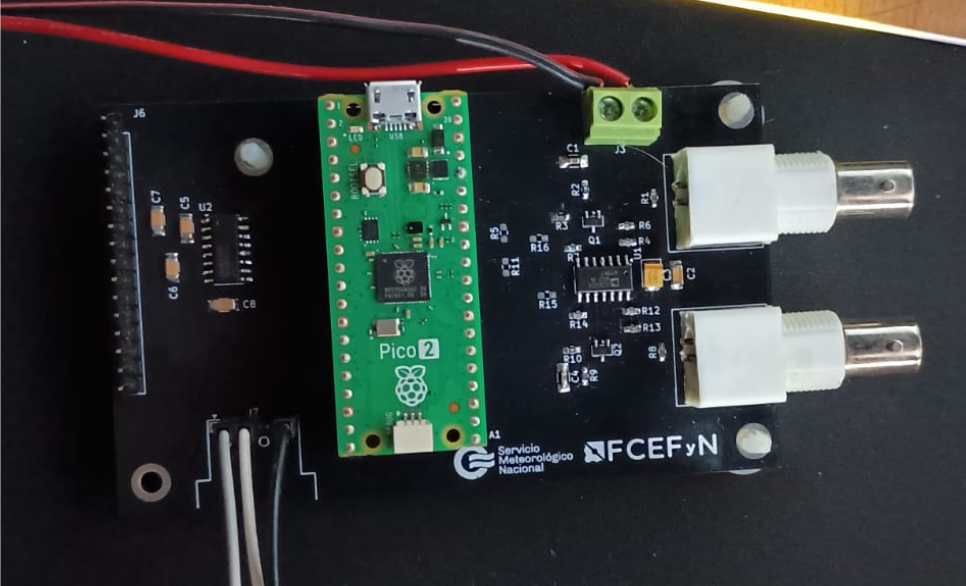
\includegraphics[width=0.7\textwidth]{figuras/9_prototipo.png}
      \caption{Placa de control ensamblada (Fuente: elaboración propia).}
      \label{fig:placaarmada}
\end{figure}

La placa de control reúne en una única pieza los dos canales de detección de picos correspondientes a las señales $P_+$ y $P_-$, el módulo Raspberry Pi Pico~2 montado sobre conectores hembra de $2\times20$ pines y el transceptor MAX3232 con su conector DB9. La alimentación ingresa por una bornera doble de $+12$~V y masa, y las entradas analógicas se materializan mediante conectores BNC ubicados sobre el borde contiguo a los amplificadores.

Para su emplazamiento definitivo, el conjunto se fijó sobre un panel de acrílico montado en el frente del equipo, de modo que los conectores de entrada, el enlace serie hacia el \emph{seeder} y el puerto USB hacia la computadora de control quedaran accesibles. Esta disposición concentra en un único plano frontal todos los puntos de conexión del lazo de sintonización: las salidas de los amplificadores de transimpedancia de los cuatro fotodetectores, las dos entradas para las señales $P_+$ y $P_-$ y el puerto USB.

\begin{figure}[htpb]
      \centering
      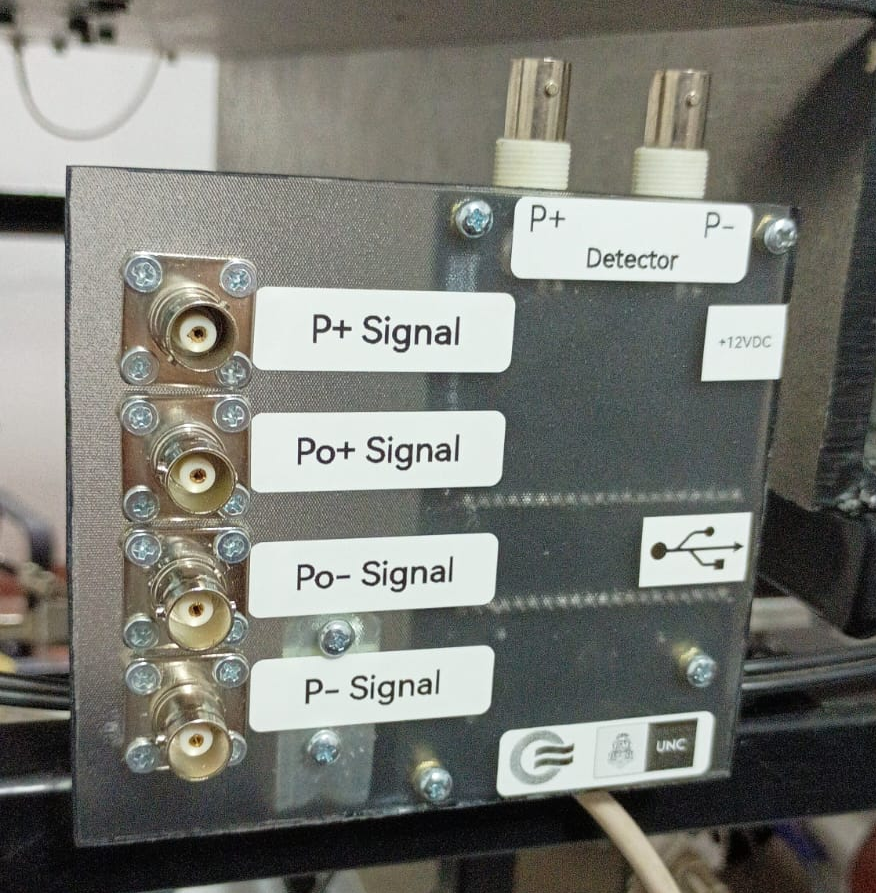
\includegraphics[width=0.7\textwidth]{figuras/9_panelacrilico.png}
      \caption{Panel de acrílico sobre el cual se encuentra montada la placa de control y bornes de salida del TIA (Fuente: elaboración propia).}
      \label{fig:panel}
\end{figure}

La señal de sincronismo del láser \emph{host} se toma del mismo y se adapta al rango lógico del microcontrolador mediante el divisor resistivo descrito en el Capítulo~\ref{cap:micro}. La comunicación con el láser \emph{seeder} se establece por el enlace RS-232 a través del conector DB9. Finalmente, el vínculo con la computadora de supervisión se realiza por USB, sobre el cual el \emph{firmware} expone una consola en modo CDC. Ninguna de estas interfaces exige modificar el camino óptico ni la electrónica de detección original del instrumento, lo que permite revertir la instalación y regresar a la configuración anterior sin intervención adicional.

\section{Funcionalidad del conjunto}
\label{sec:me-funcionalidad}

El sistema cumple, sobre el instrumento montado, las funciones que se enuncian a continuación.

\begin{itemize}
  \item El microcontrolador digitaliza el valor retenido por el detector de picos del canal que corresponda, alternando entre $P_+$ y $P_-$ en disparos consecutivos. El número de picos promediados por canal es configurable en caliente.
  \item El \emph{firmware} calcula el cociente entre ambos canales y corrige el punto de consigna de temperatura del calefactor del \emph{seeder} según la ley de control por histéresis con banda muerta multiplicativa descrita en la Sección~\ref{sec:fw-control}, manteniendo la longitud de onda del láser sobre la línea de absorción del iodo.
  \item Los modos de barrido en lazo abierto recorren el rango útil de temperatura mientras la interfaz registra los mínimos de cada canal, lo que permite localizar el punto de operación.
  \item La secuencia descrita en la Sección~\ref{sec:hmi-auto} encadena cuatro pasos individuales: la detención del barrido, la escritura del punto medio entre los mínimos, la espera de estabilización térmica y el cierre del lazo o sintonización, sin intervención directa del operador.
  \item El \emph{setpoint} se mantiene acotado al intervalo $[h_{\min}, h_{\max}]$ declarado en el \emph{firmware}; si el barrido lo excede, el controlador invierte el sentido y anula la sintonía del \emph{seeder}.
  \item La interfaz presenta el estado del enlace, el estado de las escrituras protegidas, la condición de \emph{second mode} del \emph{seeder} y las amplitudes medidas en función de la temperatura, visualizadas en la Figura~\ref{fig:tandem}, junto con la banda de alarmas jerarquizada de la Sección~\ref{sec:hmi-alarmas}, si es que existen alarmas activas.
  \item Cada sesión genera un archivo completo de operación y un archivo CSV con una fila por ciclo de control, según el contrato de columnas establecido en la Sección~\ref{sec:fw-log}.
\end{itemize}

\begin{figure}[htpb]
      \centering
      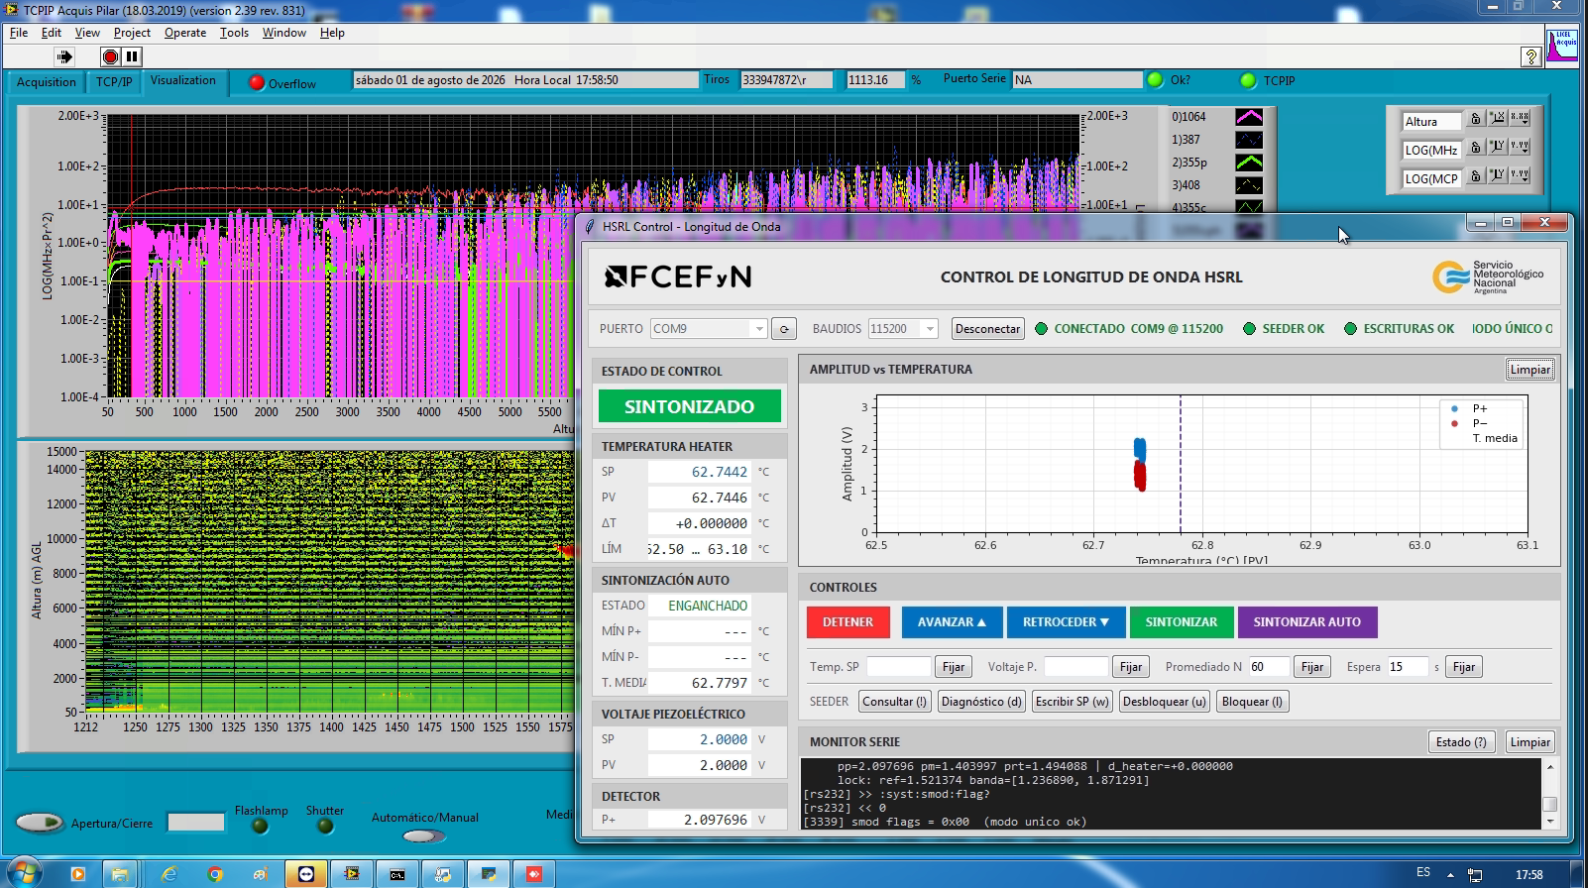
\includegraphics[width=0.7\textwidth]{figuras/9_tandem.png}
      \caption{Software de control de lidar (LABView) operando en conjunto con la HMI implementada (Fuente: elaboración propia).}
      \label{fig:tandem}
\end{figure}

Corresponde señalar que el lazo de control reside íntegramente en el microcontrolador. La interfaz de supervisión actúa como observador y como emisor de comandos, pero no forma parte del lazo: si la computadora se desconecta o el programa se cierra, el \emph{firmware} continúa sosteniendo la sintonización. Esta propiedad es la que habilita la operación desatendida planteada en la Sección~\ref{sec:formulacion_problema}.

\section{Instrucciones de operación}
\label{sec:me-manual}

\subsection{Organización de la pantalla}

La interfaz, cuyo aspecto se muestra en la Figura~\ref{fig:hmiopus}, distribuye el contenido en cuatro zonas siguiendo la jerarquía de pantallas descrita en la
Sección~\ref{sec:isa101}.

\begin{itemize}
      \item La \textbf{barra superior} concentra el establecimiento del enlace (selector
        \textbf{PUERTO}, selector \textbf{BAUDIOS} y botón \textbf{Conectar}) junto a
        los cuatro indicadores permanentes de estado: enlace USB, respuesta del
        \emph{seeder}, habilitación de las escrituras y condición de \emph{second mode}.
      \item La \textbf{columna izquierda} agrupa los valores del proceso en bloques:
        \textbf{ESTADO DE CONTROL}, que informa el modo vigente con un indicador de
        gran tamaño; \textbf{TEMPERATURA HEATER}, con el \emph{setpoint} (SP), la
        temperatura medida (PV), su diferencia ($\Delta T$) y el límite de seguridad
        alcanzado (LÍM); \textbf{SINTONIZACIÓN AUTO}, con los mínimos registrados de
        cada canal y la temperatura media resultante; \textbf{VOLTAJE
        PIEZOELÉCTRICO}; \textbf{DETECTOR}, con las amplitudes $P_+$, $P_-$ y su
        cociente; y \textbf{SINTONIZACIÓN}, con la referencia y la banda muerta
        vigentes.
      \item El \textbf{gráfico central} representa la amplitud de ambos canales en
        función de la temperatura, con una línea vertical que marca la temperatura
        media entre los mínimos. El botón \textbf{Limpiar} descarta los puntos
        acumulados.
       \item El \textbf{panel de control} reúne los cinco botones de modo, los campos de parámetro con su botón \textbf{Fijar} y la fila de comandos dirigidos al \emph{seeder}. Debajo, el \textbf{MONITOR SERIE} reproduce la terminal de la sesión y admite el envío de comandos sueltos.
\end{itemize}

La correspondencia entre cada control y la acción que ejecuta se resume en la
Tabla~\ref{tab:me-controles}. Entre paréntesis se indica el comando equivalente del
\emph{firmware} (Sección~\ref{sec:fw-consola}), de modo que toda operación puede
realizarse también desde el monitor serie si la interfaz no estuviera disponible.

\begin{table}[htpb]
\centering
  \begin{tabular}{@{}p{0.30\textwidth}p{0.62\textwidth}@{}}
  \toprule
  \textbf{Control} & \textbf{Acción} \\
  \midrule
  \multicolumn{2}{@{}l}{\textit{Modos de operación}} \\
  \textbf{DETENER} (\texttt{s})   & Interrumpe el barrido y la sintonización. Deja el \emph{setpoint} en su último valor. \\
  \textbf{AVANZAR} (\texttt{f})   & Barrido ascendente en lazo abierto, aplicando el paso grueso en cada ciclo. \\
  \textbf{RETROCEDER} (\texttt{b})& Barrido descendente en lazo abierto. \\
  \textbf{SINTONIZAR} (\texttt{g})& Cierra el lazo tomando como referencia el cociente de referencia de dos ciclos atrás. \\
  \textbf{SINTONIZAR AUTO}        & Ejecuta la secuencia completa de la Sección~\ref{sec:hmi-auto}: detiene, escribe la temperatura media, aguarda la estabilización y cierra el lazo. \\
  \midrule
  \multicolumn{2}{@{}l}{\textit{Parámetros (se confirman con \textbf{Fijar})}} \\
  \textbf{Temp. SP} (\texttt{T})      & \emph{Setpoint} del calefactor. \\
  \textbf{Voltaje P.} (\texttt{P})    & Tensión del piezoeléctrico del \emph{seeder}. \\
  \textbf{Promediado N} (\texttt{A})  & Cantidad de picos a promediar por canal. \\
  \textbf{Espera} (\texttt{E})        & Pausa de estabilización térmica al inicio de cada ciclo, en segundos. \\
  \midrule
  \multicolumn{2}{@{}l}{\textit{Comandos al \emph{seeder}}} \\
  \textbf{Consultar} (\texttt{!})     & Lee temperatura y tensión actuales del \emph{seeder}. \\
  \textbf{Diagnóstico} (\texttt{d})   & Consulta el estado de la protección y vacía la cola de errores. \\
  \textbf{Escribir SP} (\texttt{w})   & Fuerza la escritura inmediata del \emph{setpoint} y verifica su aceptación. \\
  \textbf{Desbloquear} (\texttt{u})   & Habilita los comandos protegidos. \\
  \textbf{Bloquear} (\texttt{l})      & Vuelve a proteger los comandos de escritura. \\
  \midrule
  \multicolumn{2}{@{}l}{\textit{Monitor serie}} \\
  \textbf{Estado} (\texttt{?})        & Solicita el envío completo de parámetros y la lista de columnas del registro. \\
  \textbf{Limpiar}                    & Vacía la consola en pantalla, sin afectar los archivos de registro. \\
  \bottomrule
  \end{tabular}
  \caption{Controles de la interfaz y comando equivalente del \emph{firmware} (Fuente: elaboración propia).}
  \label{tab:me-controles}
\end{table}

\subsection{Puesta en marcha}

El procedimiento de arranque es el siguiente:

\begin{enumerate}
  \item Verificar que los conectores BNC de $P_+$ y $P_-$, la entrada de sincronismo y el cable DB9 hacia el \emph{seeder} se encuentren firmemente asentados en el panel frontal.
  \item Verificar la energización de la placa con la fuente de $+12$~V. Cuando el LED se encuentra prendido fijamente el sistema está listo para operar.
  \item Conectar el cable USB a la computadora de supervisión y ejecutar la interfaz mediante el inicio de \texttt{hmi.py}.
  \item Seleccionar el puerto serie correspondiente e iniciar la comunicación mediante el botón \textbf{Conectar}. La barra superior debe indicar el enlace USB establecido, el \emph{seeder} respondiendo y las escrituras habilitadas.
\end{enumerate}

Si el indicador \textbf{ESCRITURAS} señala que los comandos permanecen protegidos,
debe pulsarse \textbf{Desbloquear} antes de intentar cualquier ajuste; en caso
contrario el \emph{seeder} descarta silenciosamente los \emph{setpoints} enviados.

\subsection{Localización del punto de operación}

Con el láser en régimen y el sistema recibiendo pulsos de sincronismo, se ordena un
barrido pulsando \textbf{AVANZAR} o \textbf{RETROCEDER}, según el sentido en que se
desee recorrer el rango de temperatura. El indicador \textbf{ESTADO DE CONTROL} pasa
a señalar el modo activo y el gráfico comienza a poblarse con las amplitudes de
$P_+$ y $P_-$ en función de la temperatura. A medida que avanza el barrido, los
campos \textbf{MÍN P+} y \textbf{MÍN P-} conservan el valor mínimo alcanzado por cada
canal junto con la temperatura a la que se produjo y \textbf{T. MEDIA} muestra el
punto medio resultante.

El barrido debe sostenerse hasta que ambos mínimos hayan quedado registrados,
condición que se verifica observando que las dos curvas del gráfico hayan atravesado
su valle y que \textbf{T. MEDIA} exhiba un valor estable. Si el punto de consigna
alcanza un extremo del rango de seguridad, el \emph{firmware} invierte el sentido del
barrido por sí solo.

\subsection{Sintonización}

Habiendo realizado múltiples barridos, se dispone de dos opciones de sintonización.

El procedimiento automático consiste en pulsar \textbf{SINTONIZAR AUTO}. La interfaz detiene el barrido,
escribe la temperatura media como punto de consigna, fuerza su escritura, aguarda la
estabilización térmica, deja transcurrir cuatro ciclos y recién entonces cierra el
lazo. El avance de la secuencia se sigue en el campo \textbf{ESTADO} del bloque
\textbf{SINTONIZACIÓN AUTO}. Si no hay mínimos registrados, o si la temperatura media
cae fuera del rango declarado por el \emph{firmware}, la secuencia no se inicia y el
motivo aparece en el monitor serie.

El procedimiento manual reproduce los mismos pasos uno a uno: pulsar
\textbf{DETENER}; ingresar la temperatura media en \textbf{Temp. SP} y confirmarla
con \textbf{Fijar}; pulsar \textbf{Escribir SP} para forzar la escritura sin esperar
a que concluya el ciclo en curso; esperar a que \textbf{PV} coincida con el valor de
\textbf{SP} en el bloque \textbf{TEMPERATURA HEATER}; y finalmente pulsar
\textbf{SINTONIZAR}. Conviene esta vía cuando se desea fijar un punto de trabajo
distinto del punto medio, por ejemplo para comprobar el correcto desplazamiento de las líneas de absorción o el camino óptico de los haces.

En ambos casos, el cierre correcto del lazo se reconoce porque \textbf{ESTADO DE
CONTROL} indica el modo de sintonización.

\subsection{Operación en régimen}

Una vez sintonizado el sistema, la operación no requiere intervención. El operador dispone de los siguientes elementos para evaluar el estado del sistema:

\begin{itemize}
  \item La ausencia de la banda de alarmas, que sólo se despliega ante una
        condición activa.
  \item La permanencia del \emph{setpoint} dentro del rango de seguridad, visible
        sobre el eje de abscisas del gráfico y en el campo \textbf{LÍM}.
  \item El indicador \textbf{MODO ÚNICO} de la barra superior, que advierte cuando el
        \emph{seeder} abandona la operación monomodo y las mediciones del ciclo dejan
        de ser representativas.
  \item El campo \textbf{CICLO}, cuyo incremento regular confirma que el
        \emph{firmware} sigue recibiendo pulsos de sincronismo.
\end{itemize}

Ante la indicación de segundo modo, la acción correctiva consiste en ingresar un
nuevo valor en \textbf{Voltaje P.} y confirmarlo con \textbf{Fijar}, hasta restituir
la operación monomodo. El \emph{firmware} informa la condición pero no actúa sobre
ella de manera deliberada, de modo que la decisión queda en el operador.

\subsection{Archivos generados}

Cada ejecución de la interfaz produce dos archivos en la carpeta \texttt{logs/}, nombrados con la misma marca temporal de inicio del HMI: un archivo de texto con la totalidad de los comandos enviados y las líneas recibidas, destinada al análisis de incidentes, y un archivo CSV con una fila por ciclo de control, destinado al análisis de los datos. El encabezado del CSV se construye a partir de los nombres de columna que el propio \emph{firmware} declara, según lo detallado en la Sección~\ref{sec:hmi-registro}.

\subsection{Detención}

Para detener el control se pulsa \textbf{DETENER}, que interrumpe tanto el barrido
como la sintonización y deja el punto de consigna en su último valor. El indicador
\textbf{ESTADO DE CONTROL} pasa a señalar la condición de detenido. Este botón
cancela además cualquier secuencia de sintonización automática en curso, por lo que
opera como parada de emergencia del lazo.

El \emph{seeder} conserva el último \emph{setpoint} aun cuando la placa se
desenergice, de modo que un rearranque posterior parte de una condición conocida. Si
se desea impedir escrituras accidentales antes de retirar el equipo de servicio,
conviene pulsar \textbf{Bloquear} para volver a proteger los comandos de escritura.

\section{Ensayos sobre el sistema HSRL del Observatorio de Pilar}
\label{sec:me-ensayos}

El conjunto se instaló sobre el sistema HSRL del Observatorio Geofísico y Meteorológico de Pilar y se sometió a una serie de ensayos
orientados a verificar su desempeño en condiciones reales de operación.

\subsection{Verificación funcional inicial}

El primer ensayo tuvo por objeto comprobar que el sistema fuera capaz de cambiar el punto de operación y sostenerlo con el instrumento en funcionamiento. Primero se mantuvo fija una temperatura, para determinar el comportamiento del sistema en estado estacionario. El resultado se muestra en la Figura~\ref{fig:stop}, donde se observa que el lazo mantiene la temperatura de consigna en lazo abierto durante un período de 13 horas, sin intervención del operador. Cabe destacar la variación de amplitud en los canales $P_+$ y $P_-$, que se debe a la fluctuación de temperatura en la celda de iodo, puesto que la misma posee un control ON/OFF. Debido a que la temperatura de la celda es proporcional a su absorción, la variación de amplitud en los canales es esperable y no afecta el desempeño del lazo de control.

\begin{figure}[htpb]
      \centering
      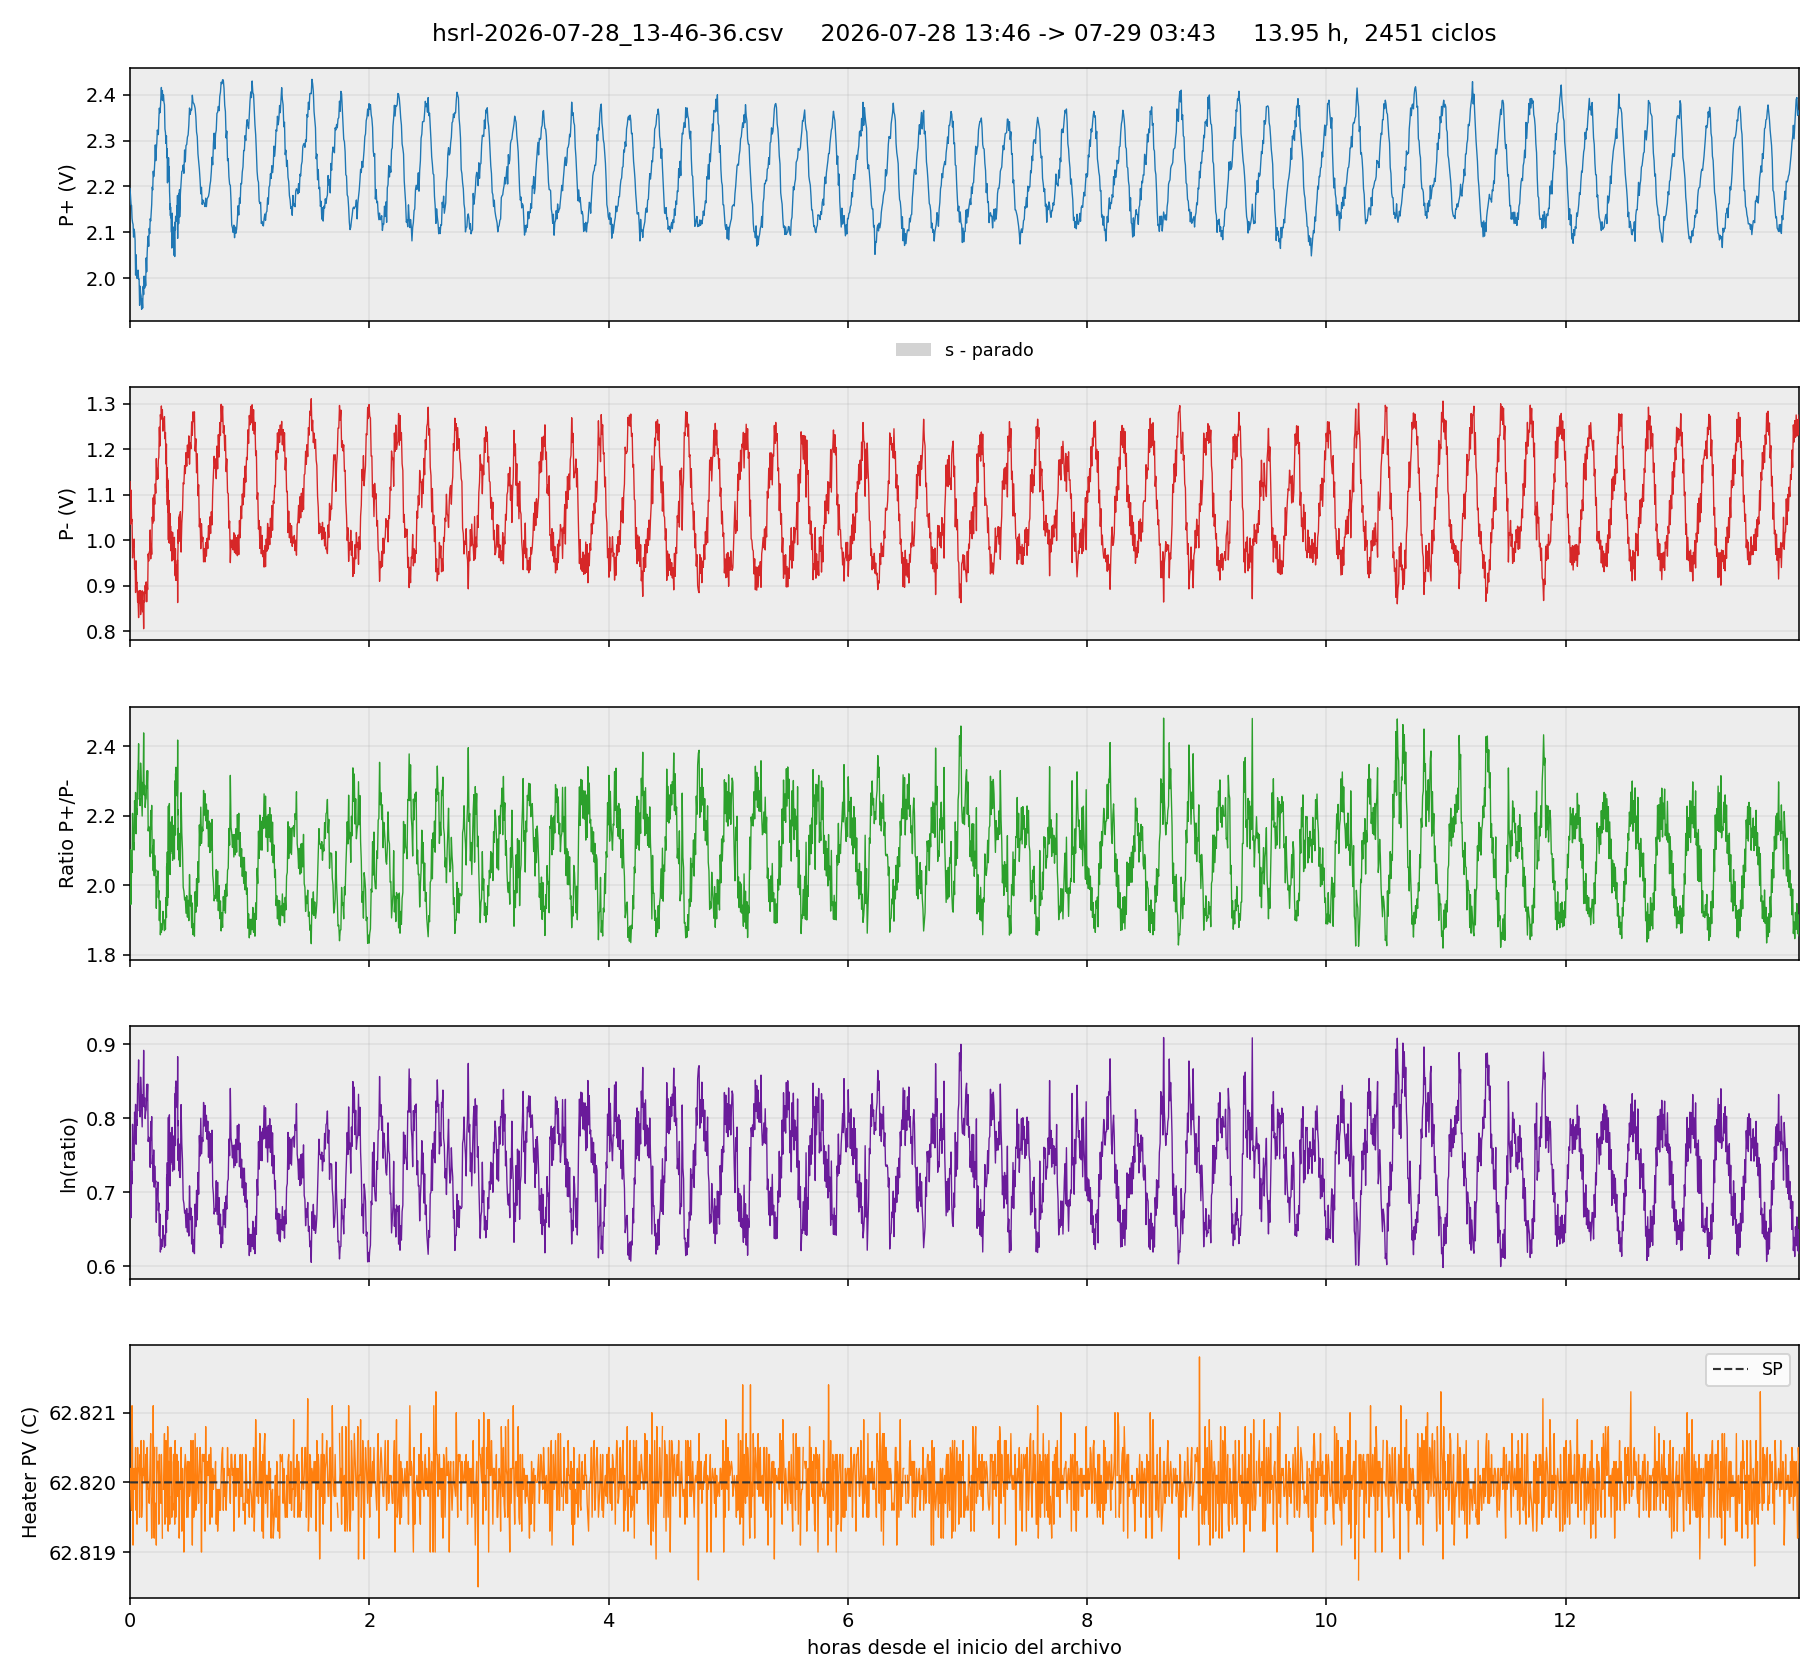
\includegraphics[width=1\textwidth]{figuras/9_stop.png}
      \caption{CSV generado por la HMI, luego de mantener fija una temperatura de 62,82\,\textcelsius\ durante 13 horas (Fuente: elaboración propia).}
      \label{fig:stop}
\end{figure}

Luego de verificar la correcta operación para selección de temperatura a lazo abierto, se iniciaron sucesivos barridos de temperatura, ilustrados en la Figura~\ref{fig:sweep}. En cada barrido se registraron los mínimos de cada canal y se determinó el punto medio entre ambos, que constituye el punto de trabajo para el cierre del lazo. La Figura~\ref{fig:sweep} muestra un barrido de temperatura de 62,3\,\textcelsius\ a 63,1\,\textcelsius, donde se observa la variación de las señales $P_+$ y $P_-$ con la temperatura.

\begin{figure}[htpb]
      \centering
      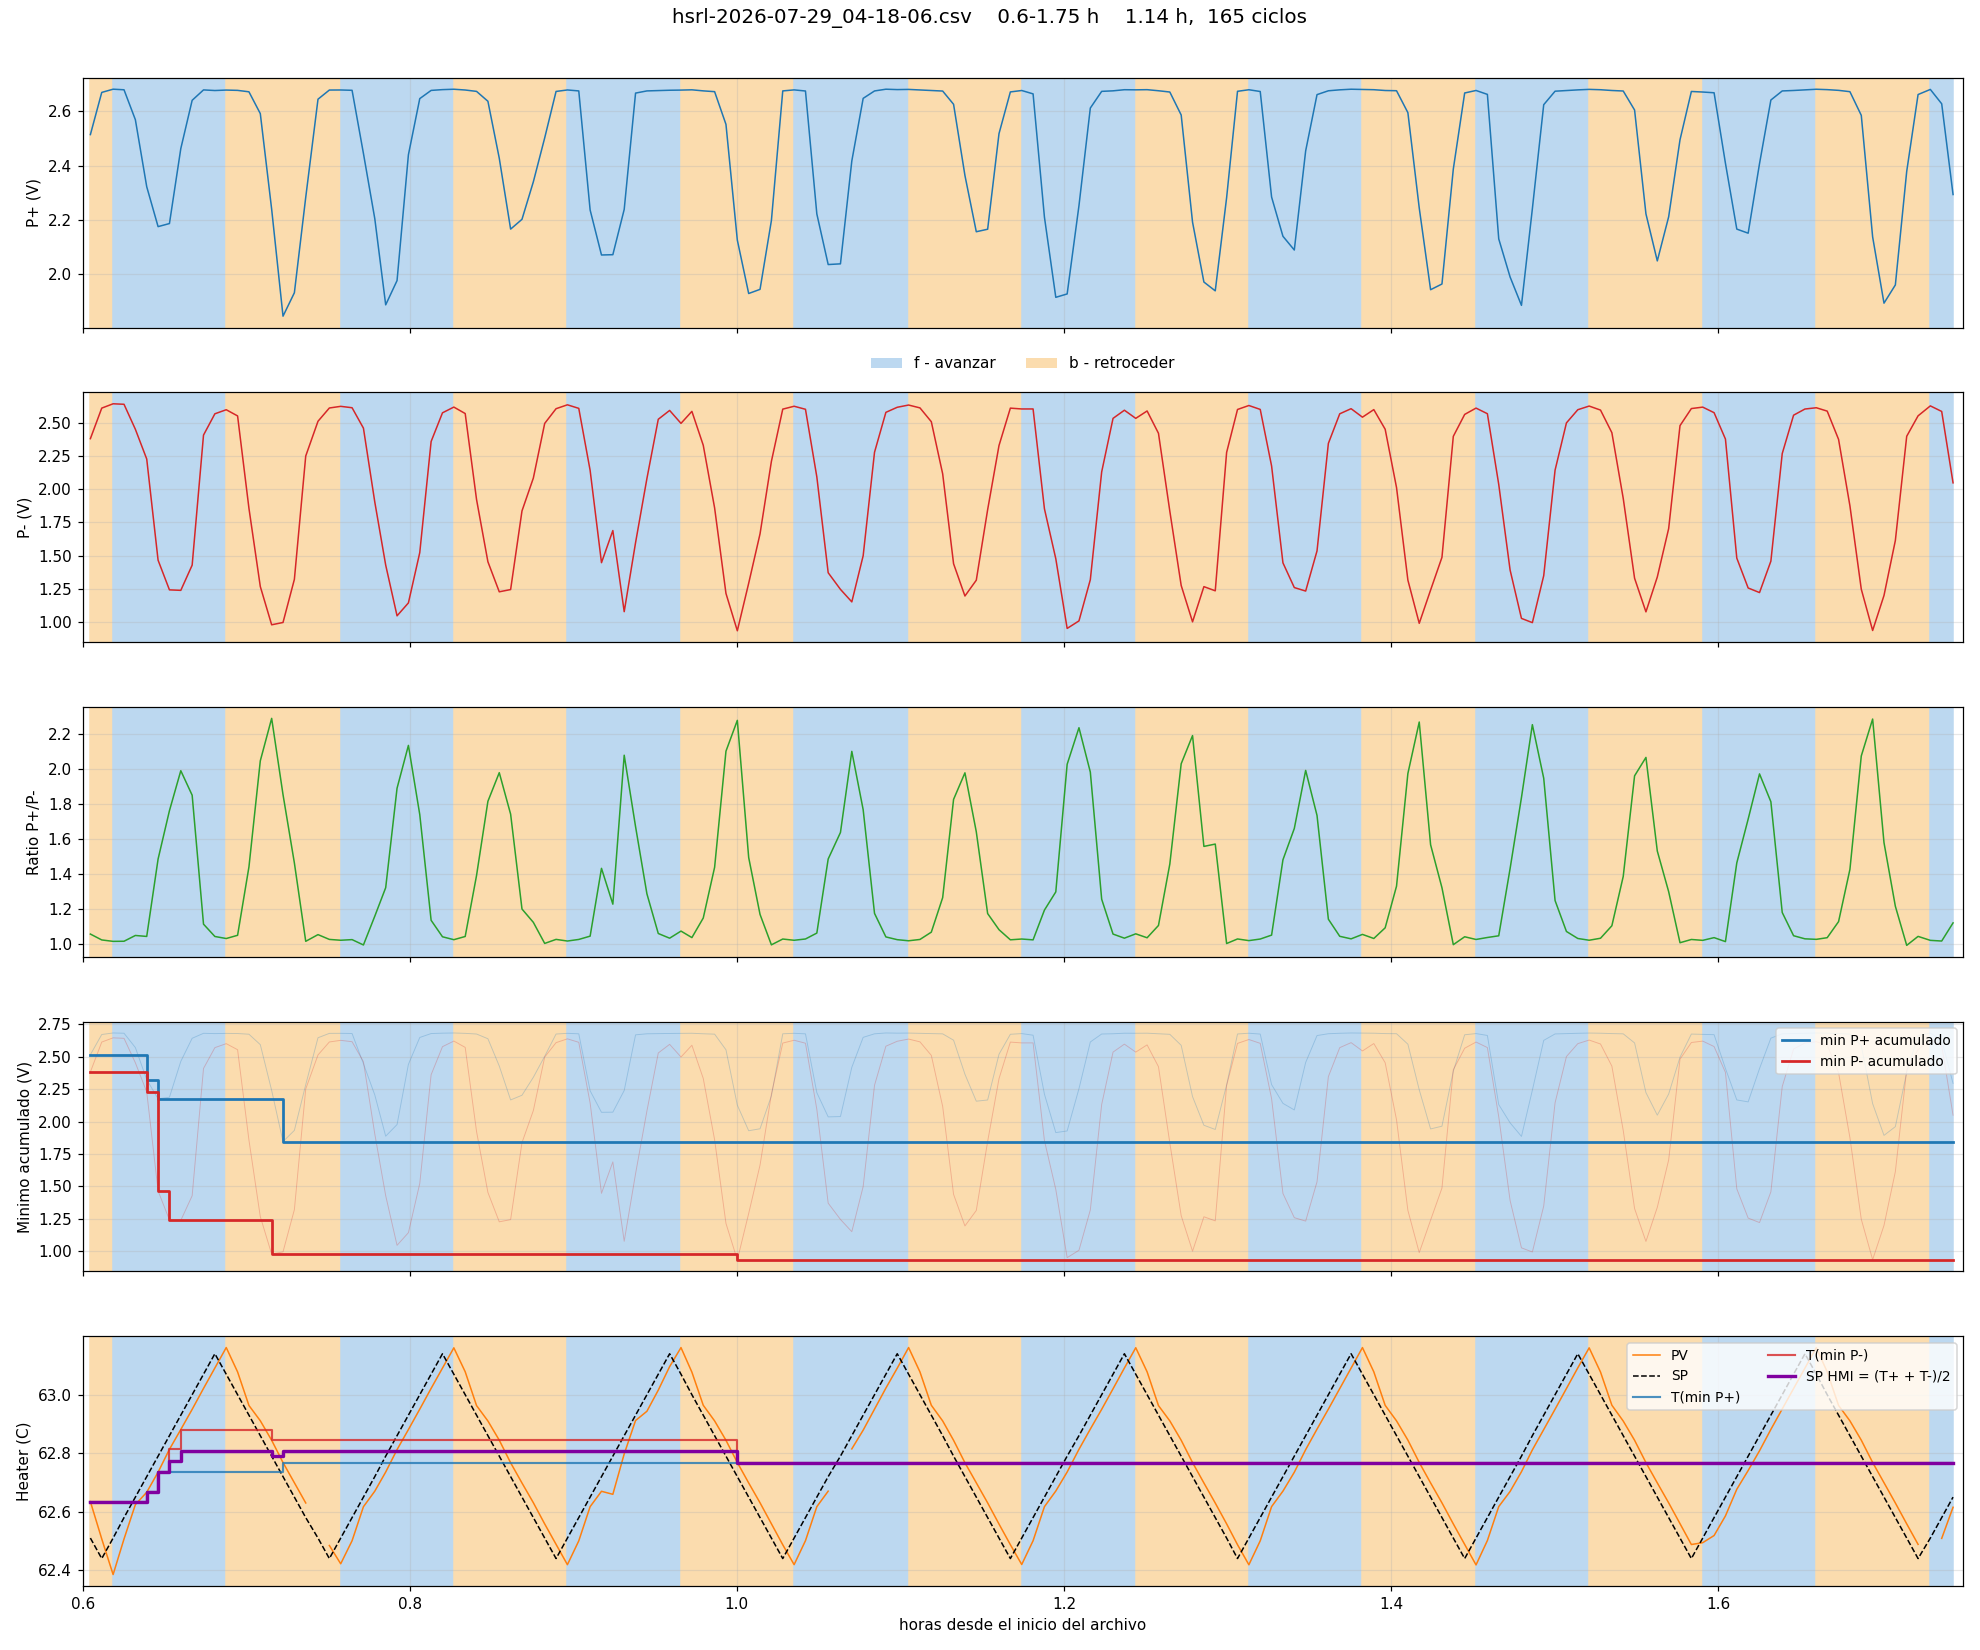
\includegraphics[width=1\textwidth]{figuras/9_sweeps.png}
      \caption{Barridos en temperatura para encontrar punto de operación. El punto de operación aparece luego de 2 horas de barridos (Fuente: elaboración propia).}
      \label{fig:sweep}
\end{figure}

\subsection{Ensayos de estabilidad}

Se realizaron una serie de mediciones de corto plazo para verificar la estabilidad del sistema. Primero se utilizó el instrumento en operación continua, esto es, con el láser disparando a su frecuencia total de $10$~Hz. Las condiciones atmosféricas variaron desde un día despejado hacia un día parcialmente nublado. Para el análisis de la señal lidar se utilizó el código Python almacenado en el repositorio \emph{quicklook} \cite{quicklook}.

La correcta sintonización del instrumento en modo automático se puede visualizar en la Figura~\ref{fig:sintonia}. Para la sintonización, se comandó al equipo a realizar barridos durante un período de 2 horas. Luego de 2 horas, se accionó el comando automático de la HMI. La HMI colocó el punto de trabajo en 62,78\,\textcelsius, definiendo una relación determinada entre $P_+$ y $P_-$. El controlador mediante ajustes finos llevó la temperatura del \emph{seeder} a 62,72\,\textcelsius\ manteniendo la relación entre $P_+$ y $P_-$, \texttt{coe} en el valor definido por la temperatura. 

\begin{figure}[htpb]
      \centering
      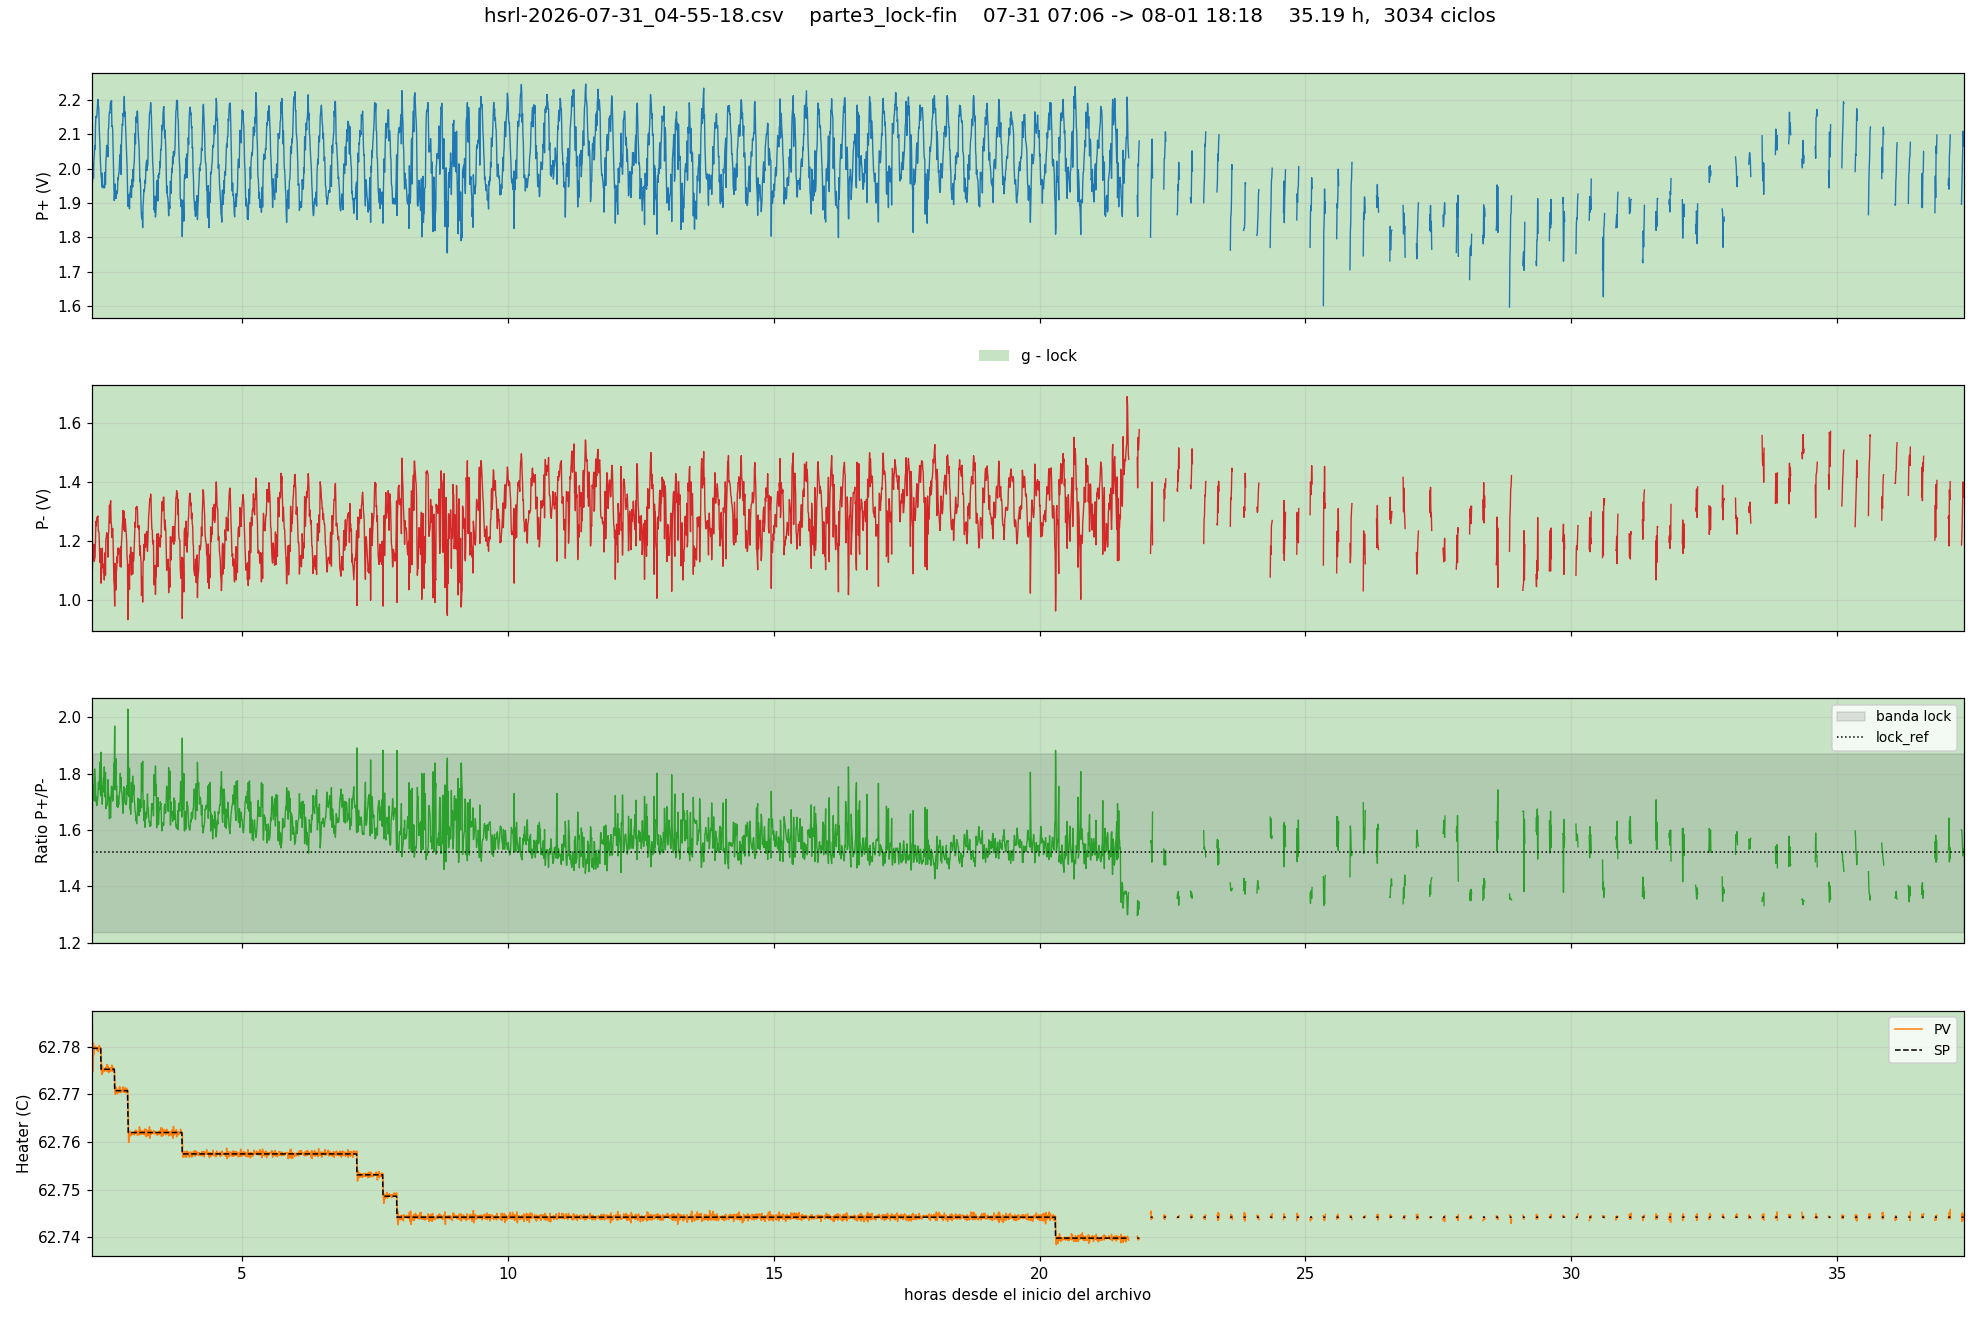
\includegraphics[width=1\textwidth]{figuras/9_sintonía.png}
      \caption{Sintonización del sistema en modo automático (Fuente: elaboración propia).}
      \label{fig:sintonia}
\end{figure}


\begin{figure}[htpb]
      \centering
      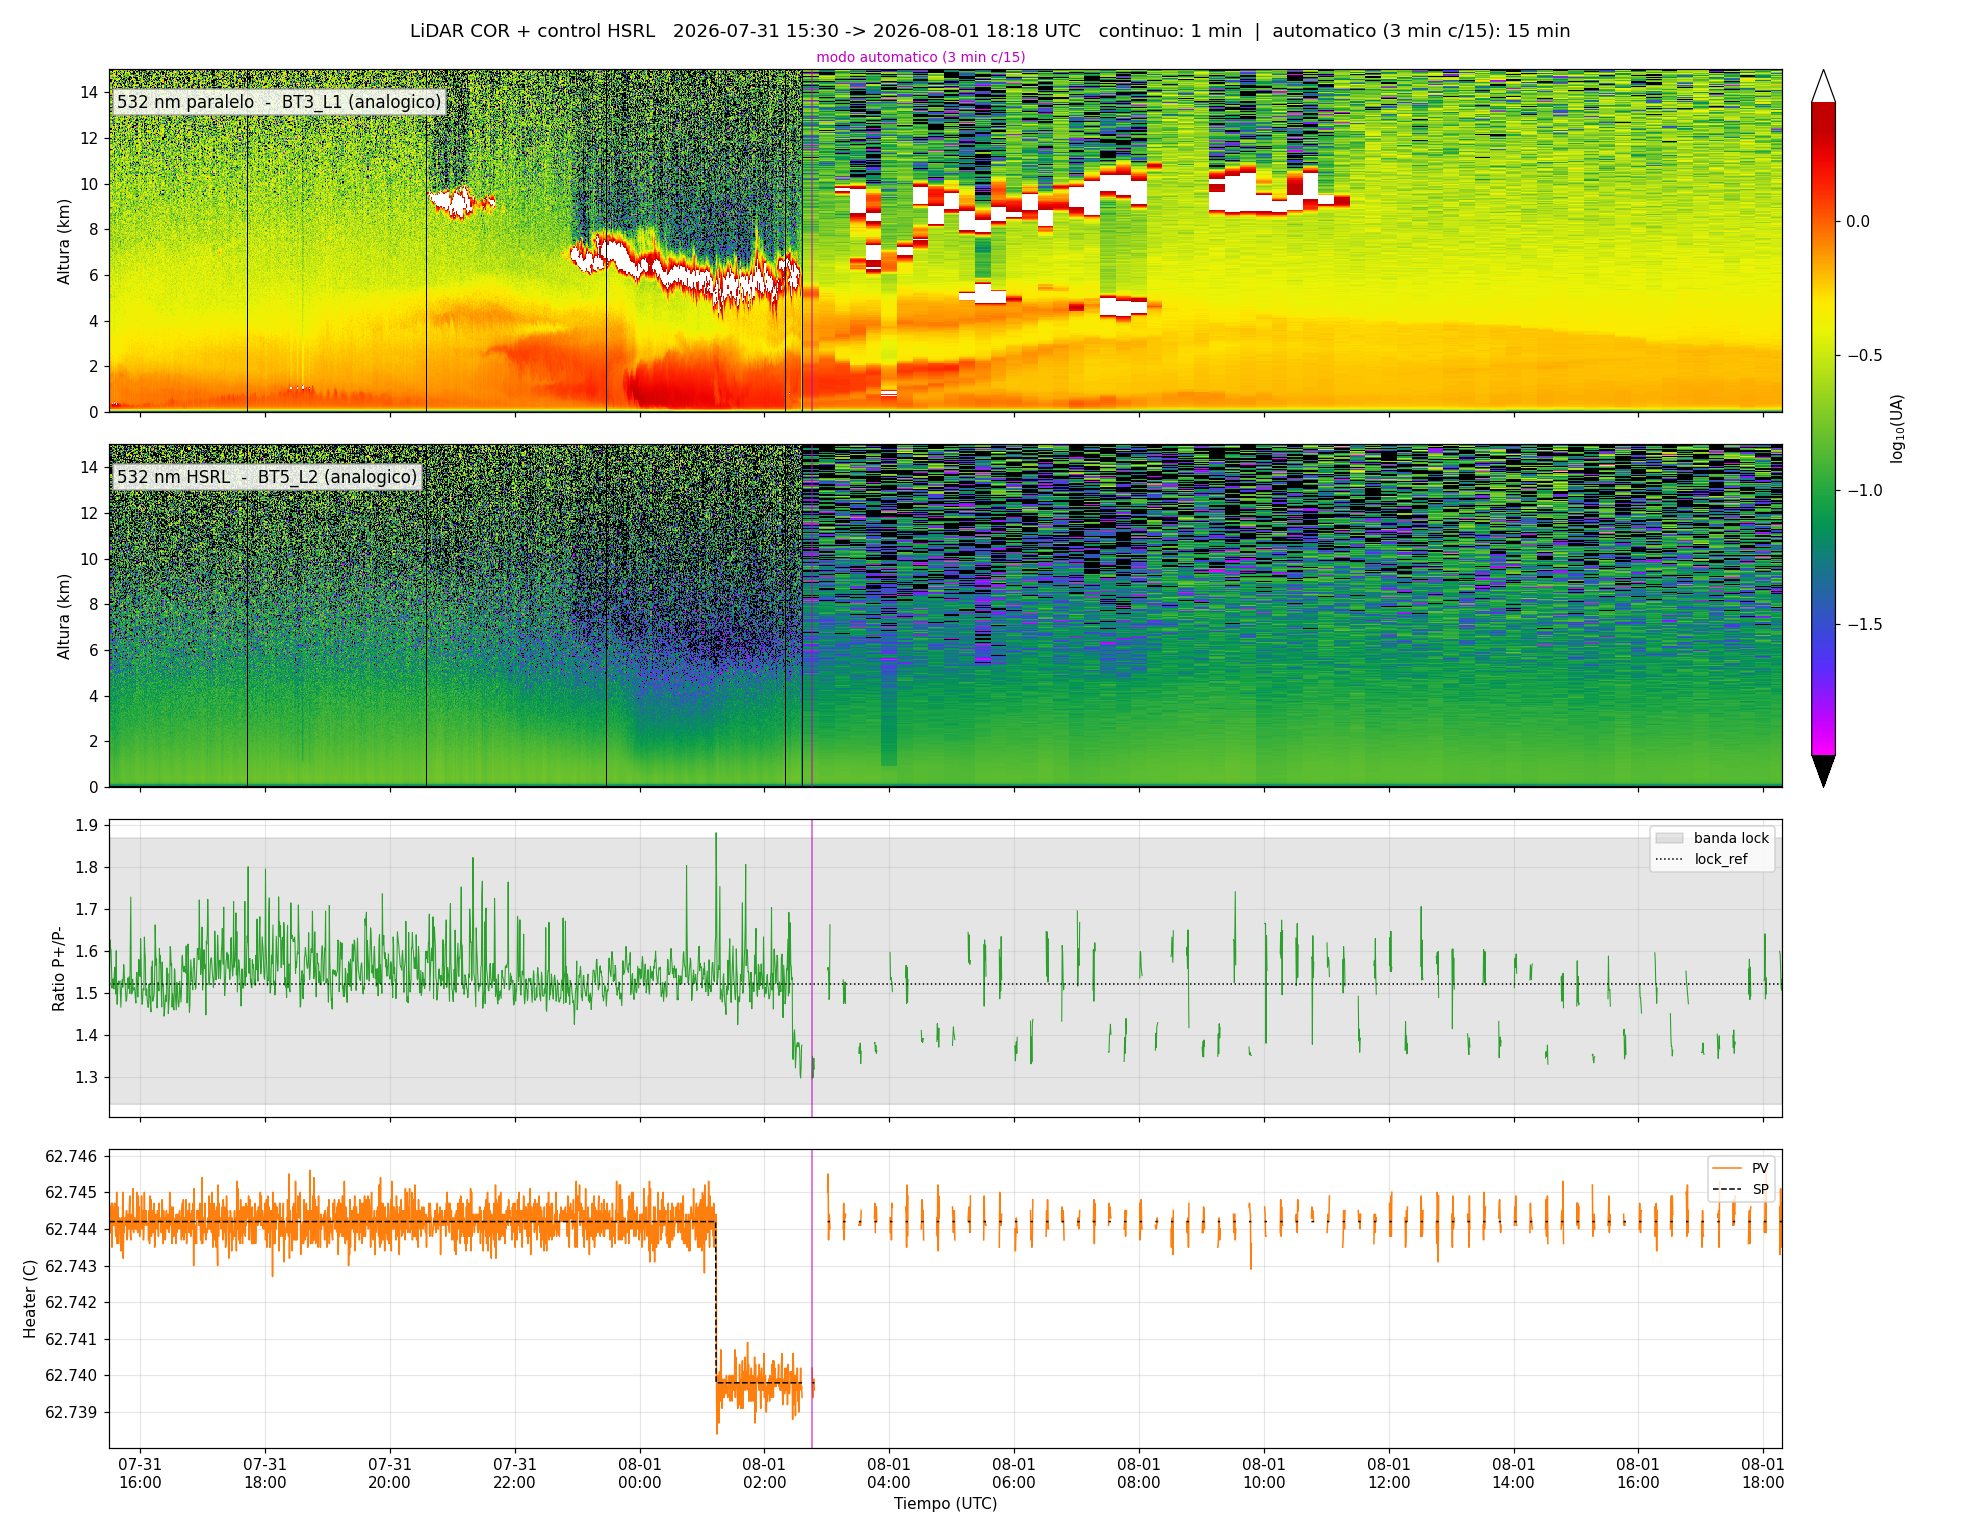
\includegraphics[width=1\textwidth]{figuras/9_autocontinuo.png}
      \caption{Mediciones de atmósfera en canal elástico 532~nm y canal HSR (Fuente: elaboración propia).}
      \label{fig:autocontinuo}
\end{figure}

Luego de tener el sistema sintonizado, se realizaron mediciones de la atmósfera. En la Figura~\ref{fig:autocontinuo} el diagrama de color superior muestra la señal del canal elástico a 532~nm, mientras que el diagrama de color inferior muestra la señal del canal HSR. La diferencia principal entre ambos canales radica en la sensibilidad a la señal retrodispersada por aerosoles. 

Se observan dos evidencias principales que permiten inferir el correcto funcionamiento del canal HSR. La primera es que, ante una fuerte presencia de aerosoles en el rango de 0 a 4 km, el canal HSR muestra una señal mucho más débil que el canal elástico, lo cual es consistente con la teoría de retrodispersión (ya que el canal HSR filtra la componente de los aerosoles). La segunda es que la señal retrodispersada por moléculas a mayor altitud (6 a 10 km) disminuye; esto se debe a la atenuación (extinción) que sufre el haz de luz al atravesar la capa de aerosoles ubicada en los niveles inferiores.

A partir de las 3:00 AM (UTC) el día 01/08/2026, el modo de operación del láser cambia a automático. En este modo, diseñado para preservar la vida útil de la lámpara del láser, el mismo dispara durante 3 minutos cada 15 minutos. Esto se observa en la Figura~\ref{fig:autocontinuo} como franjas horizontales de señal de menor resolución. A pesar de este cambio, el canal HSR sigue mostrando un comportamiento consistente con la teoría de retrodispersión, lo que indica que el lazo de control mantiene la sintonización del láser en la línea de absorción del iodo.

En los últimos dos gráficos de la Figura~\ref{fig:autocontinuo} se observa cómo se mantiene la sintonización del instrumento, realizando un único cambio el día 01/08/2026 a las 2:00 AM (UTC). Esto indica que el lazo de control mantiene la sintonización del láser en la línea de absorción del iodo, incluso cuando el modo de operación del láser cambia a automático. Si bien este análisis se realizó con mediciones cortas, es suficiente para mostrar la correcta sintonización del lazo en modo automático.

\section{Limitaciones conocidas del prototipo}
\label{sec:me-limitaciones}

El modelo descrito constituye un primer prototipo funcional y, como tal, conserva las limitaciones que se detallan a continuación. Su enunciado explícito busca delimitar el alcance de lo validado y orientar una eventual continuidad del trabajo.

\begin{itemize}
  \item El conversor del microcontrolador dispone de canales adicionales y el sistema óptico entrega las señales $P_0$, cuya digitalización podría aportar información al control. El prototipo no las incorpora.
  \item Ante la detección de operación \emph{second mode} el sistema informa la condición pero no descarta la medición ni suspende el lazo, de modo que la corrección queda a cargo del operador.
  \item Para simplificar el primer prototipo no se discriminó entre masa analógica y masa digital. Una revisión posterior de la placa debería evaluar el impacto de esta decisión sobre el piso de ruido de la etapa de detección.
  \item El prototipo no incorpora reguladores de tensión propios, indicadores luminosos ni pulsadores, por lo que depende de la fuente externa y del LED del módulo de desarrollo para la señalización de estado.
  \item Al controlar la temperatura de la celda de iodo mediante un lazo de histéresis, el sistema no puede garantizar una atenuación constante para una determinada temperatura de cavidad de \emph{seeder}. Debido a esto, la banda muerta multiplicativa es del orden del 20\%. Un control más preciso de la temperatura de la celda de iodo permitiría reducir la banda muerta y mejorar la estabilidad del lazo de control.

\end{itemize}

\part{Resultados y Conclusiones}
% =============================================================
% Resultados
% Apartado individual, no es un Capitulo
% =============================================================
\chapter*{Resultados}
\label{cap:resultados}
\phantomsection
\addcontentsline{toc}{chapter}{Resultados}

A la fecha de redacci\'on de este informe, los resultados obtenidos son
parciales, dado que el proyecto se encuentra en curso (ver
Secci\'on~\ref{sec:metodologia_intro}). Se resumen a continuaci\'on los
resultados alcanzados hasta el momento:

\begin{itemize}
  \item El circuito detector de picos dise\~nado (Cap\'itulo~\ref{cap:diseno_deteccion_picos})
        fue simulado y validado experimentalmente, confirmando su
        comportamiento lineal para tensiones de entrada superiores a
        0.8~V y su correcta respuesta ante pulsos de 100~ns
        \cite{informeEneFeb2026,informeAbril2026}.
  \item Las oscilaciones observadas en el prototipo inicial, atribuidas
        a capacidades par\'asitas, fueron resueltas mediante el
        rediseño de la placa con t\'ecnicas de ruteo para se\~nales de
        alta velocidad (Secci\'on~\ref{sec:mitigacion_parasitos})
        \cite{informeMarzo2026,informeAbril2026}.
  \item Se verific\'o la correcta comunicaci\'on entre la placa de
        control y el l\'aser seeder mediante el enlace RS232/MAX3232
        \cite{informeAbril2026}.
  \item Se implement\'o un primer borrador del software HMI, con
        comunicaci\'on funcional en sentido placa-PC
        \cite{informeAbril2026}.
  \item Avances parciales del proyecto fueron presentados en el ILRC32
        \cite{galvagno2026ilrc}.
\end{itemize}

PLACEHOLDER: completar este apartado con los resultados de la
validaci\'on integral del sistema (firmware completo, comunicaci\'on
bidireccional del HMI y mediciones sobre el canal HSR real), en
relaci\'on con los objetivos espec\'ificos planteados en la
Secci\'on~\ref{sec:objetivos_especificos}, una vez finalizada la etapa
de desarrollo restante.

% =============================================================
% Conclusiones
% Apartado individual, no es un Capitulo
% Sugerido: resultados vs SAT, conclusion general, aporte a la ingenieria
% =============================================================
\chapter*{Conclusiones}
\label{cap:conclusiones}
\phantomsection
\addcontentsline{toc}{chapter}{Conclusiones}

\section*{Resultados obtenidos en relaci\'on a la Solicitud de Aprobaci\'on de Tema}

De los ocho objetivos espec\'ificos planteados en la Solicitud de
Aprobaci\'on de Tema (Secci\'on~\ref{sec:objetivos_especificos}), el
dise\~no, la implementaci\'on y la validaci\'on del circuito de
detecci\'on (primer y segundo objetivos) se encuentran completos
\cite{informeEneFeb2026,informeAbril2026}. La selecci\'on del conjunto
ADC/microcontrolador (tercer objetivo) tambi\'en se encuentra completa
\cite{informeEneFeb2026}.

PLACEHOLDER: completar esta secci\'on con el estado final de los
objetivos restantes (programaci\'on del microcontrolador, comunicaci\'on
con el seeder, software de decisi\'on, HMI en Python y validaci\'on con
mediciones del sistema LiDAR) una vez finalizado el proyecto.

\section*{Conclusi\'on general}

PLACEHOLDER: redactar la conclusi\'on general del trabajo una vez
finalizada la etapa de integraci\'on y validaci\'on descrita en el
Cap\'itulo~\ref{cap:modelo_experimental}.

\section*{Aporte a la ingenier\'ia}

PLACEHOLDER: como se se\~nala en la Secci\'on~\ref{sec:antecedentes}, no
se registran antecedentes de proyectos integradores de la FCEFyN
vinculados al desarrollo de sistemas de control para lazos de alta
resoluci\'on espectral de instrumentos LiDAR \cite{sat2026}; esta
secci\'on debe completarse explicitando el aporte concreto del sistema
desarrollado a este campo una vez finalizado el proyecto.


% -------------------------------------------------------------
% BIBLIOGRAFIA Y REFERENCIAS (numeracion continua)
% -------------------------------------------------------------
% El titulo se compone con \chapter*, igual que Resultados y Conclusiones, para
% que herede el formato definido con titlesec. Por eso ambos \printbibliography
% van con heading=none: la opcion title no tiene efecto en ese caso.
\cleardoublepage
\chapter*{Bibliografía}
\phantomsection
\addcontentsline{toc}{chapter}{Bibliografía}
\printbibliography[type=book,heading=none]

\cleardoublepage
\chapter*{Referencias}
\phantomsection
\addcontentsline{toc}{chapter}{Referencias}
\printbibliography[nottype=book,heading=none]

% -------------------------------------------------------------
% ANEXOS
% -------------------------------------------------------------
\appendix

% Los anexos se numeran en romanos y se rotulan "Anexo" (no "Capitulo"),
% segun el manual de estilo. \appendix asigna letras por defecto.
\renewcommand{\thechapter}{\Roman{chapter}}
\titleformat{\chapter}[block]
  {\normalfont\bfseries\fontsize{14}{17}\selectfont}
  {Anexo \thechapter}{1em}{}

% En el indice, la entrada de capitulo se compone con \numberline{\thechapter},
% que para los anexos produce solo "I", "II", etc. Se redefine \numberline
% dentro del propio archivo .toc a partir de este punto, de modo que las
% entradas restantes queden rotuladas como "Anexo I: Titulo".
\renewcommand{\appendixname}{Anexo}
\addtocontents{toc}{\protect\let\protect\numberline\protect\anexonumberline}

% Orden segun aparicion en el cuerpo del informe.
% =============================================================
% Anexo I - Hojas de datos de componentes
% =============================================================
\chapter{Código fuente original del sistema HSR}
\label{anexo:hsrlnies}

El código realizado originalmente para el control HSRL, concentrado en el archivo \textbf{wvcnt\_lec.cpp} se encuentra en el repositorio de GitHub \cite{repo}.
\chapter{Esquemático de la placa de control}
\label{anexo:esquematico}

Se reproducen a continuación las láminas del esquemático de la placa de
control descripta en el Capítulo \ref{cap:placacontrol}, exportadas desde
el proyecto de KiCad. La primera corresponde a la hoja raíz y las
restantes a las hojas jerárquicas del circuito de detección y del
circuito digital. Las láminas se imprimen en orientación apaisada para
conservar la legibilidad de las referencias y de los valores de los
componentes.

\begin{hojaapaisada}
\includepdf[pages=-,scale=0.92,pagecommand={\pagestyle{fancy}}]%
  {anexos/pdf/esquematico.pdf}
\end{hojaapaisada}

\chapter{Circuito impreso (PCB) de la placa de control}
\label{anexo:pcb}

Se reproducen a continuación las láminas del circuito impreso descripto
en el Capítulo~\ref{cap:placacontrol}, exportadas desde el proyecto de
KiCad. Las primeras muestran por separado las capas de cobre y la
serigrafía; la última superpone todas las capas junto con el contorno de
placa y los componentes, tal como se envió a fabricación. Las láminas se
imprimen en orientación apaisada para conservar la escala del dibujo.

\begin{hojaapaisada}
\includepdf[pages=-,scale=0.92,pagecommand={\pagestyle{fancy}}]%
  {anexos/pdf/placa.pdf}
\includepdf[pages=-,scale=0.92,pagecommand={\pagestyle{fancy}}]%
  {anexos/pdf/placacompleta.pdf}
\end{hojaapaisada}

% =============================================================
% Anexo I - Hojas de datos de componentes
% =============================================================
\chapter{Hojas de datos de componentes}
\label{anexo:hojas_datos}

Las hojas de datos de los componentes utilizados en el desarrollo de la placa para control del HSRL se encuentran en el repositorio de GitHub \url{https://github.com/FGalvagno/hsrl-control-pi}. \cite{repo}

% =============================================================
% Anexo III - Codigo fuente relevante
% Lineas de codigo que no se incluyen en el cuerpo del informe.
% Si el codigo es extenso, referenciar el repositorio del proyecto.
% =============================================================
\chapter{C\'odigo fuente relevante}
\label{anexo:codigo}

El código fuente relevante para el control del HSRL se encuentra en el repositorio de GitHub \url{https://github.com/FGalvagno/hsrl-control-pi}. \cite{repo}
% =============================================================
% Anexo IV - Abstract presentado en el ILRC32
% Avances presentados en la 32.a International Laser Radar Conference
% (5-10 de julio de 2026) \cite{galvagno2026ilrc}.
% =============================================================
\chapter{Abstract presentado en el ILRC32}
\label{anexo:ilrc32}

En el presente anexo se incluye el abstract/p\'oster ``Advances on
Automation of Wavelength Tuning for High Spectral Resolution Lidar''
\cite{galvagno2026ilrc}, presentado por el autor junto a los directores
y colaboradores del proyecto en la 32.\textsuperscript{a} International
Laser Radar Conference (ILRC32), donde se resumieron los avances
alcanzados hasta ese momento en el circuito de detecci\'on de picos y en
el modelo del fotodiodo (ver Cap\'itulos~\ref{cap:fotodeteccion} y
\ref{cap:diseno_deteccion_picos}).

\includepdf[pages=1,scale=0.85,offset=0 -28pt,pagecommand={\pagestyle{fancy}}]{anexos/pdf/ILRC32_abstract.pdf}
\includepdf[pages=2-,scale=0.90,offset=0 10pt,pagecommand={\pagestyle{fancy}}]{anexos/pdf/ILRC32_abstract.pdf}
\includepdf[pages=-,scale=0.90,offset=0 10pt,pagecommand={\pagestyle{fancy}}]{anexos/pdf/ILRC32Poster.pdf}

% -------------------------------------------------------------
% ANEXO DE LA CATEDRA PI 
% -------------------------------------------------------------
\backmatter
\cleardoublepage
\phantomsection
\addcontentsline{toc}{chapter}{Anexo del Proyecto Integrador}
\chapter*{Anexo del Proyecto Integrador}
  En el presente anexo se incluyen la Solicitud de Aprobación de Tema y los informes mensuales de avance del proyecto, presentados a la Cátedra de Proyecto Integrador durante el desarrollo del mismo.
% =============================================================
% Solicitud de Aprobacion de Tema (SAT)
% IMPORTANTE: retirar datos personales y firmas del Director,
% Co-Director/es y Estudiante antes de incluir en el Informe Final.
% =============================================================
\section*{Solicitud de Aprobaci\'on de Tema}
\label{sec:anexo_sat}
\addcontentsline{toc}{section}{Solicitud de Aprobaci\'on de Tema}
\includepdf[pages=-]{anexos/pdf/SAT.pdf}
% =============================================================
% Informes Mensuales de Avance
% Ordenados por fecha. IMPORTANTE: retirar todo dato personal y firmas.
% =============================================================
\section*{Informes Mensuales}
\label{sec:anexo_informes_mensuales}
\addcontentsline{toc}{section}{Informes Mensuales}


\end{document}
